\documentclass[a4paper, 11pt]{article}
\usepackage[a4paper, text={17cm, 24cm}, left={2cm}, top={3cm}]{geometry}
\usepackage[utf8]{inputenc}
\usepackage{times}
\usepackage[czech]{babel}
\usepackage[hidelinks]{hyperref}
\usepackage{parskip}
\usepackage{graphics}
\usepackage{caption}

\title{IOS - Operacni systemy}
\date{}

\begin{document}
%%
%%  TITULNI STRANA
%%
\begin{titlepage}

\begin{center}
\LARGE
\textsc{\Huge Vysoke uceni technicke v Brne}\\
\textsc{\huge Fakulta informacnich technologii}\\
\vspace{\stretch{0.382}}
IOS - Operacni systemy\\[0.4em]
{\Huge poznamky z prednasek (the Little Book of IOS)}
\vspace{\stretch{0.618}}
\end{center}
{\Large 2019/2020 \hfill Corse \& US Layout}

\end{titlepage}

%%
%% OBSAH
%%

\tableofcontents

%%
%%  TEXT
%%

\newpage

\textbf{Preambule} \\

Dokument je delen dle prednasek a toho, co se probiralo na prednaskach IOS (ak. r. 2019/2020). Tedy kazda hlavni kategorie znaci cislo prednasky, podkategorie znaci probirane tema, a popr. se pouzily i podpodkategorie pro rozdeleni velkych temat do vice useku.

Je docela mozne, ze spousta veci bude pouze prepisem obsahu prezentace, nicmene takto cely dokument (ani jediny radek, az na vyjimky jako je treba deadlock) zpracovavan nebyl. Dokument byl zpracovan za pomoci zaznamu prednasek, a to tak, abych dane tema ci latku dostatecne pochopil a zaroven bylo zajisteno nejakym zpusobem, aby dane vysvetleni nebylo az moc polopate a stacilo napr. ke zkousce.

Nekdy pro pochopeni dane latky byly vhodne obrazky, nekde byly i nutnosti (napr. princip fs). Take jsou obrazky pouzity pro pseudokody, protoze nejake normalni zpracovani kodu v latexu by trvalo zbytecne dlouho. Vsechny obrazky (i pseudokody) byly pouzity z ruznych prezentaci IOS. Moje rozhodne nejsou - pod popiskem kazdeho obrazku je tak zminka o tom, odkud dany obrazek pochazi.

Diakritika nebyla pouzita z duvodu US-EN layout. (jedna se o zapisky, ne bestseller ...)

Co se tyce pochopeni obsahu, bylo by dobre spolu pred ctenim jakekoli kapitoly (=prednasky) navstivit danou prednasku nebo si ji alespon pustit ze zaznamu. Bez toho je mozne, ze nektere veci nebude mozne pochopit. 

\newpage

\section{} \label{start-of-doc}
\textbf{Prvni prednaska:} Uvod do predmetu, prehled operacnich systemu, zakladni pojmy, jadro operacniho systemu a jejich typy, historie vyvoje operacnich systemu, prehled technickeho vybaveni, klasifikace pocitacu, operacnich systemu, hlavni smery ve vyvoji operacniho systemu. \\
\subsection{Uvod, prehled operacnich systemu}

Operacni system je vyznamnou casti vypocetnich systemu, ty zahrnuji:
\begin{itemize}
    \item hardware, 
    \item operacni system,
    \item uzivatelske aplikacni programy,
    \item uzivatele. \\
\end{itemize}

Prehled nekterych OS:
\begin{itemize}
    \item GNU/Linux 
    \begin{itemize}
        \item GNU/Debian - Ubuntu 
        \item Red Hat - RHEL, Fedora, Cent OS 
        \item SuSE 
        \item Gentoo, Arch Linux, Slackware (= nejstarsi live distribuce linuxu) 
    \end{itemize}
    \item BSD 
    \begin{itemize}
        \item FreeBSD, OpenBSD 
    \end{itemize}
    \item GNU
    \begin{itemize}
        \item zn. GNU Is Not Unix
    \end{itemize}
    \item MS Windows 
    \item Mac OS X
    \begin{itemize}
        \item jadro XNU = X is Not Unix
    \end{itemize}
    \item Android, iOS 
    \item Minix
    \begin{itemize}
        \item pouziva intel ve svych cipech \\
    \end{itemize}
\end{itemize}
\newpage

\subsection{Zakladni pojmy}

Operacni system je program (resp. kolekce programu), ktera vytvari spojujici mezivrstvu mezi hardware operacniho systemu  a uzivateli a jejich uziv. aplik. programy. OS dale spotrebovava zdroje, jako jsou pamet nebo cas CPU.
(tldr: sw, spojujici hardware, uzivatele a programy) \\

\noindent\textbf{Cile OS:}
\begin{itemize}
    \item maximalni vyuziti zdroju pocitace - drahe pocitace, levnejsi pracovni sila (drive)
    \item jednoduchost pouziti pocitacu - levne pc, draha pracovni sila (dnes prevazuje) \\
\end{itemize}

\noindent\textbf{Zakladni role OS:}
\begin{itemize}
    \item spravce prostredku
        \begin{itemize}
            \item pamet, procesor, periferie
             \item dovoluje sdilet prostredky efektivne a bezpecne
        \end{itemize}
    \item tvurce prostredi pro uzivatele a jejich aplikacni programy
        \begin{itemize}
            \item vytvareni abstrakci, virtualnich objektu (resp. poskytuje standardni rozhrani, ktere zjednodusuje prenositelnost aplikaci a zauceni uzivatelu)
            \item abstrakce jsou napr.: proces, program, soubor
            \item problemy abstrakci jsou mensi efektivita a nepristupne nektere nizkourovnove operace \\
        \end{itemize}
\end{itemize}

\noindent\textbf{OS zahrnuje:}
\begin{itemize}
    \item jadro (kernel),
    \item systemove knihovny a utility (= systemove aplikacni programy),
    \item textove (shell) ci graficke uzivatelske rozhrani (X Window). \\
\end{itemize}

\noindent Presna definice, co vse OS zahrnuje neexistuje. Ruzne firmy a komunity to chapou ruzne. (GNU to chape napr. jako projekt svobodneho OS, zahrnujici jadro, utility, GUI, TUI, vyvojove prostredky a knihovny, ...) \\[1em]

\noindent\textbf{definice:} \\[0.5em] \label{procesy} \label{soubory}
\textit{proces} je aktivita rizena programem (podrobneji se jim venujeme od \ref{procesy-detailed}) \\[0.2em]
\textit{program} je predpis, navod na nejakou cinnost zakodovany vhodnym zpusobem \\[0.2em]
\textit{soubor} je kolekce zaznamu (obvykle Byte) slouzici primarne jako zakladni jednotka pro ukladani dat na vnejsich pametovych mediich \\[0.2em]
\textit{adresar} je kolekce souboru

\newpage

\subsection{Jadro operacniho systemu}

Jedna se o nejnizsi a nejzakladnejsi cast OS. Zavadi se jako prvni a bezi po celou dobu behu pocitacoveho systemu (tzv. reaktivni system, spis nez transformacni). Navazuje primo na hardware (pripadne virtualizovany HW) a pro uzivatele a uziv. aplik. zcela zapouzdruje. \\

\noindent\textbf{Bezi v privilegovanem rezimu:}
\begin{itemize}
    \item je mozne menit obsah registru hw, je mozne zadavat prikazy hw (neni mozne v uzivatelskem rezimu)
    \item musi byt podporovano v hardware \\
\end{itemize}

\noindent\textbf{Jadro (obecne) zajistuje:}
\begin{itemize}
    \item zakladni spravu prostredku a tvorbu zakladniho prostredi jak pro uzivatele tak pro zbytek OS
    \item zahrnuje vsechny operace, kdy je potreba primo komunikovat s hardware (prepinani kontextu - jadro, plaovani procesu - nekdy v jadru, nekdy mimo, zavedeni stranky z disku, ..)
    \item sluzby pro zbytek OS a uzivatele, nektere zajistuje automaticky
    \item nektere sluby nejsou poskytovany automaticky, musi si o ne zadat, nazyvame to volani sluzeb, tzv. \textit{system-call} \label{syscall} (= systemova volani), ktere musi byt implemenovana uzitim specializovanych instrukci (intel: sw preruseni, syscall, sysenter) \\
\end{itemize}

\noindent\textbf{Rozlisujeme dva typy rozhrani OS:} \label{kernel-interfaces}
\begin{itemize}
    \item \textit{kernel interface} (nebo taky: ABI, Kernel ABI) - prime volani jadra pomoci specializovanych instrukci
    \item \textit{library interface} - rozhrani vyssi urovne (napr. C knihovny), typicke sluzby jsou napr. printf z C - volaji se funkce ze         systemovych knihoven, mohou ale nemusi vest na volani sluzeb jadra (bezne aplikace pracuji s timto rozhranim) \\
\end{itemize}

\noindent\textbf{definice:} \\[0.5em] \label{prepinani-kontextu-jadro}
\textit{transformacni system} je system, ktery dostane nejaky vstup, zpracuje ho a udela nejaky vystup (prekladac) - pokud se zacykli = chyba \\[0.2em]
\textit{reaktivni system} se spusti a do (teoreticky) nekonecna reaguje na podnety uzivatele (spust proces - spusti proces) - pokud prestane pracovat = chyba \\[0.2em]
\textit{prepinani kontextu} je situace, kdy na CPU bezi proces, ten chci pozastavit a nechat bezet jiny proces \\[0.2em]
\textit{instrukce syscall a sysenter} - jakmile aplikace (bezi v uziv. rezimu) zavola takovou instrukci, dojde ke kontrolovanemu prepnuti do rezimu jadra, provede se sluzba, a pote se prepne zpet \\[0.2em]
\textit{ABI} = Application Binary Interface

\newpage

\subsection{Typy jader OS}

\noindent\textbf{Monoliticka jadra}
\begin{itemize}
    \item vysokourovnove komplexni rozhrani s radou sluzeb, abstrakci, ktere mohou pouzivat vyssi vrstvy OS
    \item vsechny subsystemy jsou implementovany v privilegovanem rezimu, rezimu jadra, a zahrnuji napr. spravu pameti, planovani, meziprocesovou komunikaci, souborove systemy, ..
    \item vyhody: vysoka efektivita diky provazanosti
    \item nevyhody: mala flexibilita pri praci s jadrem (ve filesystemu je chyba, chci zmenit jen implementaci filesystemu za novou verzi a vse ostatni nechat - nelze, je nutne cely system zastavit a znovu nastarovat, nelze menit nic za behu) \\
\end{itemize}

\noindent\textbf{Monoliticka jadra s modularni strukturou}
\begin{itemize}
    \item vylepseni koncepce monolitickych jader
    \item umoznuje zavadet/odstranovat subsystemu jadra v podobe tzv. modulu za behu
    \item vyhody: neni nutne cely system zastavovat a znovu bootovat pro vymenu jednoho modulu, vyssi bezpecnost - zavedou se jen moduly, ktere se budou pouzivat
    \item pouzivane v napr. FreeBSD, Linux \\
\end{itemize}

\noindent\textbf{Mikrojadra}
\begin{itemize}
    \item snaha minimalizovat rozsah jadra a rozsah jeho sluzeb
    \item nabizi jednoduche rozhrani, maly pocet abstrakci, sluzeb, typicky nabizi nejzakladnejsi spravu CPU. I/O zarizeni, pameti, ..
    \item vetsina sluzeb nabizenych monolitickymi jadry (ovladace, vyznamne casti spravy pameti, planovani) je implemenovana mimo jadro v tzv. serverech (nebezi v privilegovanem rezimu).
    \item vyhody: flexibilita (vice soucaasne bezicich implementaci ruznych sluzeb, dynamicke spousteni, zastavovani..), zabezpeceni (chyba v serveru / utok na ne neznamena ovladnuti celeho OS, ale jen daneho serveru)
    \item nevyhody: vyrazne vyssi rezie \\
\end{itemize}

\noindent\textbf{Generace mikrojader}
\begin{itemize}
    \item 1. generace - napr. Mach
    \item 2. generace - napr. L4, mensi rezie nez 1. gen
    \item 3. generace - napr. seL4 nebo ProvenCore, duraz na zabezpeceni, navrh s ohledem na moznost formalni verifikace \\
\end{itemize}

\newpage

\noindent\textbf{Hybridni jadra}
\begin{itemize}
    \item "neco mezi mikrojadry a monolitickymi jadry"
    \item jadra zalozena na mikrojadrech, rozsirena o kod, ktery by mohl byt implementovan ve forme serveru, je ale za ucelem mensi rezie tesneji provazan s mikrojadrem a bezi v jeho rezimu
    \item pouzivane v napr. Mac OS X (Mach + BSD), Windows NT (a vyssi), ... \\
\end{itemize}

\noindent\textbf{definice:} \\[0.5em]
\textit{servery (v oblasti mikrojader)} jsou procesy \\[0.2em]
\textit{formalni verifikaci} rozumime overeni urcitych vlastnosti systemu s platnosti matematickeho dukazu \\[0.5em]

\noindent\textbf{linux prikazy:} \\[0.5em]
\textit{lsmod} - vypise aktualne zavedene moduly jadra \\[0.2em]
\textit{rmmod} - maze moduly jadra \\[0.2em]
\textit{modprobe} - zavadeni modulu do jadra \\[0.2em]

\newpage

\subsection{Historie vyvoje OS}

\noindent\textbf{definice:} \\[0.5em] \label{hist-preruseni} \label{ne-preemtive}
\textit{preruseni} je elektricky signal, ktery jde od periferie po sbernici k procesoru, na CPU vyvola obsluhu preruseni - mechanismus umoznujici rozbehnout operaci na periferii a o tu periferii se nestarat (periferie pote oznami konec operace) (podrobne se tomu venuje oddil \ref{hw-preruseni}) \\[0.2em]
\textit{multitasking} je soucasny beh vice aplikaci na jednom procesoru (muze byt s preemtivnim nebo nepreemtivnim planovanim) \\[0.2em]
\textit{nepreemtivni planovani} zn. ze uloha, kt. aktualne bezi na CPU muze byt od CPU "odstavena" pouze tehdy, kdyz nejak zakomunikuje s jadrem (= pozada o sluzbu jadra, napr. periferni operace), dokonce lze pouzit specializovane sluzby pro prepnuti kontextu (proces se dobrovolne vzda CPU, tzv. yield sluzby) - vyhoda: snadna implementace, nevyhoda: pokud se proces zacykli (chyba), cely system se zablokuje (porad bezi 1 uloha - vice viz \ref{planovani}) \\[0.2em]
\textit{preemtivni planovani} - proces muze byt odstaven od CPU bez nutnosti komunikace s jadrem, napr. pomoci preruseni (jakehokoli typu - vice viz \ref{planovani}) \\[1em]

\subsection{Prehled technickeho vybaveni}

\noindent\textbf{Procesor (CPU):}
\begin{itemize}
    \item radic, ALU, registry (IP, SP), instrukce, .. \\
\end{itemize}

\noindent\textbf{Pamet:} \label{hiearchie-pameti}
\begin{itemize}
    \item adresa
    \item hiearchie pameti (cache, RAM, disky, ... - bank pameti muze byt vice)
    \begin{itemize}
        \item pameti se lisi spotrebou, kapacitou, rychlosti, cenou za jednotku
        \item na vrcholu hiearchie jsou registry (nejrychlejsi, nejvyssi cena za jednotku, mala kapacita)
        \item cache (vyrovnavaci pameti, ruznych urovni, L1 = level 1, L2, L3, ..)
        \item primarni pamet RAM
        \item sekundarni pameti - disky (SSD, HDD)
        \item vyrovnavaci pameti disku
        \item tercialni pameti (zalohy - nejnizsi cena za jednotku, nejpomalejsi, nejvetsi kapacita - pasky, CD/DVD, externi disky, cloudy, sitove disky, ..) \\
    \end{itemize}
\end{itemize}

\noindent\textbf{Periferie:}
\begin{itemize}
    \item disk (HDD, SDD,..), klavesnice, monitor (I/O porty, preruseni, DMA) \\
\end{itemize}

\noindent\textbf{Sbernice:}
\begin{itemize}
    \item propojuji jednotlive komponenty
    \item na vrcholu hiearchie jsou sbernice propojujici CPU a pamet (FSB - Front Side Bus, HyperTransport QPI - Quick Path Interconnect)
    \item diskove sbernice (SATA/ATA, SCSI/SAS, USB)
    \item dalsi sbernice (NVLink - pripojovani nVidia GPU, PCI - rozsirujici karty ci disky, CAPI - IBM Tauer CPU, propojovani CPU a akceleratoru) \\
\end{itemize}
 
\noindent\textbf{definice:} \\[0.5em] \label{i-o}
\textit{I/O porty} = vstup-vystupni porty, predstavuji pametove oddeleny prostor od adresoveho prostoru bezne pameti, s temito adresami se komunikuje specialnimi instrukcemi (intel: inout) \\[0.2em]
\textit{pametove mapovane I/O} je cast adresoveho prostoru bezne pameti neni pouzita pro praci s pameti, ale adresy jsou presmerovane do HW (neco co zapisu na danou adresu nebude v pameti ale v nejakem registru HW) \\[0.2em]
\textit{DMA} zn. Direct Memory Access, souvisi s nezavislou cinnosti periferii - periferie mohou primo komunikovat s hardware (radic disku si sam z adresy pameti nacte data a pres sbernice je prenasi na disk, nebo naopak) \\[0.2em]

\subsection{Klasifikace pocitacu}

\noindent\textbf{Dle ucelu:}
\begin{itemize}
    \item univerzalni,
    \item specializovane
    \begin{itemize}
        \item vestavene (palubni pc, spotrebni elektronika, ..)
        \item aplikacne orientovane (rizeni db, sitove servery, ..)
        \item vyvojove (zkouseni novych technologii) \\
    \end{itemize}
\end{itemize}

\noindent\textbf{Podle vykonnosti:}
\begin{itemize}
    \item vestavene pc, tablety, mobily, ..
    \item osobni pocitace (PC) a pracovni stanice (workstation) - dnes se nerozlisuje
    \item servery
    \item strediskove pocitace (mainframe) - vyrabi IBM, ladene na obrovsky I/O vykon a vysokou spolehlivost
    \item superpocitace - ladene na surovy vypocetni vykon (vedecke vypocty, simulace) \\
\end{itemize}

\newpage

\subsection{Klasifikace OS}

\noindent\textbf{Podle ucelu:}
\begin{itemize}
    \item univerzalni (UNIX, Linux, Windows, ..)
    \item specializovane (real-time - RT-Linux, databaze, web - z/VSE, mobilni - iOS, Android) \\
\end{itemize}

\noindent\textbf{Podle poctu uzivatelu:}
\begin{itemize}
    \item jednouzivatelske (CP/M, MS-DOS,..)
    \item viceuzivatelske (UNIX, Windows, ..) \\
\end{itemize}

\noindent\textbf{Podle poctu soucasne bezicich uloh:}
\begin{itemize}
    \item jednoulohove
    \item viceulohove (multitasking, ne/preemptivni) \\
\end{itemize}

\noindent\textbf{definice:} \\[0.5em]
\textit{soft real-time} - doporuceni aby se akce vykonavaly v realnem case \\[0.2em]
\textit{hard real-time} - akce se musi vykonavat v urcitem case \\[1em]

\subsection{Implementace OS}

OS se obtizne programuji a ladi, protoze to jsou velke programove systemy, paralelni a asynchronni systemy, systemy zavisle na technickem vybaveni. \\

\noindent\textbf{Dusledky:}
\begin{itemize}
    \item setrvacnost pri implementaci (snaha nemenit kod, ktery pracuje spolehlive)
    \item pouzivani technik pro minimalizaci vyskytu chyb (inspekce zdrojoveho kodu, rozsahle testovani, podpora vyvoje technik formalni verifikace) \\
\end{itemize}

\noindent\textbf{definice:} \\[0.5em]
\textit{paralelni system} zn. ze zde bezi vice aktivit soucasne \\[0.2em]
\textit{paralelni asynchronni systemy} - procesy se prepinaji v okamzicich, ktere nelze dopredu presne predpovedet \\[1em]

\newpage

\subsection{Hlavni smery ve vyvoji OS}
\begin{itemize}
    \item neustale vylepsovani architektur (snizovani rezii jader,)
    \item bezpecnost, spolehlivost
    \item podpora stale vetsiho poctu procesoru, vice jader
    \item virtualizace
    \item distribuovane zpracovani (cloudy, kontejnery, Internet of Things)
    \item OS tabletu, mobilu, vestavenych systemu, ...
    \item vyvoj novych technik navrhu a implementace OS (podpora formalni verifikace) \\
\end{itemize}

\noindent\textbf{definice:} \\[0.5em]
\textit{bezpecnost} zn., ze system je odolny vuci vnejsim utokum \\[0.2em]
\textit{spolehlivost} zn., ze system "nespadne sam od sebe"




%%
%% 2
%%
\newpage

\section{}
\textbf{Druha prednaska:} Unix - uvod: historie UNIXu (nezkousi se), priciny uspechu UNIXu, varianty UNIXu, zakladni koncepty, struktura jadra, komunikace s jadrem - hardwarova preruseni. Prehled programovani v UNIXu: nastroje programatora, ..


\subsection{Priciny uspechu UNIXu}
\begin{itemize}
    \item viceprocesovy, viceuzivatelsky,
    \item napsan v C - prenositelny,
    \item zpocatku (a pozdeji) siren ve zdrojovem tvaru,
    \item "mechanism, not policy",
    \item "fun to hack",
    \item jednoduche uzivatelske rozhrani (terminal),
    \item skladani slozitejsich programu z jednodussich (tvoreni aplikaci typu filtr),
    \item hierarchicky system souboru,
    \item konzistentni rozhrani perifernich zarizeni \\
\end{itemize}

\noindent\textbf{definice:} \\[0.5em]
\textit{"mechanism, not policy"} zn. snaha oddelit casti aplikaci (napr. GUI - oddelit zakladni rutiny pro vykreslovani grafiky od politik, tzn. koncove nastavby - barvy oken, umisteni tlacitek, .. - systematicke rozdeleni vede k lepsim optimalizacim a ladenim algoritmu a zaroven rychlym zmenam politik) \\[0.2em]
\textit{"fun to hack"} zn., lide se na vyvoji podili, protoze je to bavi (nejen protoze jsou za to placeni) \\[0.2em]
\textit{aplikace typu filtr} - jednoduche otevrene aplikace, na vstupu maji textovy dokument v otevrene podobe, vstup zpracuji a na vystupu opet otevreny dokument (zadne binarni, zakodovane) \\[1em]

\newpage

\subsection{Varianty UNIXu}
\textbf{Hlavni vetve OS UNIXoveho typu:}
\begin{itemize}
    \item UNIX System V (puvodni system z AT\&T),
    \item BSD UNIX (FreeBSD, NetBSD, ..),
    \item firemni varianty (AIX, Solaris, ..)
    \item Linux \\
\end{itemize}

\noindent\textbf{Sousisejici normy:}
\begin{itemize}
    \item XPG - X/OPEN, SVR4 - AT\&T,SUN, OSF/1, Single UNIX Specification,
    \item POSIX - IEEE standard,
    \item Single UNIX Specification v3/v4 - shell, utility (CLI), API \\
\end{itemize}

\noindent\textbf{definice:} \\[0.5em]
\textit{POSIX} je striktni podmnozina Single UNIX Specification, je to standard definujici zakladni textove prikazove rozhrani OS + API \\[1em]

\subsection{Zakladni koncepty}
Jsou dve zakladni koncepce (abstrakce) UNIXu: \textbf{procesy} a \textbf{soubory}. \\

\noindent Procesy mezi sebou komunikuji pomoci ruznych mechanismu meziprocesove komunikace - IPC (Inter-Process Communication) - roury, signaly, semafory, sdilena pamet, sockets, zpravy, streams, .. a pro komunikaci pouzivaji nejake I/O rozhrani (read, write, close, ..) \\

\noindent\textbf{definice:} \\[0.5em]
\textit{procesy} jsou abstrakci probihajici nejake aktivity (viz \ref{procesy})\\[0.2em]
\textit{soubory} jsou abstrakci dat (viz \ref{soubory}) \\[1em]

\newpage

\subsection{Struktura jadra UNIXu}
Zakladni podsystemy jsou sprava souboru a sprava procesu. \\
\textbf{Popis:}
\begin{itemize}
    \item Na hornim okraji jadra (smerem k uzivatelum, aplikacim) je vrstva implementujici rozhrani volani sluzeb, prostrednictvim ktere jadro prebira zadosti o sluzby od aplikaci. Rozhrani kontroluje zda ten, kdo o sluzbu zada ji muze volat, zda jsou parametry validni a rozhrani predava pozadavek dal do jadra.
    \item Aplikace mohou s jadrem komunikovat primo, nicmene nejcasteji komunikuji s jadrem pres knihovny. (viz. \ref{kernel-interfaces})
    \item Na druhem okraji (tesne nad HW) je vrstva abstrakce hadrware.
    \item Mezi spravou souboru a hardware se nachazi ovladace, pote vrstva vyrovnavacich pameti, ktere souborove systemy pouzivaji ke zrychleni prace s relativne pomalymi disky (HDD, SSD - oproti RAM pomale) - OS se snazi vyhnout opakovanemu cteni stejnych dat, proto si v jednom okamziku nacte vic dat nez uzivatel zada, ulozi si data do vyrovnavaci pameti (pri dostatku pameti) a data nacita odtud. (napr. C knihovny jsou pouzivane kazdym druhym programem - jsou v pameti temer porad). \\
\end{itemize}

\noindent\textbf{definice:} \\[0.5em] \label{ovladace}
\textit{ovladace} jsou programy slouzici k rizeni (zadavani prikazu, prebirani stavovych informaci, reseni mimoradnych stavu konkretnich periferii) - lze je (jako i prislusna zarizeni) rozdelit na znakova a blokova (kratsi definice viz \ref{ovladac}) \\[0.2em]
\textit{znakova zarizeni} jsou zarizeni komunikujici po jednotlivych znacich (klavesnice) \\[0.2em]
\textit{blokova zarizeni} komunikuji po blocich (disk - sektory, resp. bloky) \\[0.2em]
\textit{komunikaci s jadrem} rozumime nastavovani parametru hardware, vydavani prikazu hw, obsluhu ruznych stavu do kterych se hw dostava (a o kterych je CPU a jadro informovano prostrednictvim preruseni) \\[0.2em]
\textit{nastavovani parametru hw} se deje pomoci I/O portu nebo pametove mapovanych operaci (viz \ref{i-o}) \\[0.2em]

\newpage

\subsection{Komunikace s jadrem a hardwarova preruseni} \label{hw-preruseni}
Sluzby jadra jsou operace, jejich realizace je pro procesy zajistovana jadrem. Explictne je mozne o provedeni urcite sluzby zadat prostrednictvim system call (viz \ref{syscall}). \\

\noindent\textbf{Priklady nekterych sluzeb jadra (systemova volani v UNIXu):}
\begin{itemize}
    \item open, close, read - otevre/zavre/cte soubor,
    \item write - zapisuje,
    \item kill - posle signal,
    \item fork - duplikuje proces,
    \item exec - prepise kod,
    \item exit - ukonci proces. \\
\end{itemize}

\subsubsection{Hardwarove preruseni}
\begin{itemize}
    \item hardware interrupt je mechanismus, kterym HW zarizeni oznamuji jadru asynchronne vznik udalosti, ktere je zapotrebi obslouzit (dalsi mozna definice viz \ref{hist-preruseni}),
    \item zadosti o HW preruseni prichazi jako elektricke signaly (IRQ) do radice preruseni (APIC),
    \item procesor s radicem preruseni komunikuje pomoci I/O portu. \\
\end{itemize}

\noindent\textbf{Prijem nebo obsluju HW preruseni lze zakazat:}
\begin{itemize}
    \item maskovanim preruseni, 
    \item na CPU (instrukce CLI/STI na Intel/AMD - zakazou se vsechna krome NMI),
    \item ciste programve v jadre (preruseni se prijme, ale jadro si jen poznamena jeho prichod a neobsluhuje se) \\
\end{itemize}

\noindent\textbf{NMI:}
\begin{itemize}
    \item non-maskable interrupt je HW preruseni, ktere nelze zamaskovat na radici ani zakazat na CPU,
    \item pouziva se pri kritickych chybach pameti, sbernice, .. (alternativne se pouziva pro ladeni / reseni uvaznuti v jadre "NMI watchdog") \\
\end{itemize}

\noindent\textbf{Preruseni mohou vznikat i v CPU - jsou to synchronni preruseni, tzv. vyjimky (= exceptions):}
\begin{itemize}
    \item trap - po obsluze se pokracuje dalsi intrukci (breakpoint, overflow, ..)
    \item fault - po obsluze se znovu opakuje intrukce, ktera vyjimku vyvolala (vypadek stranky, deleni 0, ..)
    \item abort - dochazi k zavaznym problemum detekovanym CPU, neni jasne jak pokracovat - provedeni se ukonci (zanorene vyjimky typu fault, chyby HW detekovane CPU) \\
\end{itemize}

\textbf{Mohou existovat i dalsi typy preruseni:} (tato preruseni obsluhuje CPU zcela specifickym zpusobem (casto mimo vliv jadra, napr. na Intel/AMD))
\begin{itemize}
    \item Interprocessor interrupt (IPI)
    \begin{itemize}
        \item meziprocesorove preruseni
        \item pouziva se pro preposilani preruseni z jednoho CPU na druhy nebo pro spravu cache (kazdy CPU ma svoji cache, do nich mohou mit CPU nacteny stejne adresy z pameti - pokud dojde ke zmenam v pameti, musi CPU informovat ostatni CPU o zmene)
    \end{itemize}
    \item System management Interrput (SMI)
    \begin{itemize}
        \item preruseni typu sprava systemu
        \item muze byt vyvolano HW i SW ve zvlastnich situacich
        \item pokud se takove preruseni vyvola, tak se dostane ke slovu firmware, ktery provadi obsluhu ruznych chybovych stavu (prehrati, vybita baterie, ..)
        \item v ramci SMI nebezi bezne aplikace ani jadro, nesmi obsluha SMI bezet prilis dlouho (system se muze dostat do nekonzistentniho stavu) \\
    \end{itemize}
\end{itemize}

\subsubsection{Zakazovani preruseni}
\textbf{Proc preruseni zakazovat?}
\begin{itemize}
    \item v ramci obsluhy jednoho preruseni muze nastat dalsi preruseni,
    \item napr. na CPU bezi vypocet, neco nastane na disku, disk posle preruseni, to dojde k CPU a jadro zacne preruseni obsluhovat, v ten moment se neco stane na klavesnici a prijde dalsi preruseni,
    \item pote dale v ramci obsluhy muze jadro upravovat ruzne sve interni struktury, ktere mohou byt v nekonzistentnim stavu (napr. zretezene seznamy procesu [ukazatele], ruzne si je projuje, nez je stihne propojit, prije dalsi proces a muze sahnout do pameti kam nema),
    \item proto obsluha preruseni musi byt synchronizovana a v pripade, ze se v ramci preruseni provadi nejaka kriticka operace je nutne vyloucit ostatni (vsechna) preruseni \\
\end{itemize}

\newpage

\subsubsection{Pristupy k zakazovani preruseni}

Pokud vsak zakazu (nejaka/vsechna) preruseni, abych se mohl venovat obsluze jednoho a budu ho obsluhovat prilis dlouho, system se muze dostat do nekonzistentniho stavu (jako u SMI). Pouzivaji se proto dva pristupy:
\begin{itemize}
    \item je snaha zakazovat jen preruseni s nizsimi prioritami,
    \item rozdelit obsluhu preruseni do vice casti (urovni).
\end{itemize}

\noindent\textbf{Obsluha preruseni je casto delena na dve urovne:}
\begin{itemize}
    \item 1. uroven:
    \begin{itemize}
        \item ma byt co nejkratsi,
        \item v ramci obsluhy preruseni se zakomunikuje nezbytnym zpusobem s HW (prevzani dat z/do HW, vydani prikazu HW, ..) a naplanuje se beh 2. urovne,
        \item nelze pouzit bezne synchronizacni prostredky (protoze napr. CPU bezi nejaky vypocet, prijde preruseni z disku, jadro zacne resit 1. uroven obsluhy, nicmene obsluha != proces)
    \end{itemize}
    \item 2. uroven:
    \begin{itemize}
        \item dokoncuje obsluhu preruseni,
        \item provadi se operace, kdy neni potreba komunikovat s hardware,
        \item nemusi se zakazovat preruseni,
        \item muze bezet v specialnich procesech (interrup threads ve FreeBSD nebo tasklety/softIRQ v Linuxu),
        \item mohou se pouzit bezne synchronizacni prostredky \\
    \end{itemize}
\end{itemize}

\subsubsection{Ovladace zarizeni a preruseni}
\begin{itemize}
    \item pri inicializaci ovladace (v Linuxu je to typicky modul) nebo pri jeho prvnim pouziti se musi registrovat k obsluze urciteho IRQ,
    \item bud u nekterych zarizeni se pouzivaji (historicky) zafixovana cisla preruseni,
    \item nebo ovladac muze zjistit cislo preruseni tak, ze zakomunikuje s radicem sbernic, pokud to nefunguje,
    \item ovladac vyda prikaz zarizeni, ktere ma ovladat, aby zacalo vysilat nejaka preruseni (a "poslouchala" sbernici, "kdo se ozve"),
    \item pote se zaregistruje k obsluze prislusneho preruseni a hardware se pres tabulku preruseni ovladac "dostane ke slovu",
    \item vice zarizeni vsak muze pouzivat stejne cislo zadosti o preruseni
    \begin{itemize}
        \item v takovem pripade jadro vytvori zretezeny seznam ovladacu, ktere maji zajem o dane preruseni
        \item ovladace musi byt napsane tak, ze pokud jim dojde preruseni (o ktere maji zajem), tak musi zakomunikovat s tim zarizenim a zeptat se ho, zda opravdu to zarizeni poslalo dane preruseni
        \item pokud ano - obslouzi se, pokud ne - preda se rizeni preruseni dalsimu ovladaci v seznamu \\
    \end{itemize}
\end{itemize}


\subsubsection{Priklad komunikace s jadrem} \label{pristup-na-disk}
Synchronni komunikace je proces-jadro, asynchronni je hardware-jadro. Priklad (detailnejsi, ale na tema pristupy na disk viz \ref{pristup-na-disk-detailed}):
\begin{itemize}
    \item proces A zavola sluzbu read() a jadro ihned zacne volani obsluhovat (synchronni)
    \item nejprve se podiva do cache zda data, o ktera ma zajem proces A uz tam nejsou
    \item pokud ano, tak mu je rychle nakopiruje z cache na adresu, kterou pozaduje proces (bez komunikace s diskem)
    \item pokud data nejsou v cache, proces A bude pozastaven a jadro vyda prostrednictvim ovladacu disku prikaz k nacteni urciteho objemu dat, typicky vice nez zada uzivatel a nacita do vyrovnavaci pameti (ne na pozadovanou adresu)
    \item na procesoru dale bezi proces B, taky pozada o read(), zopakuje se to same co u A
    \item az disk dokonci operace jednoho z procesu (nemusi byt v poradi volani), disk posle preruseni na CPU
    \item jadro bude informovano, ze ma potrebna data pro proces A/B
    \item z cache nakopiruje pozadovana data na pozadovanou adresu
    \item pote se proces A/B probudi a bezi dal, to same se stane u dalsiho procesu \\
\end{itemize}


\noindent\textbf{definice (pro \ref{hw-preruseni}.x):} \\[0.5em]
\textit{asynchronni} zn., bez prime-okamzite vazby na to co dela jadro nebo aplikace (tiskarna tiskne - operace nekdy skonci - ale nikdy nevim dopredu kdy presne) \\[0.2em]
\textit{synchronni} zn., ze CPU neco provede a ihned se zavola preruseni (napr. deleni 0) \\[0.2em]
\textit{IRQ} = interrupt request \\[0.2em]
\textit{radic preruseni} = interrput controller, hardwarova jednotka, ktera predava preruseni do CPU - registruje prichozi IRQ, ty se dle priorit predavaji do CPU (preruseni je mozne take zamaskovat - nepredavat dal do CPU) v podobe cisla preruseni, CPU se automaticky prepne do chraneneho rezimu a spusti obsluznou rutinu definovanou jadrem (preruseni 1 - provede xxx, 2 - xxx, ..) \\[0.2em]
\textit{APIC} = Advanced Programmable Interrupt Controller - distribuovany system, kazdy CPU ma lokalni APIC, externi zarizeni mohou byt pripojena primo / pres I/O APIC \\[0.2em]
\textit{NMI watchdog} - jadro si nadefinuje, ze casovac mu kazdych n casovych jednotek posle toto preruseni - pokud dojde v jadre k uvaznuti pri obsluze jineho preruseni a vsechna preruseni budou zakazana, toto se vzdy dostane do CPU (jadro se muze zotavit) \\[0.2em]
\textit{vypadek stranky} zn., (pamet je rozdelena na casti, ktere mohou byt rozdeleny na disk) kdyz proces bude sahat do pameti a sahne na stranku, ktera v ni neni - detekuje se ze stranka tam neni - poruseni ochrany pameti - jadro zkontruluje, zda proces nesaha kam by nemel, a pokud ne, tak mu stranku nahraje zpet do pameti a znovu se provede ta stejna instrukce \\[0.2em]
\textit{bezne synchronizacni prostredky} jsou napr semafory nebo zamky a synchronizuji procesy \\[1em]

\noindent\textbf{linux:} \\[0.5em]
zakladni statistiky o obsluze preruseni jsou v \textit{/proc/interrupts}

\subsection{Nastroje programatora UNIXu}
X-Window system, vzdaleny pristup pres X-Window uzitecne prikazy na linuxu, ovladani vimu, apod. - vice viz. 2. prednaska IOS, u zkousky to nebyva.

\section{}
\subsection{Bash, shell, experimenty}
\section{}
\subsection{Bash, shell, experimenty}
Treti a ctvrta prednaska je venovana hlavne shellu, prochazi se prakticky ruzne prikazy a provadi se experimenty, apod. - lepsi je shlednout + na zkousce nic takoveho nebyva.

\newpage

\section{}
\textbf{Pata prednaska:} Sprava souboru: pevny disk, diskove sbernice, sektory, parametry pevnych disku, SSD, problematika zapisu SSD, zabezpeceni disku, diskova pole (RAID), ulozeni dat na disku, fragmentace, pristup na disk a jeho planovani, logicky disk.
\subsection{Pevny disk}
\textbf{Popis:}
\begin{itemize}
    \item uvnitr maji radu kulatych ploten, zaznam se provadi na kazdem z tech dvou povrchu, je v soustrednich kruznicich (= tracks, stopy)
    \item vsechny plotny jsou na stejne ose, pridelane k sobe a rotuji soucasne
    \item k nacitani slouzi sada hlavicek, cteci a zapisove, jsou tam v tolika kusech, kolik je tam povrchu (napr. 3 plotny = 6 povrchu = 6 hlavicek), vsechny umistene na jednom rameni, vsechny hlavicky se pohybuji soucasne
    \item hlavicky jsou nastavene na sade nekolika stop (kruznic) o stejnem prumeru = cylindr,
    \item stopy se deli na sektory
    \item velikosti sektoru byly drive 512B, u CD/DVD 2048B, dnes 4096B \\
\end{itemize}

\noindent\textbf{Adresace sektoru:}
\begin{itemize}
    \item ze zacatku se pouzival CHS - urci se se kterym cylindrem chci pracovat, dale s kterou hlavou a jakym sektorem v ramci stopy,
    \item v soucasne dobe se pouziva LBA, kde jsou sektory (bloky) cislovane (jako adresy v pameti) od 0 po n, diskova jednotka si musi tato cisla prevadet na CHS \\

\end{itemize}

\noindent\textbf{Periferni ci diskova rozhrani:}
\begin{itemize}
    \item pouzivaji se pro pripojeni disku,
    \item nejbezneji se pouziva ATA, drive se pouzivala v paralelni verzi (PATA - jednotlive byty se posilaly paralelne, pri rostoucich rychlostech byl problem zajistit synchronizaci techto dat), nyni v seriove verzi (SATA)
    \item take se pouziva SCSI ci SAS (Serial Attached Scasi), USB, FireWire, FibreChannel, Thunderbold, PCI Express nebo NVMe (pripojovani nejrychlejsich SSD),
    \item nad temito rozhranimi muze byt dalsi HW rozhrani propojujici tyto sbernice, jako treba AHCI, OHCI, UHCI, .. \\
\end{itemize}

\newpage

\noindent\textbf{Diskove sbernice se lisi:}
\begin{itemize}
    \item rychlosti (SATA do 6 Gbit/s, SAS 22.5 Gbit/s),
    \item poctem pripojenych zarizeni (SATA desitky, 65535 SAS),
    \item maximalni delkou kabelu (1-2m SATA, 10m SAS),
    \item architekturou pripojeni (moznost pripojeni jednoho zarizeni vice cestami u SAS),
    \item seznamem prikazu, ktere to zarizeni umi (flexibilita pri chybach, selhani, zotaveni, ..) \\
\end{itemize}

Pres diskove sbernice je mozne mit pripojene i jine typy pameti, jako jsou flash disky, SSD, pasky, CD/DVD/BD ci tercialni pameti. V systemu vznika hierarchie pameti, viz. \ref{hiearchie-pameti}. \\

\noindent\textbf{definice:} \\[0.5em]
\textit{cylindr} (v HDD) je mnozina stop o stejnem prumeru \\[0.2em]
\textit{sektor} je nejmensi jednotka diskoveho prostoru, ktery mi umozni diskova elektronika nacist nebo zapsat \\[0.2em]
\textit{blok} nebo \textit{diskovy blok} je sektor v HDD \\[0.2em]
\textit{alokacni blok} nebo \textit{blok souboroveho systemu} je nejmensi jednotka, kterou umozni alokovat OS \\[0.2em]
\textit{CHS} zn. Cylinder Head Sector  \\[0.2em]
\textit{LBA} zn. Linear Block Adress \\[0.2em]

\subsection{Parametry pevnych disku}
Pristupova doba sestava z \textbf{doby vystaveni hlav} a \textbf{rotacniho zpozdeni}. \\

\noindent Typicke parametry soucasnych disku jsou kapacita, prumerna doba pristupu (jednotky ms u HDD) , otacky a prenosova rychlost. U prenosovych rychlosti se rozlisuje \textit{sustained tranfer rate} a \textit{maximum transfer rate}. \\

\noindent Mazani dat probiha tak, ze se prepisou metadata, pouze se poznamena (OS), ze dany soubor byl smazan. \\

\noindent\textbf{definice:} \\[0.5em]
\textit{doba vystaveni hlavicek} zn., ze pokud nejsou nastavene hlavicky na stope, se kterou chci pracovat (malokdy), tak je nutne pohnout hlavickami (vic zasunout dovnitr nebo vysunout) \\[0.2em]
\textit{rotacni zpozdeni} je doba nez mi pod spravne nastavenou hlavicku najede sektor (narotuje se disk) \\[0.2em]
\textit{maximum transfer rate} je spickova prenosova rychlost, jak maximalne rychle je schopen disk komunikovat po kratkou dobu (typicky rychlost predani dat z vyrovnavacich pameti disku) \\[0.2em]
\textit{sustained transfer rate} opravdova rychlost cteni z ploten \\[0.2em]

\noindent \textbf{linux:} \\[0.5em]
\textit{hdparm [-t]} umoznuje zmerit prenosovou rychlost a menit parametry disku, -T meri rychost prenosu z vyrovnavaci pameti OS (RAM)

\newpage

\subsection{Solid State Drive - SSD}
Mohou byt zalozena na ruznych technologiich, nejcasteji na nevolatilnich pametech NAND flash nebo DRAM (se zalohovanym napajenim) ci na kombinacich.

\subsubsection{Klady a zapory SSD}

\noindent \textbf{Vyhody:}
\begin{itemize}
    \item rychly (okamzity) nabeh,
    \item nahodny pristup (mikrosekundy),
    \item vetsi prenosove rychlosti (stovky MB/s, ATA do 600MB/s, 3.5GB/s s M.2, 7GB/s s PCI Express 4),
    \item zapis muze byt mirne pomalejsi,
    \item tichy provoz, lepsi mechanicka a magneticka odolnost,
    \item obykle nizsi spotreba (neplati pro DRAM). \\
\end{itemize}

\noindent \textbf{Nevyhody:}
\begin{itemize}
    \item vyssi cena za jednotku prostoru,
    \item omezeny pocet prepisu (nevyznamne pro bezny provoz),
    \item vetsi riziko katastrofickeho selhani, 
    \item mensi vydrz mimo provoz (pri vyplem napajeni a skladovani),
    \item komplikace se zabezpecenim (bezpecne mazani nebo sifrovani prepisem dat - vyzaduje specialni pdporu). \\
\end{itemize}

\subsubsection{Problematika zapisu u SSD}
NAND flash SSD jsou organizovany do stranek (typicky 4KiB) a ty jsou sdruzeny do bloku (typicky 128 stranek = 512 KiB). \\

\noindent\textbf{Zapis nebo prepis dat:}
\begin{itemize}
    \item prazdne stranky lze zapisovat jednotlive (prepisovat ne!),
    \item pokud chci prepisovat (jednu stranku), je nutne cely blok nacist do pameti, vymazat (zresetovat) a v pameti upraveny blok nacist zpet (= write emplification, zesileni zapisu - mnohonasobne zpomaleni),
    \item problem je mensi pri sekvencnim (pockam az budu mit dost dat tak aby pokryly blok) nez pri nahodnem zapisu do souboru. \\
\end{itemize}

\noindent\textbf{Problem se sifrovanim a bezpecnym mazanim:}
\begin{itemize}
    \item diky tomu jak SSD prepisuji data se data nekolikrat presouvaji po disku,
    \item proto disk musi poskytovat hw podporu pro bezpecne mazani nebo sifrovani. \\
\end{itemize}

\noindent\textbf{Reseni problemu prepisu u SSD:}
\begin{itemize}
    \item typicky ma SSD vice stranek-bloku nez je deklarovana kapacita (pri prepsani se zapise do volne stranky),
    \item po smazani dostatku stranek (tak ze tvori blok) se blok zresetuje - prikazem TRIM souborovy system sdeli SSD, ktere stranky jiz nejsou pouzivane (a ktere bloky muze SSD smazat),
    \item radic SSD muze stranky presouvat tak, aby si nektere bloky uvolnil (pokud je v bloku malo stranek, presunou se a blok se zresetuje),
    \item TRIM nelze pouzit vzdy (typicky pokud v souborovem systemu mame obraz jineho souboroveho systemu, nemusi byt mozne sdelit zakladnimu filesystemu informace o praznych blocich, apod. nebo databaze, ktere si ukladaji data do velkeho predalokovaneho prostoru, ci obrazy virtulanich stroji a virtualni disky) \\
\end{itemize}

\noindent Radic SSD presouva i dlouho nezmenene stranky, aby minimalizoval pocet prepisu stranek. \\

\noindent\textbf{definice:} \\[0.5em]
\textit{nevolatilni} zn., ze pokud se vypne napajeni, tak obsah zustane zachovan (alespon po nejakou rozumnou dobu) \\[0.2em]
\textit{stranka} je nejmensi jednotka dat, kterou lze do SSD zapsat \\

\subsection{Zabezpeceni disku}
Diskova elektronika typicky na ukladana data (sama o sobe) zabezpecuje kody, ktere umi pri naslednem cteni detekovat a pripadne opravit chyby - pouziva ECC. (detekce a oprava chyb je pouze v rezii disku, pokud disk detekuje chybu a neni prilis velka, chybu opravi a data ulozi na jiny sektor, poznaci si, ze ten sektor nema pouzivat) \\

\noindent Existuje technologie, ktere umoznuji zjistit, v jakem stavu disk je (statistiky, premapovani, pocet chybnych sektoru, ..) - S.M.A.R.T (podporovana vsemi "rozumnymi" disky) \\

\noindent Pak je mozne jeste provadet testovani na urovni OS, napr. e2fsck nebo badblocks nebo si nektere filesystemy (RFS, ZFS) provadeji kontinualni kontroly toho, co se ve filesystemu deje. Tyto utility nebo filesystemy mohou chyby detekovat (a varovat) nebo opravit (pokud neni chyba prilis velka) ci vyradit pouziti nekterych sektoru. \\


\noindent\textbf{definice:} \\[0.5em]
\textit{ECC} = Error Correction Code \\[0.2em]
\textit{S.M.A.R.T} = Self Monitoring Analysis and Reporting Technology \\[0.2em]
\textit{kontinualni kontroly (fs)} zn., ze si ukladaji sve dalsi kontrolni soucty, a pote si kontroluji pri praci se souborem, zda kontroly souhlasi \\

\noindent\textbf{linux:} \\[0.5em]
\textit{smartctl} je prikaz umoznujici vyuziti technologie S.M.A.R.T (testy disku, statistiky, ..) \\[0.2em]
\textit{smartd} je nadstavbou smartctl (pravidelne spousteni testu, ..)

\newpage

\subsection{Diskova pole (RAID)} \label{RAIDs}
RAID je technologie umoznujici z vetsiho poctu (levnejsich a ne prilis spolehlivych, vykonnych) disku vytvorit jeden disk, ktery je rychlejsi a spolehlivejsi. \\

\noindent\textbf{Muze byt implementovan:}
\begin{itemize}
    \item hardwarove (do rozsirujici karty pripojime nekolik disku a ta implementuje RAID),
    \item subsystemem v jadre,
    \item nektere souborove systemy maji implementaci RAID v sobe.  \\
\end{itemize}

\noindent Ruznych typu RAID je nekolik (tzv. raid levels). \\

\subsubsection{RAID 0}
\begin{itemize}
    \item data jsou rozlozena po dvou ci vice discich, ale kazdy datovy blok je ulozen jen na jednom disku (napr. dva disky, 0 a 1, prvni datovy blok [sektor, skupina sektoru] je na 0, druhy na 1, treti na 0, ...)
    \item vyssi efektivita cteni ci zapisu,
    \item je mozne paralelne cist ci zapisovat (do vice disku)
    \item prudce snizuje spolehlivost - pokud selze jeden disk, prijdu o data na nem \\
\end{itemize}

\subsubsection{RAID 1}
\begin{itemize}
    \item disk mirroring, pro 2 a vice disku,
    \item vsechny bloky dat se zapisuji na vsechny disky,
    \item moznost cist a zapisovat paralelne,
    \item vyssi spolehlivost (data jsou na vsech discich) \\
\end{itemize}

\subsubsection{RAID 2}
\begin{itemize}
    \item nejslozitejsi, proto se prilis nepouziva,
    \item pouziva zabezpecovaci Hemingovy kody,
    \item k urcitemu poctu datovych disku je urcity pocet zabezpecovacich disku,
    \item data se ukladaji na datovych discich na urovni bytu, k nim se dopocitavaji zabezpecovaci kody (napr. 4 datove - 3 zabezpecovaci),
    \item byty dat se rozlozi do vsech disku (ofc ty se musi prevest do bajtu a sektoru a zapisuje se to po sektorech)
    \item jediny RAID, ktery umi detekovat chyby, nektere i sam opravit, dokonce umi i zjistit, ktery disk selhal \\
\end{itemize}

\newpage

\subsubsection{RAID 3}
\begin{itemize}
    \item jednodussi zabezpeceni nez RAID 2, v podobe paritnich bytu,
    \item rozklada data po bajtech ci skupinach bajtu, ktere zabezpecuje partinim zabezpecenim (napr. 4 disky - 3 datove a 1 paritni). \\
\end{itemize}

\subsubsection{RAID 4}
\begin{itemize}
    \item je analogie (tak jako RAID 3, akorat ..),
    \item provadi se rozkladani na urovni bloku-sektoru,
    \item nevyhoda u RAID 3 i 4 je pretizeni paritniho disku - pri zapisu/cteni se vzdy pracuje s paritnim diskem (a datovym) - na paritni disk se zapisuje tolikrat casteji, kolik mam datovych disku, tzn. vetsi pravdepodobnost selhani \\
\end{itemize}

\subsubsection{RAID 5}
\begin{itemize}
    \item prakticky se uz pouziva,
    \item funkce paritniho disku neni vyhrazena pro jeden disk, ale mezi disky tzv. rotuje,
    \item napr. v konfiguraci se 4 disky, prvni 3 datove bloky se ulozi na 3 disky, na poslednim bude parita, pro dalsi trojici se ulozi na 3. disk, pro dalsi na 2., dalsi na 1., a potom zase na posledni, apod. .. = rovnomerne zatizeni disku,
    \item diky parite jsme schopni opet detekovat a korigovat chybu v jednom disku (pocet bitu neni sudy - chybi tam parity bit),
    \item parita se pocita dle sektoru (prvni bit 1. sektoru, prvni 2. sektoru, ..),
    \item pokud selze vice disku, nelze dopocitat bity (data) \\
\end{itemize}

\subsubsection{RAID 6}
\begin{itemize}
    \item parita se uklada 2x,
    \item dokaze se vyrovnat se selhanim az 2 disku,
    \item vetsi redudance dat (obetuji se 2 disky jako parita) \\
\end{itemize}

\noindent RAID je mozne vytvorit i na jednom fyzickem disku (na kterem jsou logicke disky).

\newpage

\subsection{Opravy chyb u paritnich disku}
\begin{itemize}
    \item paritni disky pouzivane u RAID 3 - 6,
    \item jakmile clovek urci disk, ktery selhal, je mozne zreprodukovat jeho obsah,
    \item priklad: 4 disky, 1 paritni, treti datovy selze
    \begin{itemize}
        \item prvni byty v datovych jsou 010 (potom v paritnim aby byl sudy pocet je 1), dalsi byty jsou 111 (licha parita, do paritniho disku se doplni 1 na sudou), dalsi jsou 011 (suda - v paritnim je 0)
        \item selze treti disk, vymeni se za novy, prazdny
        \item dopocitaji se data opet na sudou paritu: mam prvni byty 01? a v paritnim 1 - aby byla suda, v novem disku musi byt 0, dalsi byty 11? a v paritnim 1 - v novem musi byt 1, apod. ... \\
    \end{itemize}
\end{itemize}

\noindent\textbf{definice: (pro \ref{RAIDs}.x)} \\[0.5em]
\textit{RAID} = Redundant Array of Independent Disks \\[0.2em]
\textit{parita (bitu)} je sudost/lichost bitu, pocet sudych/lichych 1 bitu \\[0.2em]
\textit{parity bit} zn., ze na MSB se prida 1 pokud pocet 1 (bitu) je lichy \\

\subsection{Ulozeni dat na disku}
Diskova jednotka neumozni pracovat s nicim mensim nez sektor, ale typicky OS si sektory nejak seskupi (do vetsi jednotky) a neumozni pracovat s nicim mensim, nez je alokacni blok. \\

\noindent\textbf{Logicka a fyzicka naslednost:}
\begin{itemize}
    \item 1 alokacni blok se namapuje fyzicky za sebou na diskovem prostoru,
    \item vice alokacnich bloku jiz nemusi byt fyzicky na disku za sebou (filesystem se vsak snazi o to, aby tomu tak bylo) \\
\end{itemize}

\noindent\textbf{definice:} \\[0.5em]
\textit{alokacni blok} neboli cluster je skupina pevneho poctu sektoru, typicky mocnina 2 (nejmene $2^0$ = 1 alokacni blok), pro sektory v ramci alokacniho bloku je zaruceno, ze jdou za sebou logicky i fyzicky (na disku) v souboru, dale je to nejmensi jednotkou diskovou diskoveho prostoru, se kterym bezne pracuje jadro (filesystem, uzivatel). \\

\newpage

\subsection{Fragmentace}

\subsubsection{Externi fragmentace}

Rozumime jev, ktery vznika v pametech postupnym obsazovanim a uvolnovanim pameti, kdy v pameti vznika sekvence oblasti, ktere jsou volne a pouzite (a pouzite ruznymi soubory). \\

\noindent\textbf{Priklad externi fragmentace:}
\begin{itemize}
    \item na disku vytvorim soubor 1, zabira urcite misto,
    \item pote dalsi soubor 2,
    \item pote soubor 1 chci zvetsit, tak se soubor 1 rozdeli na 2 casti - soubor 1.1 (puvodni misto kde byl - pred s2) a soubor 1.2, ktery bude za souborem 2,
    \item stejnym zpusobem zvetsim soubor 2 a vznikne sekvence s1.1, s2.1, s1.2, s2.2,
    \item nyni se rozhodnu smazat prvni soubor a budu mit sekvenci volne misto, s2.1, volne misto, s2.2 == externi fragmentace. \\
\end{itemize}

\noindent Externi fragmentace je i na plne obsazenem disku, kde staci, aby byl disk obsazen soubory nespojite (tzn. jeden soubor je rozdelen do vice casti, neni ulozeny na jednom miste, napr. s1.1, s2, s1.2 nebo viz priklad hore). \\

\noindent\textbf{Negativni dopady externi fragmentace:}
\begin{itemize}
    \item na disku za urcitych okolnosti (v beznych FS nevznikaji) mohou vzniknout casti prostoru, ktere jsou jiz dale nevyuzitelne, protoze jsou prilis male (tldr vznik volnych useku, ktere nejdou vyuzit)
    \begin{itemize}
        \item okolnosti (pri kterych vzniknou nevyuzitelne casti prostoru): pri alokovani diskoveho prostoru spojite (na miru souboru ci jeho castem, nepridelovani po jednotkach pevne velikosti) a navic budu mit dolni mez urcujici velikost diskoveho prostoru tak, aby byl pouzitelny (muze vzniknout v souvislosti s tim, ze do pouzitych diskovych oblasti si mohu ukladat pomocne informace, k cemu se pouzivaji - pokud bude informace vetsi nez "volna dira" - nepouzitelna) - mam na disku bloky volneho mista o pozadovane velikosti (1GB, soubor, 0.5GB), ale protoze chci ukladat spojite (soubor o velikosti 1.5GB), nelze takove misto vyuzit
        \item vznikne nespojite rozlozeny soubor (viz priklad) a je nutne si pamatovat v pomocnych datech = metadatech informace o tom, kde jednotlive casti souboru jsou (ukladaji se na mista, kde jednotlive casti jsou, "odkazuji" se na dalsi metadata - dalsi casti smazaneho souboru),
    \end{itemize}
    \item cim vice casti souboru - tim vice metadat - cim vice fragmentovane - tim vice je pristup na data pomalejsi (u HDD se ceka navic na natoceni hlavicek a rotace disku) \\
\end{itemize}

\noindent\textbf{Souborove systemy se snazi negativni dopady fragmentace minimalizovat:}
\begin{itemize}
    \item rozlozeni souboru po disku (snaza ukladat soubory na disk tak, aby nebyly nutne za sebou, ale bylo mezi nimi volny prostor),
    \item pouzivani predalokace (uzivatel si pozada filesystem o vymezeni urciteho prostoru na disku, napr. databaze),
    \item odlozena alokace (=allocate-on-flush, filesystem nezapise ihned po zmene souboru, ale chvili pocka - pocita s tim, ze uzivatel bude chtit menit soubor "za chvili" znovu - az nebude delsi dobu dochazet ke zmenam, pote hleda vhodny volny prostor) \\
\end{itemize}

\noindent Pri (intenzivnim) beznem pouzivani disku se vsak fragmentaci nelze vyhnout. Pokud by byla fragmentace prilis vyrazna, je mozne pouzit defragmentacni nastroje, ktere provadeji kopirovani, presouvani casti souboru a reorganizaci diskoveho prostoru tak, aby se fragmentace odstranila - casove narocna operace. \\

\noindent Prvniho negativniho dopadu externi fragmentace (nevyuzitelne a prilis male oblasti) je mozne se zbavit pri pouzivani alokaci po jednotkach pevne velikosti - alokacni bloky - vzdy je ale snaha alokovat spojite (v horsim pripade alokuji nespojite, pokud to nejde) \\

\subsubsection{Interni fragmentace}
Nespojita alokace po jednotkach pevne velikosti (alokacni bloky) ma vyhodu, ze redukuje dopady externi fragmentace, ale potom vytvari interni fragmentace. Interni fragmentace se obvykle toleruje.  \\

\noindent\textbf{Priklad interni fragmetace:}
\begin{itemize}
    \item chci alokovat soubor o velikosti 9 000 B,
    \item mam 4 KiB velke alokacni bloky,
    \item potom je nutne alokovat 12 KiB pro tento soubor,
    \item ty zbyvajici 3 KiB v poslednim alokacnim bloku zustanou nevyuzite. \\
\end{itemize}

\noindent Existuje nekolik malo filesystemu, ktere se snazi resit interni fragmentaci (ReiserFS, ZFS) pomoci techniky zvane 'tail packing' ("zbavovani ocasku" souboru) - vice souboru muze pouzivat 1 fyzicky alokacni blok (zaplni se volne misto). Vetsine filesystemu toto vsak nepodporuje. \\

\newpage

\subsection{Pristup na disk} \label{pristup-na-disk-detailed}
(viz \ref{pristup-na-disk}) Proces kdyz chce nacitat/zpracovavat data, zavola sluzbu k tomu urcenou (read, write, .. - muze byt zabaleno i v nejakem knihovnim volani, napr. scanf zavola read), dojde k predani rizeni jadru, dostane se ke slovu jadro, podiva se do cache, pokud tam ta data ma, preda je, pokud ne, musi je nacist z disku - s diskem komunikuje pres I/O porty nebo pametove mapovane I/O porty, disku se predavaji prikazy pres jeho rozhrani (ATA disk - ATA prikazy), jdou z filesystemu pres ovladac prislusneho disku (pote to prochazi sbernicemi), ten komunikuje s radicem disku - disk dostane prikaz, jakmile dobehne operace, disk posle preruseni na procesor, tam se dostava ke slovu jadro, to zpracuje preruseni a zachova se podle nej (uspech - preda data, chyba - zpracuje ji). \\

\noindent\textbf{definice:} \\[0.5em] \label{ovladac}
\textit{ovladac} je software, ktery umi komunikovat s urcitym typem zarizeni, jina definice viz. \ref{ovladace}

\subsection{Planovani pristupu na disk}
Soucasti jadra je subsystem nazyvany planovac diskovych operaci, ktery shromazduje pozadavky od filesystemu (nacteni, zapsani dat z/do disku). Planovac si uklada pozadavky do svych planovacich front, pozadavky pripadne preusporadava a predava dal ovladaci ci radici disku k realizaci. \\

\noindent Planovac se snazi minimalizovat rezii disku. \\

\noindent Jednou ze strategii preusporadavani pozadavku (u HDD) je pouziti \textbf{vytahoveho alogritmu (elevator, SCAN alghorithm):}
\begin{itemize}
    \item snaha, aby se hlavicka disku plynule pohybovala od stredu k okraji a zpet a vyrizovat pozadavky dle pohybu hlavicky,
    \item modifikace SCAN algoritmu je napriklad Circual SCAN, kdy se pozadavky vyrizuji pouze pri jednom smeru,
    \item dalsi modifikace jsou LOOK a C-LOOK, kde se hlavicka nepohybuje od stredu k okraji, ale pouze v tom rozsahu, kde je potreba provadet operace. \\
\end{itemize}

\noindent\textbf{Planovac se muze snazit vice operaci sloucit do jedne operace} (napr. operace v ramci jednoho bloku se sdruzi):
\begin{itemize}
    \item takove kroky maji vyznam i u SSD,
    \item snaha vyvazovat pozadavky jdouci od jednotlivych uzivatelu (procesu),
    \item implementace priorit (prioritnejsi proces - pozadavky se vykonaji drive),
    \item snaha odkladat operace tak (v nadeji), ze je bude pote mozne sloucit,
    \item snaha implementovat casova omezeni na dobu cekani pozadavku,
    \item muze implementovat paralelizaci pozadavku predavanych do diskoveho subsystemu (modernejsi a velmi vykonne SSD umi resit operace  paralelne). \\
\end{itemize}

\noindent\textbf{linux:} \\ [0.5em]
pro zjisteni, jaky planovac pouzivame se staci podivat do \textit{/sys/block/$<$devname$>$/queue/scheduler} \\

\subsection{Logicky disk} \label{5.11}
V pocitaci je mozne mit vicero fyzickych disku, ktere je dale mozne rozdelit na logicke disky a konkretni souborove systemy je mozne instalovat na logicke disky. Pro spravu a vytvareni logickych disku lze pouzit programy cfdisk, disk, gparted, .. \\

\subsubsection{Zpusob ulozeni informaci o diskovych oblastech na disku}
\begin{itemize}
    \item MBR
    \begin{itemize}
        \item v prvnim (nultem) sektoru byla tabulka obsahujici rozdeleni na 1-4 primarni partitions
        \item pokud bylo nutne pouzit vice partitions, potom misto primarni se nahradila rozsirenou diskovou oblasti, ktera se dale mohla rozdelit na podoblasti zvane logicke diskove oblasti, kazda z nich popsana formou zretezeneho seznamu, EBR
        \item pouzivane u starsich PC
    \end{itemize}
    \item GPT
    \begin{itemize}
        \item je tabulka (pole) o az 128 odkazech na jednotlive diskove oblasti,
        \item stejny vyhrazeny prostor jako u MBR \\
    \end{itemize}
\end{itemize}

\subsubsection{LVM}
\begin{itemize}
    \item spravce logickych oblasti,
    \item umoznuje pokrocilejsi tvorbu logickych disku a
    \item do logickeho disku pridavat fyzicke disky (za behu),
    \item LVM muze byt bud primo ve filesystemu nebo v casti jadra (mezi filesystemem a planovacem). \\
\end{itemize}

\subsubsection{Ruzne typy souborovych systemu}
\begin{itemize}
    \item fs (prvni fs na unixu), ufs, ufs2,
    \item ext2, ext3, ext4,
    \item btrfs (inspirovan ZFS),
    \item ReiserFS, HSF+/APFS (Mac OS X), XFS, JFS, HPFS,
    \item FAT, VFAT, FAT32, exFAT (rodina FAT vznikla v MSDOS, pote pouzivany ve Windows - velmi jednoduche a siroce podporovane),
    \item F2FS (fs pro efektivni prace se SSD), ISO9660, UDF, Lustre, GPFS (clustery, superpocitace),
    \item ZoneFS (ZFS). \\
\end{itemize}

\noindent Po koupe noveho disku a rozdeleni na logicke disky je nutne se rozhodnout, jaky souborovy system na prislusnem logickem disku bude pouzivan - je nutne disk \textbf{zformatovat} pro pouziti. Drive se pouzivalo i nizkourovnove formatovani (stare disky s nestabilnim magnetickym zaznamem). \\

\newpage

\subsubsection{Chyby disku (souvislost s FS)}

\noindent Na disku mohou vznikat chyby beznym opotrebenim, nevhodnym vypnutim napajeni, je zapotrebi opravit ridici struktury souboroveho systemu (program fsck - kontroluje konzistenci filesystemu nebo zurnalovani, copy on write, soft updates, ..). \\

\subsubsection{Dalsi typy souborovych systemu} \label{VFS-old} 

\noindent\textbf{Virtualni souborovy system (VFS)} je vrstva, ktera v jadre zastresuje vsechny ostatni souborove systemy z toho duvodu, aby jine subsystemy jadra nemusely pracovat specialnim zpusobem s ruznymi souborovymi systemy. (viz take \ref{VFS-new})  \\

\noindent Existuji take ruzne sitove souborove systemy, treba NFS. (viz take \ref{NFS-more}) \\

\noindent\textbf{Specialni souborove systemy}
\begin{itemize}
    \item neukladaji zadna data, obsah neni nikde na disku ani neexistuje zadna specialni cast pameti
    \item zpristupnuji napr. aktualni stav jadra - adresar /sys, sysfs filesystem,
    \item procfs filesystem v adresari /proc zpristupnuje informace o bezicich procesech (ale i o nejakych castech stavu jadra),
    \item tmpfs zase vytvari souborovy system v RAM. \\
\end{itemize}

\noindent\textbf{definice: (pro \ref{5.11}.x)} \\[0.5em]
\textit{logicky disk} je taky diskova oblast, partition \\[0.2em]
\textit{MBR} = master boot record \\[0.2em]
\textit{EBR} = extended boot record \\[0.2em]
\textit{GPT} = GUID Partition Table, GUID = Globally Unique Identifier \\[0.2em]
\textit{LVM} = Logical Volume Manager \\[0.2em]
\textit{formatovani} zn., ze se nainstaluji metadata (ridici data) souboroveho systemu do prislusne diskove oblasti, v ramci toho se mohou vymazat vsechna data na dane oblasti \\[0.2em]

\newpage
\setlength{\parindent}{0pt}

\section{}
\textbf{Sesta prednaska:} pokracovani Spravy souboru. Zurnalovani, jeho implementace a alternativy, Copy-on-write, Klasicky UNIXovy system souboru FS, i-uzly, kde a jak jsou data ulozena, pocty odkazu, limit maximalni velikosti souboru, vyhody a nevyhody FS, jine zpusoby organizace souboru, EXT4, NTFS, Organizace volneho prostoru na disku, deduplikace, typy souboru v UNIXu, adresar, montovani disku
\subsection{Zurnalovani}
Je technika zalozena na vytvareni zurnalu.  \\

\begin{itemize}
    \item souborove systemy se zurnalem jsou treba ext3, ext4, ufs, XFS, JFS, NTFS, ..
    \item zurnalovani umoznuje spolehlivejsi (nikdy nemame obecne zajisteno, ze se nic spatneho stat nemuze) a     \item rychlejsi navrat (nez nejake utility) do konzistentniho stavu po chybach
    \item data obvykle zurnalovana nejsou (velka rezie), ale mohou byt
    \item zavisi na tom, ze operace, ktere zurnalovani implementuji, se provedou ve spravnem poradi -- nutnost spoluprace s planovacem, take disky si samy data preusporadavaji (nelze nijak ovlivnit) \\
\end{itemize}

\noindent\textbf{Zurnal:}
\begin{itemize}
    \item zapis zurnalu je p\v{r}ed\v{r}azen\'{y},
    \item vytvari se v nem cyklicky prepisovany buffer,
    \item p\v{r}ed\v{r}azenost zapisu do zurnalu mi zaruci, ze operace pokryte zurnalovanim jsou atomicke - vytvari transakce \\
\end{itemize}

Kompromis mezi zurnalovanim a nezurnalovanim dat je \textbf{p\v{r}ed\v{r}azen\'{i} zapisu dat na disk pred zapisem metadat do zurnalu} (a nasledne zapis ostrych metadat na disk). Priklad:
\begin{itemize}
    \item zapisuji do souboru - bud vytvarim zcela novy nebo ho zvetsuji (typicke zpusoby zapisu),
    \item pri zvetsovani se nejprve zapisou data na disk za existujici data (bez poznamenavani informace o tom, ze se soubor zvetsuje),
    \item pokud operace selze, soubor zustane v puvodnim stavu (diky neupravenym metadatum puvodniho souboru),
    \item teprve az data budou na disku, tak se do zurnalu zapise informace o zvetsovani souboru,
    \item pote se zmeni metadata souboru (a uzivatel se k datum dostane),
    \item pri selhani napajeni v moment, kdy jsou metadata v zurnalu, ale ne na disku, je mozne tyto metadata obnovit \\
\end{itemize}

\textbf{Proces mazani souboru na disku:}
\begin{itemize}
    \item odstraneni zaznamu z adresare,
    \item uvolneni uzlu (metadat souboru),
    \item uvolneni oblasti pouzitych tim souborem \\
\end{itemize}

\noindent\textbf{definice:} \\[0.5em]
\textit{zurnal} je specialni soubor ci specialni oblast na disku slouzici pro zaznamy modifikovanych metadat (dat o datech), pripadne i dat pred jejich zapisem na disk (v podobe beznych dat) \\[0.2em]
\textit{p\v{r}ed\v{r}azen\'{y}} znamena, ze zapis do zurnalu se provede pred ostrym zapisem "uzitecnych" dat (ci metadat) na disk \\[0.2em]
\textit{atomicke operace} zn., ze but operace uspeje cela (vsechny dilci kroky) nebo neuspeje vubec (zadny dilci krok) \\

\subsubsection{Implementace zurnalovani}
Existuji 2 zakladni pristupy k implementaci zurnalovani. \\
\textbf{REDO:}
\begin{itemize}
    \item implementace na zaklade dokonceni transakci,
    \item pouziva napr. ext3, ext4,
    \item sekvence dilcich operaci (vytvarejici tu operaci, kterou chci provest) se zapise do zurnalu (zacatek, konec transakce, kontrolni soucet),
    \item pote se operace provadi na disku,
    \item po uspesnem dokonceni se transakce ze zurnalu uvolni,
    \item pri selhani a pote zotaveni se system podiva do zurnalu, podiva se po neuvolnenych transakcich, jestli jsou cele - pocatecni a koncova znacka, jestli sedi kontrolni soucet - pokud vse sedi, tak system provede vsechny operace znovu \\

\end{itemize}
\textbf{UNDO:}
\begin{itemize}
    \item implementace na zaklade anulace transakci,
    \item v kombinaci s REDO se pouziva v NTFS,
    \item proklada zaznam dilcich operaci (ktere se maji provest) do zurnalu a nasledne jejich provedeni na ostrych datech (zaznamena dilci operaci - provede ji),
    \item probehne cela transakce - zaznam ze zurnalu se uvolni,
    \item pri chybe se eliminuji vsechny nedokoncene transakce (vsechny provedene dilci kroky se musi vratit - vrati se disk do puvodniho stavu) \\
\end{itemize}

Pri implementaci zurnalovani je klicove \textbf{dodrzeni poradi kroku, ve kterem se provadeji}. (U REDO napr. je nutne, aby se nejprve zapsaly sekvence operaci do zurnalu a teprve pote se provadely operace na disku) Pokud tato sekvence nebude dodrzena, zurnal nebude spravne fungovat. \\

\newpage

\subsubsection{Copy-on-write}
Je alternativa k zurnalovani pouzivana napriklad v ZFS (OpenZFS), BTRFS, ReFS (Resilient File System).
\begin{itemize}
    \item kopie pri zapisu,
    \item zalozeno na tom, ze vsechna nova data / metadata se zapisi na disk, a pote se zpristupni,
    \item vyuziva se pritom toho, ze obsah disku je popsam hierarchickou stromovou strukturou,
    \item zmeny se provadeji v souladu s touto strukturou (od listu ke koreni),
    \item pokud vypadne napajeni v moment, kdy data (bloky) nejsou jeste zpristupnena, data nejsou dostupne z korene stromu a jakoby se nic nestalo,
    \item pokud se mi tyto data podari zapsat uspesne, postupne zacnu upravovat vsechny uzly vedouci az ke koreni a zpristupnim nova data,
    \item teprve po modifikaci korenu se stanou zmenena data (uzly) dostupne
    \begin{itemize}
        \item koren je nutne zabezpecit, aby nedoslo k chybe pri zapisu do nej
        \item stary korenovy uzel se neprepisuje, ale pouze se tam zapise nova verze korenoveho zaznamu (s casovym razitkem)
        \item soucasne tam bude zabezpecovaci kod (kontrolni soucet),
        \item pokud dojde ke krachu systemu, staci si nacist vsechny koreny, zkontrolovat kontrolni soucty, vybrat si vsechny, kde sedi kontrolni soucty, s nejnovejsim casovym razitkem a tyto pouziju (pokud dojde k chybe nez se stihne zapsat novy koren, pouzije se ten puvodni) \\
    \end{itemize}
\end{itemize}

\textbf{Vyhodami copy-on-write jsou:}
\begin{itemize}
    \item snimky souboroveho systemu (zapamatuje se pouze korenovy uzel - minimalni rezie),
    \item klony souboroveho systemu (vytvori se pozadovany pocet kopii korenoveho uzlu),
    \item vyhodou je, ze nezmenene uzly (data) a listy budou na disku pouze jednou, pouze je nutne si pamatovat zmenene uzly / listy a cestu ke koreni + koren (kopie stale ukazuji na stejny strom). \\
\end{itemize}

\textbf{definice:} \\[0.5em]
\textit{stromova struktura} (copy-on-write) je vyhledavaci strom, ktery popisuje veskery obsah disku, typicky se v nem vyhledava na zaklade unikatni identifikace souboru \\[0.2em]
\textit{adresare} (copy-on-write) jsou specialni soubory ulozeny na disku, ktere jsou dostupne ve strome (stromove strukture) \\[0.2em]
\textit{snimek souboroveho systemu} ulozi se obsah disku tak, ze je mozne se k nemu pozdeji vratit \\[0.2em]
\textit{klon souboroveho systemu} je vytvoreni 2 kopii souboroveho systemu a od daneho okamziku je mozne s kazdou kopii pracovat samostatne (napr. pri vetsim poctu VM, kdy vsechny VM sdili stejny pocatecni obsah disku, ale od urciteho momentu kazda VM chce obsah menit samostatne) \\

\newpage

\subsubsection{Dalsi alternativy zurnalovani}
\textbf{Soft updates:}
\begin{itemize}
    \item pouziva se v UFS (FreeBSD systemy),
    \item filesystem se snazi sledovat zavislosti mezi tim jaka data a metadata se meni,
    \item uzpusobuje poradi zapisu metadat a dat na disk tak, aby v jakemkoli okamziku byl obsah na disku konzistentni (az na moznost vzniku "garbage") \\
\end{itemize}

\textbf{Log-structured file systems:}
\begin{itemize}
    \item logovaci souborove systemy (= strukturovane jako log),
    \item pouziva se v LFS, UDF, F2FS,
    \item cely souborovy system ma charakter jednoho velkeho logu,
    \item ktery se zapisuje v cyklicky prepisovane pameti napric celym diskem,
    \item posledni obsah disku je vzdy dostupny pres posledni zaznam (a odkazy, ktere z nej vedou),
    \item pri provadeni zmen se pridaji data napr. za aktualni konec vyuziteho diskoveho prostoru, prida se k tomu zaznam (o tom co se zmenilo), zpristupni se data z posledniho zaznamu. \\
\end{itemize}

\textbf{definice:} \\[0.5em]
\textit{"garbage"} je cast prostoru na disku, ktera se tvari jako obsazena, ale neni \\[0.2em]
\textit{logem} rozumime soubor, ktery obsahuje zaznamy o zmenach (nebo: log = zapis o zmenach) \\

\newpage

\subsection{Klasicky UNIXovy system souboru (FS)}
Je puvodni filesystem unixu (70. leta). Vyvinul se z nej UFS, z nej zase EXT2, 3 (pote vznikl i EXT4). \\

\textbf{Souborovy system byl rozclenen (na urovni logickych disku) na:}
\begin{itemize}
    \item boot blok - obsahoval informace (kod, cast kodu) potrebne pro zavedeni pri startu,
    \item super blok - informace o souborovem systemu (typ, verze, velikost, pocet i-uzlu, volne misto, korenovy adresar, volne i-uzly, ..),
    \item tabulka i-uzlu - tabulka (pole n i-uzlu) pouzita s popisy souboru,
    \item datove bloky - data souboru, metadata (pomocne adresovaci bloky). \\
\end{itemize}

\textbf{Zakladni rozlozeni FS bylo zmodifikovano v navazujicich filesystemech:}
\begin{itemize}
    \item datove bloky byly rozdeleny do skupin, 
    \item kazda skupina mela svoje i-uzly,
    \item duvodem byla lepsi lokalita, prostorova blizkost dat a metadat (typicky pri praci se soubory jsou nutne i jeho metadata),
    \item pote tedy ta struktura vypadala takto: boot blok, super blok, usek i-uzlu, usek dat, usek i-uzlu, usek dat, .. \\
\end{itemize}

\textbf{definice:} \\[0.5em]
\textit{i-uzel} je zakladni datova struktura reprezentujici kazdy jeden soubor v typickych UNIXovych systemech (pozn. pri formatovani se urci dopredu maximalni pocet souboru, ktere na diskovem oddilu budou existovat) \\

\subsubsection{i-uzel}
Zakladni datova struktura popisujici soubor v UNIXu (nebo viz definice hore). Ke kazdemu souboru musi byt i-uzel. Ten obsahuje metadata o souboru: 
\begin{itemize}
    \item stav i-uzlu (alokovany, volny)
    \item typ souboru (obycejny, adresar, zarizeni, pojmenovana roura, ..),
    \item delka souboru v bajtech,
    \item casy mtime (posledni modifikace dat - zapis), atime (posledni pristup - cteni), ctime (posledni modifikace i-uzlu),
    \item UID, GID,
    \item pristupova prava (cislo, napr. 0644 = rw-r--r--),
    \item pocet pevnych odkazu (neboli jmen souboru),
    \item informace o tom, kde se nachazi data o souboru (tabulka odkazu na datove bloky a dalsi informace nebo odkazy na pomocne bloky s dalsimi metadaty, napr. ACL, extended attributes, dtime - udaj o smazani souboru, ..) \\
\end{itemize}

Jmeno souboru neni v i-uzlu, ale je ulozeno v adresari. \\

\textbf{definice:} \\[0.5em]
\textit{UID} je cislo identifikace vlastnika \\[0.2em]
\textit{GIT} je cislo identifikace skupiny \\[0.2em]
\textit{ACL} zn. Access Control List, pristupove seznamy rozsirujici zakladni UNIXova prava tak, ze je mozne priradit konkretni prava ke konkretnim uzivatelum \\[0.2em]
\textit{extended attributes} zn. rozsirene atributy, s jakymi specifickymi prave se muze soubor napr. spoustet \\[0.2em]
\textit{ctime} je posledni zmena i-uzlu, vyuzitelne napr. pokud se zfalsuje mtime, posledni zmena souboru se pozna prave podle ctime \\

\subsubsection{Kde a jak jsou ulozena data}
\begin{itemize}
    \item v i-uzlu je rada primych (az 10, novejsi unixove fs maji 12) i neprimych odkazu na data,
    \item prime odkazy odkazuji na alokacni bloky na disku,
    \item pokud je potreba vice odkazu, pouzije se neprimy odkaz prvni urovne, ktery odkazuje na specialni alokacni blok neobsahujici data, ale dalsi prime odkazy na data,
    \item pokud nestaci ani to, pouzije se neprimy odkaz druhe urovne, ktery odkazuje na pomocny adresovaci blok, ktery obsahuje dalsi neprime odkazy 1. urovne, ktere odkazuji na dalsi prime odkazy (a ty odkazuji na data) - vznika strom
    \item pokud ani to stacit nebude, pouzije se adresovaci blok 3. urovne, vedouci na adresovaci bloky s neprimymi odkazy 2. urovne, kazdy z nich na bloky s odkazy 1. urovne, ty vedou na prime odkazy a ty na data.
\end{itemize}

\begin{figure}[htb]
    \centering
    \scalebox{1.6}{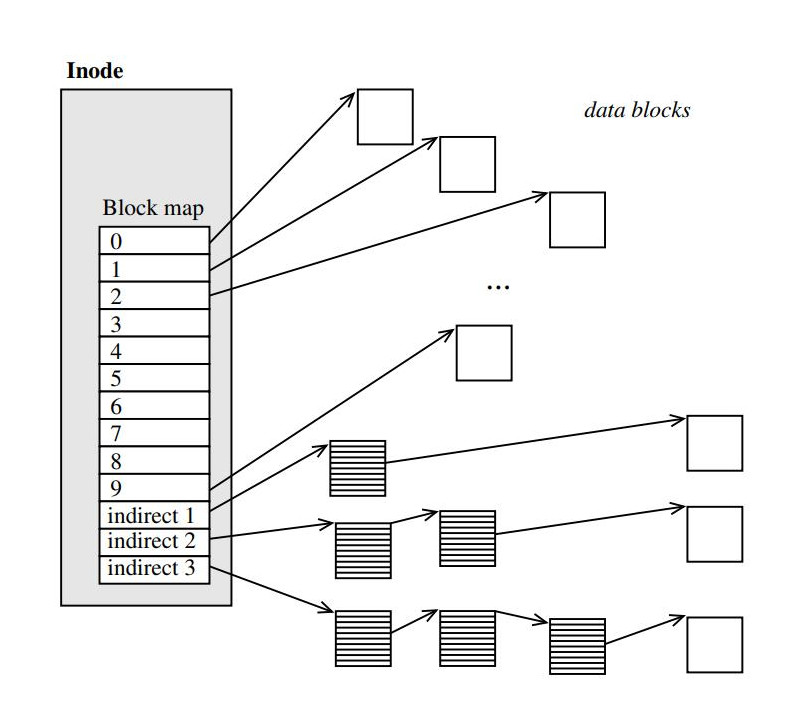
\includegraphics{6.2.2.jpg}}
    \caption{z prezentace IOS: Souborove systemy, slide 23 - odkazy v i-uzlech}
\end{figure}

\newpage

\subsubsection{Pocty odkazu}
\begin{itemize}
    \item neprimy odkaz 1. urovne - pri 4 KiB clusteru je to 1024 odkazu (1 odkaz = 4B) = 1024 datovych bloku,
    \item neprimy odkaz 2. urovne - pri 4 KiB clusteru je to $1024^2$ odkazu = stejny pocet datovych bloku,
    \item neprimy odkaz 3. urovne - pri 4 KiB clusteru je tam $1024^3$ odkazu = stejny pocet datovych bloku \\
\end{itemize}

\subsubsection{Limit maximalni velikosti souboru}

Poctem primych odkazu neprimeho odkazu 3. urovne je dan maximalni pocet bloku, ktere je mozne v tomto souborovem systemu ulozit. Teoreticky limit velikosti souboru je tak:
$$10 * D + N * D + N^2 * D + N^3 * D$$
kde $D$ je velikost bloku v bajtech (bezne 4096B), $M$ je velikost odkazu na blok v bajtech (bezne 4B), $N = D/M$, je pocet odkazu v bloku. \\

Toto omezeni velikosti je pouze jednim z omezenim, ktere velikosti souboru omezuji. \textbf{Dalsi omezeni jsou dana:}
\begin{itemize}
    \item dalsimi datovymi strukturami a typy, ktere pouziva FS (napr. datovy typ delky souboru v bajtech v i-uzlu),  
    \item strukturami VFS (veskera prace s jakymkoli filesystemem musi projit pres VFS),
    \item rozhranim jadra,
    \item architekturou systemu (32b - velikost souboru bude 32b cislo + MSB je pouzit pro indikaci chyby [-1 bit pro data] - soubory maximalne do 2 GiB nebo dnes bezna architektura 64b - 64b velikosti) \\
\end{itemize}

\textbf{Existuje Large File System Support}, kde ve 32b systemu se nahradi vsechny udaje kde se pracuje s velikosti vetsim datovym typem - podpora souboru \textit{vetsich jak 2 GiB}. \\

\textbf{linux:} \\[0.5em]
\textit{du [soubor]} vypise zabrane misto v blocich vc. rezie (metadat) \\[0.2em]
\textit{ls -l [soubor]} vypise velikost souboru v bajtech (pouze uzitecna data) \\[0.2em]
\textit{df} vypise volne misto na discich \\[0.2em]
\textit{ls -i [soubor]} zpristupni cislo i-uzlu souboru \\[0.2em]
\textit{is -e /dev/... n} - vypis i-uzlu n na /dev/... \\[0.2em]
\textit{dumpe2fs} - zakladni informace o souborovem systemu ext2,3,4 \\[0.2em]
\textit{/dev/zero} je soubor typu zarizeni generujici proud 0 \\[0.2em]
\textit{dd if=[source] of=[dest]} je nizkourovnove kopirovani \\

\newpage

\subsubsection{Vyhody a nevyhody architektury FS}
Neboli proc bylo navrzen FS prave tak, jak je. Architektura FS je totiz ovlivnena snahou o minimalizaci jejich rezie s relativne pomalymi disky (HDD, SDD), jedna se zejmena o bezne operace se soubory, jako je pruchod soubourem (otevru - prochazim od zacatku do konce) ci presun (seek), zvetsovani ci zmensovani (vc. mazani) souboru. \\

\textbf{Je nutne vzit do uvahy, z jakych (mikro)operaci se tyto operace sestavaji}. Jsou to operace:
\begin{itemize}
    \item vyhledavani adresy prvniho nebo urciteho bloku souboru,
    \item vyhledavani nasledujicich bloku,
    \item pridani ci odebrani bloku,
    \item alokace ci dealokace volneho souboru (informace o volnych oblastech, minimalizace externi fragmentace) \\
\end{itemize}

FS a jeho naslednici UFS, EXT2, EXT3 (EXT4 uz neni jeho naslednik!) predstavuji kompromis s ohledem prevazne na male soubory. (tyto fs funguji skvele pro male soubory - u vetsich souboru je nutne prochazet ci menit vetsi objem metadat) \\

Jistou optimalizaci pouzivanou i u klasickych filesystemu pro male soubory je ulozeni dat primo do i-uzlu. (pokud se tam data vlezou). \\

\textbf{definice:} \\[0.5em]
\textit{symbolicky odkaz} je soubor odkazujici na jiny soubor (pouziva ulozeni dat primo do i-uzlu) \\[0.2em]
\textit{rychle symlinky} maji data v i-uzlu \\[0.2em]
\textit{pomale symlinky} maji data mimo i-uzel

\newpage

\subsection{Jine zpusoby organizace souboru}
\subsubsection{Kontinualni ulozeni}
\begin{itemize}
    \item neboli spojite ulozeni souboru na disku,
    \item na disku je jeden spojity usek dat reprezentujici soubor,
    \item vyhodami jsou rychle vyhledani adresy 1./urciteho bloku nebo vyhledavani nasledujicich bloku,
    \item nevyhody: soubory nebude mozne jednoduse zvetsovat pokud budou prilis blizko u sebe (bude nutne jej presunout na jine volne a vetsi misto, pokud to pujde ci provest defragmentaci a pote zvetsit soubor)
    \item nepouziva se prilis (kvuli sve nevyhode) \\
\end{itemize}

\subsubsection{Zretezene seznamy alokacnich bloku}
\begin{itemize}
    \item kazdy alokacni blok obsahuje sva (uzitecna) data a na konci obsahuje odkaz na nasledujici alokacni blok,
    \item vyhodami jsou rychly pristup na zacatek ci pruchod daty,
    \item nevyhodou je presun na nahodne misto v souboru - nutnost precist cely soubor az po dany blok (1 GiB soubor, chci posledni blok - musim precist cely),
    \item dalsi nevyhodou je rozprostreni metadat po celem disku - pri drobne chybe na disku prijdu o data (tedy i metadata, kde jsou odkazy na nasledujici bloky) a dojde k velke ztrate dat (vsechna data "za" ztracenymi daty jsou nepristupna),
    \item neni prilis vhodna, nicmene se pouziva v souborovych systemech FAT \\
\end{itemize}

\subsubsection{FAT}
\begin{itemize}
    \item File Allocation Table,
    \item od zretezenych seznamu se lisi tim, ze seznamy popisujici rozlozeni souboru na disku jsou ulozeny v separatni oblasti na disku (tzv. FAT),
    \item kde jsou tato data koncentrovana - rychleji se prohledavaji, lze vytvorit tak vice kopii FAT (prevence okamzite ztraty dat pri chybe),
    \item stale vznikaji problemy s rychlosti pri nahodnem pristupu (stale jde o zretezeny seznam)
    \item tabulka je pole, ktere obsahuje pro kazdy blok na disku 1 polozku, kazda polozka obsahuje odkaz na dalsi blok/polozku,
    \item pouziva se i dodnes (a je to velmi rozsirene), protoze je to jednoduche (napr. vestavene systemy) \\
\end{itemize}

\newpage

\subsubsection{B+ stromy}
\begin{itemize}
    \item jsou datovou strukturou prevzatou z databazovych systemu,
    \item maji dva typy uzlu - vnitrni a listove,
    \item vnitrni uzly jsou koren, jeho naslednici krome listovych, obsahuji odkaz na naslednika a vyhledavaci klic,
    \item listove uzly take obsahuji odkazy a vyhledavaci klice, odkazy vedou na data na disku, posledni odkaz na poslednim listu odkazuje na list na stejne urovni (jsou tak propojeny linearnim seznamem),
    \item pouzivaji se za ucelem popisu rozlozeni dat na disku (obsah souboru, pote vyhledavaci klic bude offset - cislo logickeho bloku v ramci souboru) nebo se pouzivaji pro adresare (klice budou jmena souboru) nebo pro popis celeho obsahu disku (klic je dvojice i-uzel a posuv souboru) \\
\end{itemize}

\textbf{Vyhledavani v B+ stromu:}
\begin{itemize}
    \item pri hledani klice (k) se podivam, zda je klic mensi jak klic k0, pokud ano, pujdu nize, kde je k00, pokud ne, zjistim, jestli je klic mezi k0 a k1, pokud ano, jdu druhym smerem, opakuji po kn,
    \item pokud jsem niz, opakuji to same co vys az nedojdu k listovym uzlum,
    \item zde hledany klic najdu nebo zjistim ze v teto strukture klic neni
    \item pote mam odkaz na datovy blok,
    \item v pripade ze chci cist dal, tak jdu linearne po sobe po nasledujicich listovych uzlech \\
\end{itemize}

\begin{figure}[htb]
    \centering
    \scalebox{2}{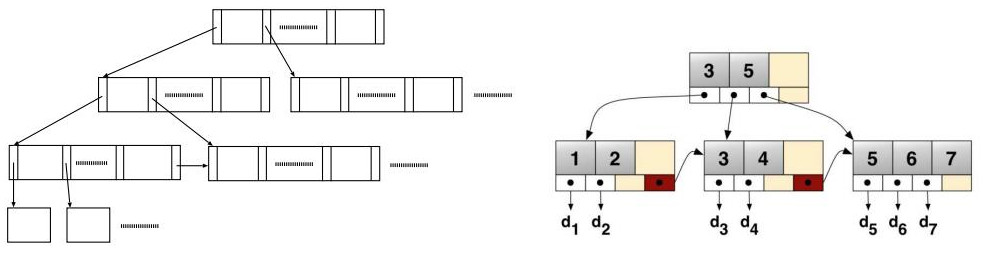
\includegraphics{6.3.4.jpg}}
    \caption{z prezentace IOS: Souborove systemy, slide 27 - B+ strom}
\end{figure}

\newpage

\textbf{Prace s B+ stromy:}
\begin{itemize}
    \item jsou zde limity jak moc/malo maji byt uzly zaplneny (strom se udrzuje vyvazeny) - pro uzly s $m$ odkazy mame klice $0, 1$, .. az $m - 2$ klicu (odkazu je o 1 mene nez klicu + cislovani od 0), 
    \item pokud je strom tvoren solo korenem - nejmene muze mit $1$ odkaz, maximalne $m - 1$ odkazu (posledni odkaz je pouzit jako ukoncovac seznamu listu),
    \item pokud to neni solo koren, tak ma nejake nasledniky, minimalne jich ma tak $2$, maximalne $m$,
    \item vnitrni uzel ma tak $\frac{m}{2}$ (zaokr. nahoru) az $m$ odkazu, list $\frac{m}{2} - 1$ (opet $\frac{m}{2}$ zaokr. nahoru) az $m - 1$ odkazu,
    \item vlozeni:
    \begin{itemize}
        \item nejprve projdeme stromem od korene k listum,
        \item najdeme kam chceme vlozit,
        \item podivame se, zda ma list volny odkaz,
        \item pokud ano - pouzijeme ho, pokud ne - list se rozstepi na 2 poloviny a podivam se o uroven vys, zda je mozne namisto 1 listu linkovat 2 listy,
        \item pokud ano - prida se odkaz, pokud ne - nadrazeny uzel se musi rozstepit a postupovat o uroven vys,
        \item ... stepi se strom az pripadne se rozstepi koren a strom bude mit 2 koreny
    \end{itemize}
    \item ruseni:
    \begin{itemize}
        \item se opet od listove urovne, tak, ze se zrusi odkaz v listu,
        \item zkontroluje se, zda je uzel zaplneny v ramci danych limitu,
        \item pokud ano - gut, pokud ne - podivam se na sousedni uzly a pokud se provest prerozdeleni tak, aby byly vsechny uzly naplneny v ramci limitu,
        \item pokud se to nepodari, tak dojde ke slouceni listu,
        \item posunu se o uroven vys, zrusim jeden odkaz, zkontroluji opet limity, zopakuji to same,
        \item ... az se muze stat, ze se zrusi i koren \\
    \end{itemize}
\end{itemize}

B+ stromy a jeho varianty jsou pouzivany pro popis diskoveho prostoru v filesystemech jako
XFS, JFS, ZFS, Btrfs, ReFS, ..
v omezene podobe tzv. stromu extentu v EXT4, podobna struktura je i v NTFS \\

\textbf{definice:} \\[0.5em]
\textit{solo koren} = jediny koren

\newpage

\subsubsection{Extent}
\begin{itemize}
    \item pouziva se ke zrychleni prace s velkymi soubory,
    \item umoznuji zmensit objem metadat (je mozne rict, ze nektere alokacni bloky jsou ulozeny pospolu = vytvari extent), potom budu popisovat rozlozeni souboru po extentech (ne po alokacnich blocich),
    \item prinese lepe vyvazene indexove struktury,
    \item rychlejsi mazani,
    \item jsou pouzity snad ve vsech systemech s B+ stromy,
    \item B+ strom se snadno kombinuje s extenty (neplati pro klacicky Unixovy strom - protoze ve stromu jsou explicitne ulozene vyhledavaci klice, ale Unixovy nema v zadnych strukturach [i-uzel] ulozenou velikost datovych bloku [protoze jsou vsechny stejne a konstantni]) \\
\end{itemize}

Pokud pouzivame B+ stromy, tak rychlemu spojitemu pruchodu pomaha listova uroven, pokud je prolinkovani listu pouzito. Pro male soubory muze predstavovat B+ strom zbytecnou rezii (data se bud ulozi primo v i-uzlu nebo nebo z nej mame prime odkazy na extenty z i-uzlu [do max. 4 extentu]) \\

\textbf{definice:} \\[0.5em]
\textit{extent} je jednotka vystavena na bloky, posloupnost promenneho poctu alokacnich bloku (jdoucich za sebou logicky v souboru i fyzicky na disku) \\

\newpage

\subsection{EXT4}
Pouziva pro popis rozlozeni dat na disku strom extentu. Pro "male soubory" (mysleno soubory, na ktere je mozne se odkazovat az 4 extenty, pak tyto extenty budou odkazovane primo z i-uzlu; tldr soubory s malym poctem extentu) \\

\textbf{definice:} \\[0.5em]
\textit{strom extentu} je v principu B+ strom degradovany na maximalne 5 urovni, bez pouzivani vyvazovani (napr. prerozdelovani uzlu pri mazani) a zretezeni listu \\

\subsection{NTFS}
Zakladni datovou strukturou popisujici disk je MFT - Master File Table (ma pro kazdy soubor alespon 1 radek, na 0. radku popisuje samo sebe, 1. radek pripadne kopie MFT, pripadne metadata, pote obsahy souboru).  \\

\textbf{Obsah souboru muze byt reprezentovan bud:}
\begin{itemize}
    \item pokud jde o kratky soubor, bude ulozen v MFT v jeho radku (vcetne metadat),
    \item soubor je rozdelen na extenty (ty jsou odkazovane primo z radku souboru v MFT, tak ze v radce souboru jsou informace o pocatecnim VCN a LCN a pocet clustero, ktery dany extent obsahuje) - vyhledava se v tom stejne jako v B+ stromu
    \item pokud je extentu potreba vice nez se vleze na jeden radek, alokuji se pomocne radky (z hlavniho radku vedou odkazy na pomocne, z pomocnych vedou odkazy na disk) - prochazeni je opet ve stylu B+ stromu \\
\end{itemize}

\textbf{definice:} \\[0.5em]
\textit{VCN} - virtual cluster number, logicky blok souboru \\[0.2em]
\textit{LCN} - logical cluster number, cislo fyzickeho bloku (souvisi s tim ze je to na logickem disku) \\

\subsection{Organizace volneho prostoru na disku}
V klasickem Unixovem FS a rade jeho nasledovniku (UFS, EXT2, 3), take v NTFS se pouzivaji bitove mapy, kde pro kazdy blok mam 1 bit. V bitove je mozne pote vyhledavat pomoci bitovych mask - zrychli vyhledavani. \\

\textbf{Dalsi mozne zpusoby organizace volneho prostoru:}
\begin{itemize}
    \item pouziji se alokacni seznamy (zretezeni volnych bloku na disku),
    \item zretezeni volnych polozek v tabulce (FAT),
    \item B+ strom (udrzovani informaci o tom, kde je volne misto, adresace velikosti a/nebo offsetem)
    \item volny prostor muze byt take organizovan po extentech. \\
\end{itemize}

\newpage

\subsection{Deduplikace}
\begin{itemize}
    \item podporovana ZFS, NTFS, Btrfs, XFS, (ext4 ne) ..
    \item snazi se odhalit opakovane ukladani stejnych dat na disk a ulozi je pouze jednou a odkazuje se na ne vicenasobne.
    \item systemy s deduplikaci se snazi takova data detekovan (sekvence bitu, bloku, extentu, ..)
    \item zalozeno na kryptografickem hashovani (hledaji se data se stejnym popisem, urci se shoda),
    \item muze byt realizovano pri zapisu nebo dodatecne (zadost uzivatele),
    \item muze usporit diskovy prostor (pri virtualizaci, na mail serverech, repozitare, ..), pametovy prostor i cas (zamezi se opakovanemu cteni i zapisu),
    \item pri mensim objemu duplikace muze naopak zvysit spotrebu CPU casu, spotrebu pametoveho i diskoveho prostoru \\
\end{itemize}

\textbf{Rozdil oproti copy-on-write:}
\begin{itemize}
    \item copy-on-write se muze uchytit (klony, snimky) pouze tehdy, pokud duplikaty vzniknou cinnosti samotneho filesystemu (napr. vytvoreni virtualek),
    \item zatimco deduplikace aktivne vyhledava duplikaty (napr. uzivatel, co stahuje stejne reklamni letaky) \\
\end{itemize}

\subsection{Typy souboru v UNIXu}
\begin{itemize}
    \item - je obycejny soubor,
    \item d adresar,
    \item b blokovy specialni soubor,
    \item c znakovy specialni soubor,
    \item l symbolicky odkaz (symlink),
    \item p pojmenovana roura,
    \item s socket \\
\end{itemize}

\textbf{definice:} \\[0.5em]
\textit{specialni soubor} je typ souboru reprezentujici hardwarove zarizeni (disk, hw, pamet) se kterym se komunikuje po blocich nebo znacich \\[0.2em]
\textit{symbolicky odkaz} je soubor obsahujici jmeno jineho souboru (odkazuje na nej) \\

\newpage

\subsection{Adresar}
Je to kolekce jinych souboru na nejvyssi urovni abstrakce. Soubor obsahuje mnozinu dvojic jmeno a unikatni ciselne oznaceni. \\

\textbf{Jmeno souboru:}
\begin{itemize}
    \item drive limit 14 znaku, dnes az 255 (na konci musi byt '\verb|\0|')
    \item ve jmene nesmi byt / nebo '\verb|\0|' \\
    \item lati ze kazdy adresar v POSIX systemu vzdy obsahuje minimalne 2 jmena: . (odkaz na sebe) a .. (odkaz na rodicovsky adresar)
\end{itemize}

\textbf{Cislo souboru:}
\begin{itemize}
    \item u klasickeho souboru unixu je to cislo i-uzlu,
    \item v jinych pripadech to slouzi jako klic do dane vyhledavaci struktury (B+ strom) \\
\end{itemize}

\textbf{Implementace adresaru:}
\begin{itemize}
    \item pouzivaji se ruzne pristupy, lisi se jednoduchosti implementace ci rychlosti vyhledavani (vkladani),
    \item seznam (obsah souboru bude tvorena seznamem),
    \item B+ stromy (v NTFS, XFS, JFS, APFS nebo EXT3/4 - ty pouzivaji H-stromy: 1-2 urovne, bez vyvazovani a vyhledava se na zaklade zahashovaneho jmena)
    \item hashovaci tabulky v napr. ZFS \\
\end{itemize}

Soubor v UNIXu muze mit vice jmen. Dalsi jmena se vytvari pomoci prikazu ln \\

\textbf{linux:} \\[0.5em]
\textit{ln [existujici jmeno] [nove jmeno]} vytvori dalsi jmeno souboru \\

\newpage

\subsection{Montovani disku}
\textbf{Princip motnovani disku:}
\begin{itemize}
    \item v UNIXu neni zadne oznaceni disku (A:, C:, ..), ale mame jeden adresarovy "strom",
    \item v systemu je jeden korenovy logicky disk,
    \item dalsi logicke disky se pripojuji programem \textit{mount} do existujiciho adresaroveho stromu (korenovy adresar zarizeni se "slepi" s adresarem v mem stromu) \\
\end{itemize}

Pripojovaci volby se mohou zadavat rucne (v terminalu) nebo se mohou predpripravit do /etc/fstab. Soubor /etc/mtab obsahuje tabulku aktualne pripojenych disku. \\

\textbf{Novejsi technologie umoznuji automaticke montovani nove pripojenych zarizeni:}
\begin{itemize}
    \item na linuxu bezne pracuje system udev, ktery
    \item rozpozna, ze se pripojilo nove zarizeni,
    \item vytvori odpovidajici soubor typu blokove zarizeni (/dev/..),
    \item informuje o tom zbytek systemu pomoci sbernice D-Bus,
    \item aplikace typu spravce souboru pak muze provest automaticke montovani (a dalsi akce),
    \item prednost ma vzdy /etc/fstab,
    \item identifikace se nemusi provadet jen zarizenim (/dev/..), je mozne si vygenerovat unikatni identifikator a pouzivat ten (UUID) \\
\end{itemize}

\textbf{Technologie Automounter:}
\begin{itemize}
    \item subsystem jadra,
    \item pripojuje automaticky potrebne disky v situaci, kdy se pokusime pristoupit na pozici adresaroveho stromu, kam by takovyto disk mel byt pripojeny (napr. na /mnt ma byt pripojena flashka, nemusi byt mountla, uzivatel da cd /mnt, automounter to zjisti a pripoji flashku sem),
    \item ma take nejaky cas, po kterem disk automaticky odpoji, pokud se nim nepracuje  \\
\end{itemize}

\textbf{Union mount:}
\begin{itemize}
    \item technologie umoznujici sjednocujici montovani (v unixu dostupna pomoci filesystemu UnionFS),
    \item umoznuje do jednoho pripojneho bodu namontovat vice disku,
    \item obsah pripojneho bodu je sjednocenim obsahu disku,
    \item v pripade, ze na vice discich jsou soubory se stejnymi jmeny vznikaji kolize, ty se resi napr. preddefinovanim priorit pripojovanych filesystemu a zpristupni se soubor daneho jmena z logickeho disku, ktery ma nejvetsi prioritu
    \item UnionFS ma copy-on-write semantiku, coz umoznuje emulaci prepisovani neprepisovatelnych medii (v 1 vetvi CD, neprepisovatelne, na tom je linuxova distribuce, soucasne se do stejneho bodu pripoji bezny disk s vyssi prioritou - na zacatku bude disk prazdny, budou videt vsechny soubory z CD, jakmile se pokusim prepsat neco, UnionFS vytvori kopii na prepisovatelny disk) \\
\end{itemize}

\textbf{linux:} \\[0.5em]
\textit{mount [co-pripojit] [kam-pripojit]} pripoji logicky disk \\

\newpage

\section{}
\textbf{Sedma prednaska:} Pokracovani Spravy souboru. Symbolicke odkazy, 
\subsection{Symbolicke odkazy}
\begin{itemize}
    \item je samostatny soubor odkazujici na existujici soubor,
    \item system pri otevreni automaticky otevre cilovy souboru - vicenasobne zpracovani cesty (ceska k symlinku a cesta uvnitr nej),
    \item soubor se smaze, pokud jeho pocet jmen klesne na 0,
    \item symlink muze odkazovat na neexistujici soubor (pri otevreni dojde k chybe),
    \item muze odkazovat i na jiny logicky disk,
    \item lze ze symlinku vytvorit cyklkus (jeden odkazuje na druhy a druhy na prvni) - v systemy je preddefinovany maximalni pocet na sebe odkazujicich symlinku (pri prekroceni dojde k chybe),
    \item symlinky lze vyuzit napr. pri upgradu systemu. \\
\end{itemize}

\textbf{Rozdil rychlych/pomalych symlinku:}
\begin{itemize}
    \item obsahem symlinku je jmeno ciloveho souboru,
    \item pokud jmeno souboru neni prilis dlouhe (vleze se do i-uzlu), potom se ulozi do i-uzlu = rychly symlink (staci otevrit jen i-uzel),
    \item pokud se jmeno nezleve do (i-uzlu), alokuji se normalne alokacni bloky na disku = pomaly symlink \\
\end{itemize}

\textbf{linux:} \\[0.5em]
\textit{ln -s [existujici soubor] [symbolicky odkaz]} vytvori symbolicky odkaz \\

\newpage

\subsection{Blokove a znakove specialni soubory} \label{blok-char-hw}
Soubory reprezentujici rozhrani souboroveho systemu k fyzickym (opravdovy hw) ci virtualnim zarizenim (xterminaly, ..). Souborovy system vyvtari souborove rozhrani, tim umoznuje tyto soubory pri urcitych operacich identifikovat (jmeno soubory, napr. /dev/sdX), s celym zarizenim lze take pracovat jako se souborem. \\

Typicky zarizeni sidli v adresari /dev \\

\textbf{Bezne typy zarizeni:}
\begin{itemize}
    \item /dev/hda - (drive)oznaceni pro prvni fyzicky disk na prvnim ATA/PATA rozhrani
    \item /dev/hda1 - (drive) prvni logicky disk na hda
    \item /dev/sda - prvni fyzicky disk SCSI, navic i disky SATA/PATA (jadro nad temito disky emuluje SCSI)
    \item /dev/mem - obsah pameti (RAM)
    \item /dev/zero - nekonecny zdroj 0 bajtu
    \item /dev/null - soubor typu cerna dira - cokoli se do nej zapise, do se zahodi (presmerovani vystupu programu tak, aby nas neotravoval), pri cteni se tvari jako prazdny soubor
    \item /dev/random - generator nahodnych cisel
    \item /dev/tty - terminal
    \item /dev/lp0 - tiskarny
    \item /dev/mouse - mys
    \item /dev/dsp - zvukova karta
    \item /dev/loop - zarizeni typu (smycka) loop mi umoznuje pripojit soubor jako disk (obraz souboroveho systemu) k adresari, jakoby se jednalo o novy fyzicky disk \\
\end{itemize}

Tato oznaceni zavisi na pouzitem systemu (Linux, distribuce, ..). Vyhoda zavedeni specialnich souboru je, ze umoznuji identifikovat zarizeni, se kterymi chci pracovat. \\

\newpage

\subsection{Pristupova prava}
V UNIXu jsou typicky rozlisena na prava pro vlastnika, skupinu vlastniku a ostatni.
Existuje rozsireni ACL (access control list). \\

\textbf{Uzivatele:}
\begin{itemize}
    \item jsou definovani administratorem systemu (root) v /etc/passwd,
    \item maji definovana sva UID - uzivatelska cisla (root UID = 0),
    \item kazdy soubor ma sveho vlastnika,
    \item chown - zmena vlastnika souboru (pouze root), \\
\end{itemize}

\textbf{Skupiny:}
\begin{itemize}
    \item definuje administrator systeu v /etc/group,
    \item maji sva GID - cislo identifikujici skupinu uzivatelu,
    \item v kazde skupine je uvedeno, kdo do te skupiny patri,
    \item kazdy uzivatel muze byt clenem vice skupin,
    \item jedna z nich je aktualni (pouziva se pri vytvareni souboru) \\
\end{itemize}

\textbf{linux:} \\[0.5em]
\textit{groups} - vypis skupin uzivatele \\[0.2em]
\textit{chgrp} - zmena skupiny souboru \\[0.2em]
\textit{newgrp} - novy shell s jinym aktualnim GID \\

\newpage

\subsection{Typy pristupovych prav}
\textbf{Obycejne soubory:}
r, w, x - pravo cist, zapisovat a spustit soubor jako program. \\

\textbf{Adresare:}
\begin{itemize}
    \item r - pravo cist obsah adresare,
    \item w - pravo zapisovat (vytvaret a rusit soubory),
    \item x - pravo pristupovat k souborum v adresari (moznost cd adresar, ls -l adresar, ..) \\
\end{itemize}

\textbf{Typicky vystup pristupovych prav je:}
\begin{itemize}
    \item ve formatu: [1:typ souboru] [3:prava vlastnika] [3:prava skupiny] [3:prava ostatnich]
    \item napr.: -rwx---r-- (ciselne vyjadreni v 8 soustave 0704)
    \item je obycejny soubor, vlastnik ma vsechna prava, skupina zadna a ostatni maji prava na cteni \\
\end{itemize}

Zmena pristupovych prava se deje pomoci chmod. (Pro nespustitelne soubory je bezny chmod 0644). \\

\textbf{linux:}
\textit{chmod [1:pro koho][nova prava] [soubor/y]} zmena pristupovych prav \\

\subsection{Sticky bit}
Priznak, ktery pokud bude prirazen nejakemu adresari, tak se vytvori adresar, ve kterem i pres pravo cteni a zapisu souboru mohou uzivatele rusit pouze ty soubory, ktere sami vytvorili. (typicky adresar /tmp) (tldr: uzivatel muze mazat, ale pouze to co vlastni) \\

\subsection{SUID, SGID}
\textbf{S procesy jsou spojeny identifikatory jako jsou:}
\begin{itemize}
    \item UID - realna identifikace uzivatele (cislo uzivatele, ktery dany proces spustil)
    \item EUID - efektivni identifikator pouzivany pro kontrolu pristupovych prav (vetsinou stejne jako UID)
    \item GID - realna identifikace skupiny (kdo spustil proces)
    \item EGID - efektivni GID, (stejne chovani jako u EUID) \\
\end{itemize}

Vlastnik programu muze propujcit sva prava komukoliv, kdo spusti program s nastavenym SUID. (tldr: propujci se prava mezi uzivateli, bezne se to pouziva v pripadech, kdy administrator propujcuje sva prava uzivatelum, napr. passwd) \\

Pri pouziti SUID bude UID = uzivatele, ktery proces spustil a EUID = identifikace vlastnika (= ktery prava pujcil). Pokud budou prava propujcena (pouzito SUID), misto x se vypise s, pokud tam x neni, vypise se S. \\

\subsection{Typicka struktura adresaru v UNIXu}
\textbf{FHS - Filesystem Hierarchy Standard (Linux), (cast hierarchie):}
\begin{itemize}
    \item /bin - programy pro vsechny uzivatele (spustitelne, mohou byt zapotrebi pri bootovani - musi byt dostupne lokalne)
    \item /boot - soubory pro zavadec systemu (obrazy jadra, pocatecni fs)
    \item /dev - specialni soubory - rozhrani zarizeni
    \item /etc - konfiguracni soubory pro system i aplikace
    \item /home - domovske adresare uzivatelu
    \item /lib - sdielne knihovny a moduly jadra
    \item /media - pripojny bod pro prenosna zarizeni
    \item /mnt - pripojny bod pro docasne filesystemy
    \item /proc - informace o procesech a jadru
    \item /root - domovsky adresar superuzivatele
    \item /run - docasne informace o bezicim systemu (demony)
    \item /sbin - programy pro superuzivatele (nutne pro bootovani, ne vse je spustitelne superuzivatelem)
    \item /sys - informace o jadru, zarizenich, modulech, ..
    \item /tmp - docasne pracovni soubory (obsah se maze pri restartu)
    \item /usr - obsahuje dale adresare a
    \begin{itemize}
        \item soubory, ktere nejsou nutne pri zavadeni systemu, struktura je zde podobna jako u / :
        \item bin, sbin, lib,
        \item include (hlavickove soubory),
        \item share (soubory je mozne sdilet nezavisle na architekture),
        \item local (koren dalsi hierarchie urcena pro lokalni nestandardni instalace programu),
        \item src (zdrojove texty jadra)
    \end{itemize}
    \item /var - soubory menici se za behu systemu
    \begin{itemize}
        \item obsahuje log (zaznamy o cinnosti systemu), 
        \item spool (pomocne soubory pro tisk),
        \item mail (postovni prihradky uzivatelu) \\
    \end{itemize}
\end{itemize}

\newpage

\textbf{Nove tema: Datove struktury a algoritmy pro vstup/vystup}
\subsection{Pouziti vyrovnavacich pameti}
Cilem pouziti cache (vyrovnavacich pameti) je minimimalizace poctu pomalych operaci s periferiemi (disky). Hierarchie:
kolekce, sbirka dilcich vyrovnavacich pameti (s velikosti 1 alokacniho bloku, ci nasobku), nazyva se buffer-pool, muze mit pevnou velikost, spise je promenna. \\

\newpage

\subsection{Operace se soubory}

\subsubsection{Cteni}
\textbf{Prvni cteni alokacniho bloku:}
\begin{itemize}
    \item zjisti se, zda je blok v pameti,
    \item pokud ne, naalokuje se novy blok, muze se vyuzit jiz nejaky systemem predalokovany a nevyuzity,
    \item nactou se data z disku, presunou se do vyrovnavaci pameti,
    \item vyrovnavaci pamet je v prostoru jadra (bezne procesy zde nemaji pristup),
    \item vykousne se z nactenych dat tu cast, o kterou ma uzivatel/proces zajem,
    \item nakopiruje se to do adresoveho prostoru uzivatelskeho prostoru \\
\end{itemize}

\textbf{Pri dalsim cteni:}
\begin{itemize}
    \item nejprve se opet vyhleda, zda je blok v pameti,
    \item pokud ano,
    \item nebude se cist z disku, pouze se z alokacniho bloku vykousne cast, o kterou ma uzivatel/proces zajem,
    \item tato cast se uzivateli preda \\
\end{itemize}

\subsubsection{Zapis}

\textbf{Postup pri zapisu:}
\begin{itemize}
    \item nejprve se zjisti, zda je blok v pameti,
    \item pokud ne, prideli se vyrovnavaci pamet,
    \item nactou se data z disku do vyrovavaci pameti,
    \item jadro prevezme od procesu, ktery chce zapisovat data, ktera chce zapsat,
    \item prepise jimi danou cast alokacniho bloku, dirty bit se zmeni (0 na 1),
    \item operace konci (neprovede se zapis na disk),
    \item casem se provede zpozdeny zapis na disk a vynuluje se dirty bit \\
\end{itemize}

System sam od sebe s periodou prepisuje cache na disky, lze si to vynutit pomoci sync ci fsync. \\

Pokud je znamo, ze se prepise cely alokacni blok (nebo se jedna o novy blok), buffer se vynuluje a nenacitaji se data z disku do cache. \\


\textbf{definice:} \\[0.5em]
\textit{dirty bit} je indikator toho, jestli jsou data cache sladena s obsahem na disku (0 - data v cache = disk, 1 - data cache != data disk - nuluje se zpozdenym zapisem) \\

\subsubsection{Otevreni souboru pro cteni}
Pokud soubor jeste \textbf{nebyl otevren}:
\begin{itemize}
    \item system musi vyhodnotit cestu a naleznou cislo i-uzlu (resp. cislo datove struktury poskytujici informace o danem souboru - pristupova prava, kde jsou ulozena data),
    \begin{itemize}
        \item pri tom se postupne nacitaji i-uzly vsech adresaru vedouci na soubor,
        \item pote se nacte i-uzel souboru,
        \item system pouziva d-entry cache (specialni vyrovnavaci pamet pouzita pro preklad odpovidajicich jmen souboru na i-uzel) 
        \item dale alokuje polozku v tabulce V-uzlu,
    \end{itemize}
    \begin{itemize}
        \item z disku se nacte i-uzel,
        \item vlozi se do nove alokovane polozky = vznika rozsirena pametova kopie i-uzlu,
        \item budou tam i informace navic (jako je pocet odkazu na danou polozku - danym i-uzlem muze pracovat vice procesu).
    \end{itemize}
    \item v tabulce popisovacu vytvorime novou polozku,
    \begin{itemize}
        \item tato tabulka je ulozena v zaznamu o procesu (tabulka procesu v jadre) nebo v uzivatelske oblasti,
        \item pouzije se nejnizsi volna polozka zde,
        \item naplni se odkazem na polozku v tabulce otevrenych souboru,
    \end{itemize}
    \item pokud se otevreni vydari, vrati se cislo popisovace, pokud ne, tak vraci -1. \\
\end{itemize}

Tolik tabulek se pouziva pro zamezeni duplikaci udaju. Behem otevirani se provadi kontrola pristupovych prav. Soubor je mozne otevrit v rezimu pro cteni, zapis, cteni i zapis. \\

Dalsi otevreni souboru (\textbf{jiz jednou otevreny}):
\begin{itemize}
    \item opet se vyhodnoti cesta k souboru a ziska se cislo i-uzlu,
    \item system se podiva do tabulku V-uzlu,
    \item zjisti, ze i-uzel uz tam je,
    \item nebude se znovu i-uzel nacitat z disku, pouze se zvysi citac pouziti i-uzlu,
    \item tabulka V-uzlu musi byt vyhledavaci (typicky vyhledaci struktury jako hash tabulka, strom, ..),
    \item naalokuje se nova polozka v tabulce otevreni (naplni se rezimem otevreni, pozici, odkazem na sdileny V-uzel),
    \item naalokuje se nove poloza ve file descriptoru ukazujici na nove otevreni (a ta se vrati) \\
\end{itemize}

\newpage

\textbf{Je mozne pridavat i dalsi identifikatory, napr.:}
\begin{itemize}
    \item priznak, ze ma byt soubor vytvoren pokud neexistuje,
    \item pokud existuje, ma byt zkracen na 0,
    \item otevrit v rezimu pridavani (kdekoli je aktualne ukazovatko v souboru, tak v pripade zapisu se automaticky posune na konec a tam se prida),
    \item synchronni zapis (operace zapisu skonci az tehdy, kdyz se data zapisou opravdu na disk) \\
\end{itemize}

\textbf{Pri chybe:}
\begin{itemize}
    \item open vraci -1,
    \item nastavi se chybovy kod, ktery blize popisuje co se stalo (do knihovni promenne errno),
    \item existuji standardni chybove kody,
    \item lze pouzit standardni knihovni funkci perror \\
\end{itemize}

\textbf{linux:} \\[0.5em]
\textit{fd = open([jmeno souboru], [rezim]);} otevre soubor \\[0.2em]
\textit{V-uzly} je tabulka i-uzlu filesystemu VFS \\[0.2em]
\textit{tabulka popisovacu} je pole s radky cislovanymi od 0 (0 - stdin, 1 - stdout, 2 - stderr) \\[0.2em]
\textit{tabulka procesu} v jadre je cast adresoveho prostoru, ve kterem ma jadro ulozene pomocne informace k procesum a ma sem pristup pouze jadro \\[0.2em]

\subsubsection{Cteni a zapis z/do souboru}
\textbf{Cteni:}
\begin{itemize}
    \item zkontroluje se platnost popisovace (otevreni popisovace, soubor pro cteni),
    \item pokud se jedna o prvni pristup, naalokuje se cache, nactou se data do cache a z cache se prislusna data pouziji,
    \item pokud uz jsou data v cache, nactou se odtud,
    \item predani se deje pozadovanych z cache (RAM, jadro) do pole (RAM, cache adresoroveho prostoru procesu),
    \item funkce vraci pocet opravdu prectenych bajtu nebo -1 pri chybe (+ nastavi errno). \\
\end{itemize}

\textbf{Zapis:}
\begin{itemize}
    \item funguje podobne jako read,
    \item pred vlastnim zapisem kontroluje dostupnost diskoveho prostoru a tento prostor alokuje (rezervuje),
    \item vraci pocet opravdu zapsanych bajtu nebo -1 \\
\end{itemize}

\newpage

\textbf{linux:} \\[0.5em]
\textit{read([popisovac], [adresa pameti, kam se ma zapsat], [kolik bajtu se ma nacist])} precte soubor \\[0.2em]
\textit{write ([popisovac], [adresa pameti, ze ktere se nactou data], [kolik bajtu se zapise])} zapis do souboru \\

\subsubsection{Primy pristup k souboru}
Nahodne presouvani v souboru. \textbf{Postup:}
\begin{itemize}
    \item zkontroluje zda je popisovac platny (je soubor otevren?)
    \item nastavi pozici offset bajtu od whence
    \begin{itemize}
        \item SEEK\_SET - napr. 200 - posunu se od 200 bajtu od zacatku,
        \item SEEK\_CUR - od aktualni pozice,
        \item SEEK\_END - od konce souboru),
    \end{itemize}
    \item nelze se posunou pred zacatek souboru,
    \item je ale mozne se posunout za konec souboru (a zapsat),
    \item vraci se vysledna pozice od zacatku souboru nebo -1 \\
\end{itemize}

Posunem za konec souboru a naslednym zapisem vznikaji tzv. ridke soubory (sparse files):
\begin{itemize}
    \item umoznuje na disku o nejake kapacite vytvorit soubor, ktery ma zdanlive vetsi velikost nez samotny disk,
    \item bloky do kterych se nezapisovalo nejsou alokovany a nezabiraji diskovy prostor (pri cteni se povazuji za 0),
    \item take muze vzniknout mazanim uprostred souboru (hole punching) \\
\end{itemize}

\begin{figure} [h]
    \centering
    \scalebox{2}{
\includegraphics{7.9.5.jpg}} \\
    \caption{z prezentace IOS: Sprava souboru - ridke soubory} 
\end{figure}

\textbf{linux:} \\[0.5em]
\textit{lseek([popisovac souboru], [offset], [oproti cemu se chci posouvat])} primy pristup k souboru \\

\newpage

\subsubsection{Zavreni souboru}
\begin{itemize}
    \item zkontroluje se platnost file descriptoru (je vubec otevreny?),
    \item uvolni se dana polozka v tabulce popisovacu,
    \item system se podiva na odkazovanou polozku v tabulce otevrenych souboru,
    \item snizi se pocitadlo o 1,
    \item pokud bude pocitalo != 0, uzavirani skonci,
    \item pokud bude pocitadlo == 0, pokracuje se do 
    \item prislusne polozky tabulky V-uzlu, snizi se zde pocitadlo o 1,
    \item pokud bude zde pocitadlo != 0, uzavreni skonci,
    \item pokud bude zde == 0, soubor se definitivne uzarve,
    \item uvolni se z pameti i-uzel z tabulky V-uzlu (se zmenenymi udaji - cas zapisu, pristupu, modifikace i-uzlu, ..),
    \item naplanuje se blok, ve kterem je i-uzel ulozen,
    \item casem se i-uzel zapise na disk,
    \item funkce vraci 0 nebo -1 pri chybe \\
\end{itemize}

Pokud se proces skonci, automaticky se zavrou vsechny jeho deskriptory. Uzavreni souboru nezpusobi ulozeni obsahu jeho vyrovnavaci pameti na disk. \\

\textbf{linux:} \\[0.5em]
\textit{close([popisovac souboru])} zavre soubor \\

\subsubsection{Duplikace deskriptoru souboru}
\begin{itemize}
    \item zkontroluje se platnost deskriptoru (je soubor otevren?),
    \item zkopiruje obsah puvodniho popisovace do noveho (odkaz ve fd tabulce se zkopiruje do dalsi polozky v teto tabulce - oboje ukazuji na stejnou polozku tabulky otevrenych souboru + inkrementuje se pocitadlo), 
    \item automaticky se novy deskriptor uzavre (pokud je otevren),
    \item vraci index nove vytvorene polozky nebo -1,
    \item typicke pouziti je u presmerovani (stdin/stdout) \\
\end{itemize}

\textbf{linux:} \\[0.5em]
\textit{dup([popisovac])} duplikace deskriptoru (duplikuje existujici popisovac do nejvyssiho volneho noveho) \\[0.2em]
\textit{dup2([popisovac], [novy popisovac])} duplikace deskriptoru (do ktereho popisovace se duplikuje) \\

\subsubsection{Ruseni souboru}
\begin{itemize}
    \item vyhodnoti se cesta, zkontroluje se platnost jmena souboru, pristupova prava (zapis),
    \item odstrani se pevny odkaz (=hard link) mezi jmenem souboru a i-uzlem,
    \item zmensi se pocet jmen v i-uzlu,
    \item pokud je pocet jmen == 0 a i-uzel nikdo nepouziva - i-uzel muze byt uvolnen a mohou byt uvolneny vsechny bloky souboru,
    \item dokud ma soubor alespon 1 jmeno nebo nema zadne jmeno ale je otevren alespon 1x, nelze soubor z disku opravdu smazat,
    \item funkce vraci 0 nebo -1 pri chybe \\
\end{itemize}

Je mozne provest unlink na otevreny soubor (smaze se az po jeho uzavreni) a pracovat s nim dale,
vyuziti pri instalacich novych verzich programu, ktere aktualne bezi. (upgradovat upgradovaci program) \\

\textbf{linux:} \\[0.5em]
\textit{unlink([jmeno soubor, prip. cesta])} rusi soubor \\[0.2em]
\textit{shred} - bezpecne mazani \\

\subsubsection{Dalsi operace se soubory}

\textbf{linux:} \\[0.5em]
\textit{creat, open} - vytvoreni souboru \\[0.2em]
\textit{rename} - prejmenovani souboru \\[0.2em]
\textit{truncate, ftruncate} - zkraceni souboru \\[0.2em]
\textit{fcntl, lock} - zamykani zaznamu \\[0.2em]
\textit{chmod, chown} - zmena atributu \\[0.2em]
\textit{utime} - umoznuje zmenit casy prace se soubory (neumoznuje zmenit cas modifikace i-uzlu) \\[0.2em]
\textit{stat} - ziskani atributu (velikost, prava, ..) \\[0.2em]
\textit{sync, fsync} - vynuceni si zapisu vyrovnavacich pameti \\

\subsubsection{Adresarove soubory}
Obsahuje dvojice cislo i-uzlu a jmena souboru. Adresare nelze zapisovat ci cist po bajtech.

\textbf{linux:} \\[0.5em]
\textit{mkdir} - tvori se adresare (vytvori polozky . a ..) \\[0.2em]
\textit{opendir} - otevre adresar \\[0.2em]
\textit{readdir} - cte adresar \\[0.2em]
\textit{closedir} - zavre adresar \\[0.2em]
\textit{creat, link, unlink} - modifikace se provadi neprimo vytvarenim/modifikacemi souboru \\

\subsubsection{Blokove a znakove specialni soubory}
Predstavuji rozhrani k blokovym / znakovym zarizenim (/dev/..., viz. \ref{blok-char-hw})
\begin{itemize}
    \item lze je vytvorit pomoci mknod,
    \item typicky tyto soubory vytvari jadro ci demoni (udev, devd - pri pripojeni zarizeni se vytvori automaticky prislusny soubor) \\
\end{itemize}

Pri pouziti beznych souborovych operaci jadro mapuje operace na odpovidajici podprogramy, ktere ty operace implementuji pro dany typ zarizeni s vyuzitim \textbf{tabulek}:
\begin{itemize}
    \item znakovych zarizeni,
    \item blokovych zarizeni \\
\end{itemize}

Tyto tabulky obsahuji ukazatele na funkce implementujici prislusne operace v ovladacich danych zarizeni. \\

Specialni soubory na disku zabiraji \textbf{pouze i-uzel, krome beznych udaji maji v i-uzlu typ souboru a 2 udaje}:
\begin{itemize}
    \item hlavni cislo,
    \begin{itemize}
        \item major number,
        \item udava typ zarizeni
        \item odkazuje do tabulky zarizeni (hlavni cislo = n-ty radek tabulky),
    \end{itemize}
    \item vedlejsi cislo 
    \begin{itemize}
        \item minor number, 
        \item udava instanci zarizeni
        \item pouziva se jako parametr pri volani urcite operace - parametr funkce ovladace (cislo = ktere zarizeni se ma presne pouzit)
    \end{itemize}
    \item typ souboru urcuje tabulku (blok, znak.) \\
\end{itemize}

\textbf{linux:} \\[0.5em]
\textit{mknod} vytvori specialni soubory \\[0.2em]
\textit{ovladac} je sada podprogramu pro rizeni urciteho typu zarizeni (nebo viz xx nebo viz xx) \\

\newpage

\subsection{Terminaly}
Jsou fyzicka ci logicka zarizeni umoznujici (primarne) textovy vstup a vystup systemu (po radcich), editace vstupniho radku ci specialni znaky (Ctrl+C SIGINT, Ctrl-D konec vstupu, ..) \\

\textbf{Rozhrani:}
\begin{itemize}
    \item /dev/tty - pro kazdy proces, ktery ma ridici terminal, odkazuje na jeho ridici terminal
    \item /dev/ttyS1 - fyzicke terminaly na seriove lince,
    \item /dev/tty1 - virtualni terminaly (konzole),
    \item pseudoterminaly (/dev/ptmx - master, /dev/pts/1,..) tvoreny dvojici master / slave, po kazdem otevrenim se vytvori novy slave - emuluje komunikaci pres seriovou linku (umoznuje pro propojeni urcitych casti, napr. SSH - propojeni klienta se vzdalenym klientem) \\
\end{itemize}

\textbf{Ruzne rezimy zpracovani znaku} (radkove discipliny - line discipline):
\begin{itemize}
    \item raw - neprovadi se zpracovani znaku,
    \item cooked - zpracovani vsech ridicich znaku,
    \item cbreak - provadi zpracovani maleho poctu znaku (ctrl+c, mazani, ..) \\
\end{itemize}

Nastaveni rezimu zpracovani znaku je mozne pomoci stty. Dale je mozne nastavit \textbf{rezim terminalu}:
\begin{itemize}
    \item prikazy tset, tput, reset,..
    \item promennou TERM, ve ktere ulozen aktualni typ terminalu,
    \item typy terminalu (prikazy terminfo, termcap) \\
\end{itemize}

Tyto prikazy komunikuji s terminalem pomoci \textit{escape sekvenci}. Knihovna curses je standardni knihovna pro rizeni terminalu ci tvorbu aplikaci s terminalovym uzivatelskym rozhranim. \\

\textbf{definice:} \\[0.5em]
\textit{escape sekvence} jsou sekvence znaku escape, prikaz [parametry], escape, prikaz, .. \\

\newpage

\subsection{Roury}
Jsou prostredkem meziprocesove komunikace. Rozlisujeme: \\

\textbf{Nepojmenovane roury}
\begin{itemize}
    \item nemaji adresarovou polozku, tedy neexistuji v souborovem systemu,
    \item lze s nimi pracovat pouze tak, ze se vytvori pomoci volani pipe (vrati cteci a zapisovy deskriptor), jakmile dojde k uzavreni - prace s rourou konci,
    \item mohou s ni pracovat bezne pouze pribuzne procesy,
    \item je dostupna pomoci popisovacu z tabulky popisovaci (pri klonu procesu se naklonuje tabulka popisovaci - proces bude ukazovat na stejne misto v tabulce otevrenych souboru),
    \item jedina vyjimka, jak je mozne odkaz na nepojmenovanou rouru predat je pres UNIXove sockety (krome klonovani procesu),
    \item vytvari se v kolonach (napr. paralelne bezici procesy p1 | p2 | p3 - na presmerovani se pouzivaji nepojmenovane roury) \\
\end{itemize}

\textbf{Pojmenovane roury}
\begin{itemize}
    \item vyvtari se pomoci mknod is mkfifo,
    \item existuji v souborovem systemu,
    \item mohou se zavrit, otevrit, apod. \\
\end{itemize}

Roury slouzi jako mechanismus meziprocesove komunikace. Implementovane jako kruhovy buffer s omezenou kapacitou. Procesy komunikujici pres rouru jsou synchronizovany. \\

\textbf{definice:} \\[0.5em]
\textit{pribuzne procesy} - pokud jeden proces otevre rouru a zacne se klonovat, vsechny tyto procesy mohou s rourou pracovat \\[0.2em]
\textit{konzumenti} - procesy, ktere ctou \\[0.2em]
\textit{producenti} - procesy, ktere zapisuji \\

\newpage

\section{}
\textbf{Osma prednaska:} Dokonceni souborovych systemu: Roury, sockety. Procesy:

\subsection{Sockety}
Umoznuji jak sitovou (klient-server, TCP, UDP) tak lokalni (filesystem) komunikaci. \\

Pro vytvoreni socketu se pouziva volani socket:
\begin{itemize}
    \item nasledne se ceka na pripojeni (bind - propojit socket s TCP/UDP portem ci souborem, listen - zacinam cekat, accept - prijem prichoziho spojeni),
    \item klient se pripoji pomoci (connect),
    \item prijem a vysilani zprav (recv / send ci read / write - volani vraci popisovace otevrenych souboru),
    \item uzarevni (close) \\
\end{itemize}

Sokety podporuji blokujici i neblokujici I/O. Pri praci s vice sockety je mozne je obsluhovat vice procesy - vlakny (prikaz select) - typy souboru, u kterych muze nastat potreba cekat na moznost provedeni urcite operace. Sokety taky maji vyhodu, ze je mozne vytvorit aplikace, ktere mohou bezet distribuovane v siti. \\

\textbf{definice:} \\[0.5em]
\textit{blokujici rezim} (I/O) - pokud chci nacitat data ze socketu, budu pozastaven, dokud se nejaka data neobjevi \\[0.2em]
\textit{select} umoznuje testovat, zda na popisovaci je dostupna nejaka operace (ci mnozine popisovacu) \\[0.2em]
\textit{pasivni cekani} - nespotrebovava se CPU cas, energie, .. \\

\subsection{VFS} \label{VFS-new}
Virtual File System. Definice viz. \ref{VFS-old}. Komunikace s ruznymi filesystemy se prenasi z uzivatele na autora fs, ktery pokud chce, aby dany fs byl vyuzitelny, musi ho provazat s VFS (propojeni VFS a uzivatele resi vyvojari). \\

Typicka datova struktura VFS jsou \textbf{V-Uzly} = rozsirene pametove kopie i-uzlu, ktere krome dat i-uzlu obsahuji dalsi data:
\begin{itemize}
    \item jako pocet odkazu na v-uzel z tabulky otevrenych souboru, 
    \item ukazatele na funkce implementujici operace nad i-uzlem (v patricnem filesystemu). \\
\end{itemize}

\newpage

\subsection{NFS} \label{NFS-more}
Network File System. Zpristupnuje soubory ulozene na vzdalenych systemech. \\

Jedna se o \textbf{system klient-server}:
\begin{itemize}
    \item klient pozada o cteni ze souboru (napr.),
    \item vsechny operace prochazi pres VFS,
    \item pozadavek se z VFS preda na NFS klienta,
    \item NFS klient preda pozadavek na NFS server,
    \item NFS server pracuje s lokalnim filesystemem jiz na vzdalenem PC,
    \item ten pracuje take s VFS (ale na serveru), prostrednictvim nej ziska data s lokalniho filesystemu,
    \item data pote putuji zpet pres sit k uzivateli zpet \\
\end{itemize}

Umoznuje \textbf{kaskadovani} - je mozne si lokalne do jednoho adresaroveho stromu pripojit vzdaleny strom (a do nej pripojit dalsi vzdaleny filesystem). \textbf{Autentizujeme se nejcasteji pres UID, GID} (musi existovat duvera mezi spravcem lokalniho a vzdaleneho systemu). Nebo se pouziva jine mechanismy (kryptografie, ..) \\

NFS verze 3:
\begin{itemize}
    \item starsi, bezestavova verze - nepouziva operace otevirani, uzavirani soubori, kazda operace si musi nest veskere informace o souboru,
    \item na strane klienta nema cache (slozita implementace), na strane serveru cache,
    \item nema podporu zamkyani (operace pro zamknuti zaznamu souboru jsou prazdne) \\
\end{itemize}

NFS verze 4:
\begin{itemize}
    \item stavova,
    \item cache na strane klienta,
    \item podpora zamykani \\
\end{itemize}

\subsection{Spooling}
Simulatenous perpiheral operation on-line (simulatenalni online provadeni perifernich operaci). Jedna se o \textbf{provadeni online bez cekani periferni operace (vystup) na periferiich, ktere nemusi online prokladani dat od ruznych procesu ci uzivatelu podporovat}. (napr. sitova tiskarna - spousta uivatelu, kazdy chce, aby tisk se provedl okamzite)

Vystup se provede do vyrovnavaci pameti spool (soubor), system si vede frontu cekajicich uloh, operaci, do fronty se zaradi odkaz na vytvoreny soubor, uloha se ma dokoncim po uvolneni periferie. \\

\textbf{linux:} \\[0.5em]
\textit{/var/spool} obsahuje soubory spool \\

\newpage
\textbf{Nove tema:} Sprava procesu.

Sprava procesu (process management) zahrnuje: \label{procesy-detailed}
\begin{itemize}
    \item prepinani kontextu (dispatcher, vzdy v rezimu jadra),
    \item planovac (nemusi byt v jadre),
    \item spravu pameti,
    \item podporu meziprocesove komunikace (signaly, roury, sockety, synchronizace - semafory, mutexy, ..) \\
\end{itemize}

\textbf{definice:} \\[0.5em]
\textit{prepinani kontextu} rozumime fyzicky odebirani procesoru jednomu procesu a pridelovani jimenu procesu (take viz \ref{prepinani-kontextu-jadro}) \\[0.2em]
\textit{planovac} rozhoduje, ktery proces ci procesy pobezi a pripadne jak dlouho

\subsection{Proces}
Definice viz \ref{procesy}. Proces je bezici program, tedy aktivni entita, abstrakce aktivity probihajici v systemu. Program je naopak pasivni entita (definice viz \ref{procesy}). \\

\textbf{Proces je v OS definovan:}
\begin{itemize}
    \item unikatnim identifikatorem (PID - process identifier),
    \item stavem planovani,
    \item ridicim programem,
    \item obsahem registru (beznych - EAX, BX, EIP, ..),
    \item zasobnikem (aktivacni zaznamy - informace o rozpracovanych funkcich),
    \item daty (staticka ne/inicializovana data, hromady, individualne alokovane pameti),
    \item tim, jake dalsi vazby a zdroje OS vyuziva (jake soubory ma aktualne otevreny, signaly, obsluzne funkce signalu, PPID, UID, GID, semafory, sdilena pamet, sdilene knihovny, ..) \\
\end{itemize}

\newpage

\subsection{Stavy planovani a jejich zmeny}
Nejzakladnejsi planovaci diagram (vetsiny/vsech ruznych OS) - \textbf{stavy procesu}. \\

\textbf{Stavy planovani procesu (obecne):}
\begin{itemize}
    \item new - proces je inicializovan (vytvari se struktury co jej popisuji, data, proces pripadne ceka ve vstupni fronte dlouhodobeho planovace, ..)
    \item ready - proces ceka na kratkodoby planovac na prideleni procesoru, dispatcher provede prepnuti, prepne se do running
    \item running - proces muze byt preruen (preemtivni planovani - opet stav ready), muze pozadat o sluzbu jadro (I/O operace, sync) - stav waiting,
    \item waiting - proces ceka na dokonceni operace (sluzba jadra), pote pujde do stavu ready,
    \item terminated - proces skonci (proces se v systemu nejakou dobu vyskytuje ve stavu ukonceny) \\
\end{itemize}

% obrazek 5/38, sprava procesu
\begin{figure} [ht]
    \centering
    \scalebox{2}{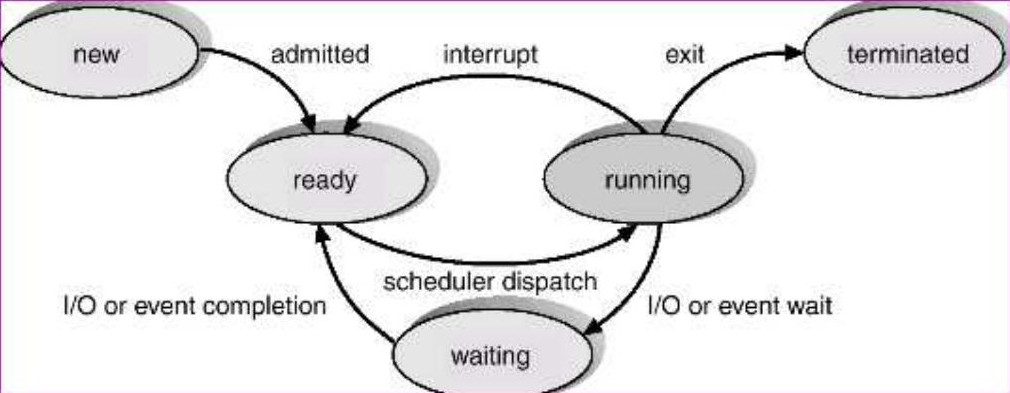
\includegraphics{8.6_1.jpg}}
    \caption{z prezentace IOS: Sprava procesu - stavovy diagram obecneho planovani procesu}
\end{figure}

\newpage

\textbf{Stavy planovani procesu v UNIXu:}
\begin{itemize}
    \item init - vytvoreny, neinicializovany,
    \item runnable - pripraven bezet,
    \item running - proces bezi (pridelen procesor), v pripade preempce (proces se vzda CPU) - jde do runnable,
    \item sleeping - proces pozada o I/O ci sync akci (ceka na dokonce operace), po realizaci bude runnable
    \item suspended - pomoci signalu SIGSTOP muze byt proces zmrazen a ceka ceka na rozmrazeni (signal SIGCONT),
    \item zombified - ukonceni procesu a prechod do stavu zombie (matoha), proces skoncil, odebrany vsechny zdroje, pouze o nem zustava zaznam v tabulce procesu (zde je jeho navratovy kod dokud si ho nekdo neprevezme) \\
\end{itemize}

% obrazek 6/38, sprava procesu
\begin{figure} [ht]
    \centering
    \scalebox{2}{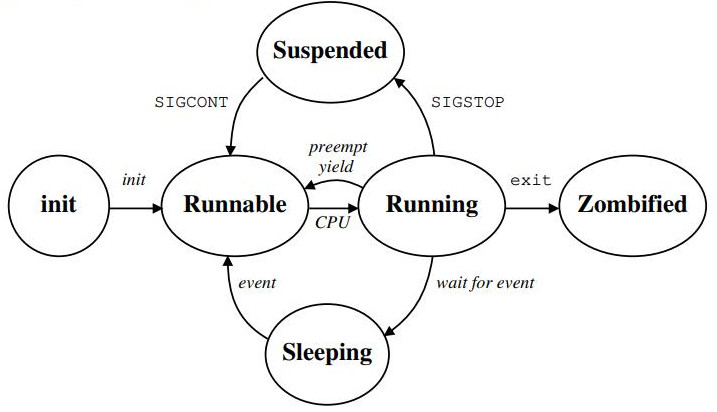
\includegraphics{8.6_2.jpg}}
    \caption{z prezentace IOS: Sprava procesu - stavovy diagram planovani procesu v UNIXu}
\end{figure}

OS s procesem pracuje tak, ze je reprezentovan pomoci struktury PCB (process control block), nekdy take task control block ci task struct. \\

\textbf{PCB zahrnuje (primo / formou odkazu):}
\begin{itemize}
    \item identifikatory spojene s procesem,
    \item stav planovani,
    \item obsah registru (v okamziku kdy je pozastaven),
    \item planovaci informace (priorita, ukazatele na planovaci fronty, ..),
    \item informace spojene se spravou pameti (tabulky stranek pri pouziti strankovaci pameti),
    \item informace spojene s uctovanim (sumarizuje informace o behu procesu - spotreba CPU, ..),
    \item informace o vyuziti I/O zdroju (otevrene soubory, tabulka popisovacu, ..) \\
\end{itemize}

PCB muze byt bud jedna struktura nebo muze byt rozdeleno na nekolik casti. \\

\subsection{Casti procesu v pameti v UNIXu}
Prvni soucast pameti vyuzite procesem je \textbf{uzivatelsky adresovy prostor} (user address space) - je pristupny procesu (muze z teto casti pameti cist/psat), obsahuje:
\begin{itemize}
    \item kod (ktery je rizen, code area/text segment),
    \item data (ne/inicializovana, hromada, alokovana pamet),
    \item zasobnik,
    \item soukroma data sdilenych knihoven, sdilene knihovny ci sdilena pamet \\
\end{itemize}

Dalsi cast informaci o procesech byva v nekterych pripadech - ne vzdy umistena v \textbf{uzivatelske oblasti} (napr. linux tento koncept nepouziva - vse ma v tabulce procesu):
\begin{itemize}
    \item ulozena pro kazdy proces v casti uzivatelskeho adresoveho prostoru, ktera neni pristupna procesu ,
    \item je to pristupne jadru,
    \item u kazdeho procesu si v teto casti uklada informace o procesu je tam:
    \item cast PCB, ktera je pouzivana zejmena za behu procesu,
    \item PID, UID, EID, GID, EGID, PPID (identifikator rodice),
    \item obsah registru,
    \item deskriptory souboru (informace o tom, ktere otevreni souboru reprezentuje stdin, stdout),
    \item obsluzne funkce signalu (funkce, ktere se budou volat pro obsluhu signalu),
    \item uctovani,
    \item pracovni, korenovy adresar \\
\end{itemize}

\textbf{Dalsi zaznamy jsou v tabulce procesu:}
\begin{itemize}
    \item ulozeno trvale v jadru,
    \item informace o procesu, ktere jsou dulezite i kdyz proces nebezi:
    \item PID, PPID, UID, EID, ...,
    \item stav planovani,
    \item udalost, na kterou proces ceka,
    \item planovaci informace (pro planovac pri rozhodovani ktery proces dal pobezi ci ne - priorita, spotreba casu, ..),
    \item cekajici signaly (signaly, kt. mohou prijit, i kdyz proces nebezi),
    \item odkaz na tabulky dat reprezentujici rozlozeni procesu, dat, kodu, zasobniku, .. \\
\end{itemize}

\newpage

Pote jsou jeste zaznamy v \textbf{tabulce pametovych regionu:}
\begin{itemize}
    \item jak je rozdelen uzivatelsky adresovy prostor na regiony (= souvisly kus pameti pouzity za urcity region, kod, zasobnik, ..),
    \item velikost techto regionu,
    \item globalni tabulka regionu (odkaz z teto na lokalni tabulky regionu),
    \item regiony byvaji cleneny na stranky (tabulky stranek) \\
\end{itemize}

\textbf{definice:} \\[0.5em]
\textit{logicky adresovy prostor} - rozsah vsech logickych adres, ktere se mapuji do fyzicke pameti \\[0.2em]
\textit{zasobnik jadra} je separatni zasobnik nekdy pouzivan pro ukladani rozpracovanych funkci jadro v okamziku kdy jadro provadi sluzbu pro dany proces \\

\subsection{Kontext procesu}
Je jine oznaceni pro \textbf{stav procesu}. Rozlisujeme:
\begin{itemize}
    \item uzivatelsky kontext - cast stavu procesu popisujici cast pameti dostupnou procesu samotnemu (kod, zasobnik, data),
    \item registrovy kontext,
    \item systemovy kontext - cast stavu procesu nedostupna samotnemu procesu (uzivatelska oblast, polozky tabulky procesu, pametove regiony,..) \\
\end{itemize}

\newpage

\subsection{Systemova volani nad procesy UNIXu}
= standardni POSIXova volani:
\begin{itemize}
    \item fork, exec, exit, wait, waitpid,
    \item kill, signal - synchronizace,
    \item getpid, getppid - ziskavani identifikatoru, ... \\
\end{itemize}

\textbf{Identifikatory spojene s procesy v UNIXu:}
\begin{itemize}
    \item identifikace procesu PID (vlastni identifikator procesu),
    \item identifikace predka PPID (proces, ktery dany proces vytvoril, rodic),
    \item realny-skutecny uzivatel, skupina uzivatelu, ktery proces spusitl - GID, GID,
    \item efektivni uzivatel ci skupina - EUID, EGID (viz. SUID, SGID v x.x),
    \item ulozene EUID a EGID - procesu umoznuji docasne se zbavit vysokych prav, ktere ziskal (proces se dobrovolne vzda vyssich prav - ulozi se a pobezi s beznymi pravi - v okamziku provadeni kritickych operaci si prava zase navysi -- ochrana pred chybami v programech),
    \item v linuxu FSUID, FSGID (file system UID/GID - oddelena zvysena privilegia pro praci s filesystemu),
    \item PGID, SID (process group identifier, session identifier - skupina procesu ci sezeni, do kterych proces patri) \\
\end{itemize}

\textbf{definice:} \\[0.5em]
\textit{sezeni} je skupina skupin procesu vytvarejici se typicky pri praci s terminaly \\

\subsection{Vytvareni procesu}
Procesy v UNIXu vznikaji \textbf{volanim sluzby fork}. Fork je volani, ktere se \textbf{zavola jednou}, pokud nedojde k chybe, tak \textbf{skonci 2x}. Na zaklade volani fork vznika \textbf{vztah rodic-potomek (parent-child) a hierarchie procesu}. Vysledkem forku je totiz \textbf{duplikace procesu}. Vznika takrka identicka kopie potomka, ktery dedi:
\begin{itemize}
    \item ridici kod, data, zasobnik, sdilenou pamet, otevrene soubory, obsluhu signalu, vetsinu synchronizacnich prostredku, ..
    \item pro efektivitu pouziva pro praci s pameti copy-on-write
    \item kopie se lisi v navratovem kodu fork, identifikatorech, udajich spojenych s planovanim a uctovanim, nededi se cekajici signaly, souborove zamky a nektere dalsi zdroje ci nastaveni .. \\
\end{itemize}

\textbf{Navratove kody forku:}
\begin{itemize}
    \item 0 - fork se zdaril, if(pid==0) { kod pro potomka }
    \item -1 - fork se nezdaril, if(pid==-1) { kod rodice }
    \item cokoli jineho (PID potomka) - else { kod pro rodice } \\
\end{itemize}

\newpage

\subsection{Hierarchie procesu v UNIXu}
Prvnim procesem, ktery vznika a vyvtvari ho jadro je \textbf{proces init s PID=1} (aktualni novejsi implementace je pojmenovana jako systemd - prikaz pstree). Tento proces je \textbf{predkem vsech ostatnich uzivatelskych procesu}. \textbf{PPID initu je 0}.

Existji take procesy jadra (kernel threads/processes), jejich init predkem neni:
\begin{itemize}
    \item jejich kod je soucasti jadra,
    \item vyskytuje se i proces s PID=0, vznika uplne jako prvni, podili se na inicializaci jadra, nasledne se meni na swapper (pokud je na systemu pouzit) nebo na cekaci smycku ci je to pouzivano jako procesova obalka pro vlakna jadra (na linuxu se tento proces nevypisuje) \\
\end{itemize}

Init se podili na \textbf{inicializaci systemu}, pote \textbf{prebira navratove kody procesu, ktere skonci, ale ktere osirely driv nez skoncily} (tedy rodic skonci driv nez potomek) - teoreticky by byl zombie procesem do nekonecna, proto init prebira jeho navratovy kod a umozni mu odchod ze systemu.

\textbf{definice:} \\[0.5em]
\textit{swapper} je proces, ktery slouzi k tomu, ze v pripade akutniho nedostatku pameti nektere procesy pozastavi a zcela ulozi na disk (veskere casti pameti zabirane procesem) \\[0.2em]
\textit{kthread} je proces, na linuxu init pro procesy jadra, ma PID=2 \\

\textbf{linux:} \\[0.5em]
\textit{pstree} vypis stromu procesu \\

\subsection{Zmena programu -- exec}
Umoznuje v ramci existujiciho procesu vymenit "jeho vnitrnosti" - \textbf{zahodit existujici kod a nahradit ho kodem jinym}. Exec je funkce, ktera se \textbf{zavola jednou a neskonci vubec} (je v nejakem kodu, ten kod prestane bezet) pokud nedojde k chybe.

Pokud v procesu zavolam exec:
\begin{itemize}
    \item porad dedi radu rysu sveho predka,
    \item zustava mu rada zdroju a vazeb OS (identifikatory, otevrene soubory, ..),
    \item zanikaji vazby a zdroje vazane na puvodni ridici (obsluzne funkce signalu, sdilena pamet, pametove mapovane soubory, semafory).
\end{itemize}

Skupina funkci exec:
\begin{itemize}
    \item execve (zakladni volani), execl, execlp, execle, execv, ..
\end{itemize}

Pozn.: Ve Windows se procesy vytvari volanim CreateProcess( ... ), ktere zahrnuje funkcnost fort i exec. \\

\newpage

\subsection{Cekani na potomka - wait, waitpid}
Slouzi k tomu, aby mohl \textbf{rodic cekat (pasivne) na dokonceni cinnosti svymi potomky}.

Volani wait:
\begin{itemize}
    \item ceka na ukonceni 1 z potomku,
    \item vraci cislo potomku, ktery skoncil (pripadne -1 pokud prijde signal, ktery cekani prerusi nebo pokud cekame na potomka a zadneho nemame),
    \item muze to byt operace blokujici, pokud zadny z potomku jeste neskoncil, 
    \item pokud nektery potomek skoncil driv pred volanim wait, okamzite volani wait skonci a vrati se navratovy kod. \\
\end{itemize}

Volani waitpid:
\begin{itemize}
    \item umoznuje cekani na ukonceni urciteho potomka urcite skupiny dle PID
    \item umoznuje cekani i na pozastaveni ci probuzeni (SIGSTOP, SIGCON). \\
\end{itemize}

\subsection{Start systemu}
\begin{itemize}
    \item (nejprve) dostane se ke slovu firmware PC (UEFI/BIOS),
    \item nacteni a spusteni zavadece OS (nekdy se zavadecu pouziva nekolik, napr. BIOS vyuzival zakladni kod MBR - serie zavadecu),
    \item nactou se inicializacni funkce jadra a samotneho jadro, spusteni inicializacnich funkci,
    \item inicializacni funkce jadra vytvori proces 0, dalsi procesy jadra a proces init,
    \item proces init pokracuje v inicializaci systemy, spostu demony a procesy,
    \item v urcitem okamziku se z nej spusti procesy umoznujici prihlaseni v GUI (GDM, SDDM, LightDDM) bud z nich nebo s nim spolupracujici procesu se spousti procesy pro praci s X Windows,
    \item na konzolich se spusti getty (ctrl+alt+f1,f2,..) - umozni uzivateli zadat prihlasovaci jmeno, zmeni se na login, nacte od uzivatele heslo, pote se zmeni na shell, ze ktereho se spousti dalsi procesy, po ukonceni se opet spousti getty,
    \item proces init i po inicializaci nadale bezi, prebira navratove kody procesu, jejich rodic skoncil driv nez prislusny proces, take resi reinicializaci systemu (na prani uzivatele ci vypadek napajeni) \\
\end{itemize}

\textbf{definice:} \\[0.5em]
\textit{firmware} je program ulozeny v nevolatilnich pametech, provadejici kontrolu hadrware, pripadnou inicializaci hw  \\

\newpage

\subsection{Urovne behu}
System urovni behu byl zaveden jiz v UNIX System V. Rozlisuji se urovne behu 0-6: (nektere mely predpripraveny standardni vyznam, nektere si definoval administrator)
\begin{itemize}
    \item 0=halt - zastaveni systemu,
    \item 1=single user - jednouzivatelsky rezim, pouziva spravce systemu,
    \item 3-6=definovane rezimy adminem,
    \item 6=reboot - automaticke restartovani,
    \item s/S=jednouzivatelsky rezim - daji se zde ale definovat ruzne akce, ktere se maji provadet pri prepnuti do techto rezimu,
    \item je mozne zmenit urovne behu (rezimy) pomoci \textit{tellinit N}. \\
\end{itemize}

Konfigurace urovni behu:
\begin{itemize}
    \item v adresari /etc/rcX.d (X=uroven behu), jsou skripty spoustene pri vstupu do dane urovne,
    \item nejprve se volaji skripty zacinajici K v poradi danem cislem za tim K (volaji se s argumentem stop),
    \item pote se volaji skripty zacinajici S (volaji se s argumentem start),
    \item start, stop - definuje se co se ma spustit ci jak se co ma zastavit,
    \item v adresari /etc/init.d vytvorime skript, ktery pozadovanou sluzbu bude umet spoustet, na patricne misto K a S odkazu se vytvori symlink na pozadovany skript,
    \item skripty v inid.d typicky prijimaji parametry start, stop, reload, restart
    \item tyto skripty se nemusi volat pouze pri zmene urovne behu, ale je mozne je volat i rucne - z /etc/inid.d
    \item v souboru /etc/inittab je horni, hlavni uroven systemu, kde se popisuje napr. implicitni uroven behu ci jake urovne behu jsou podporovane \\
\end{itemize}

Existuji ruzne nove implementace procesu init - dnes nejbeznejsi je \textbf{systemd}:
\begin{itemize}
    \item zakladni urovne behu jsou nahrazeny jednotky (units), ktere maji ruzne typy (targets, services, ..),
    \item spousti inicializacni jednotky paralelne na zaklade jejich zavislosti (= vyhodou je, ze inicializace systemu je mozne provadet paralelne, zatimco init se dela sekvencne),
    \item emuluji se urovne behu (zpetna kompatibilita),
    \item uzitecne jsou adresare /lib/systemd ci /usr/lib/systemd, .. (podrobne informace o systemd) \\ 
\end{itemize}

\newpage

\subsection{Planovani procesu} \label{planovani}
Procesy planuje planovac.

Rozlisujeme 2 \textbf{planovaci algoritmy} (definice viz. \ref{ne-preemtive}):
\begin{itemize}
    \item nepreemtivni planovani (typicky I/O operace, konec - volani exit, vzda se CPU - yield),
    \item preemtivni planovani (typicky preruseni od casovace, muze jit i o jine, treba od disku) \\
\end{itemize}

Rozlisujeme \textbf{3 "typy" planovani}:
\begin{itemize}
    \item dlouhodobe planovani - ktere ulohy budou pripusteny do systemu,
    \item strednedobe planovani - procesy maji pamet / nemaji pamet - jedna se o system swapovani,
    \item kratkodobe planovani - procesy maji pamet - prepinani mezi ulohami \\
\end{itemize}

\textbf{System swapovani} (= strednedobe planovani):
\begin{itemize}
    \item v pripade nedostatku pameti nektere procesy pozastavi, odebere jim veskerou pamet a ulozi je na disk,
    \item tyto procesy jsou vyrazeny z planovani (nemaji pamet - nemohou bezet),
    \item pri zadosti o spusteni ulohy uloha pak nebude spustena ihned, ale system ceka na uvolneni systemovych zdroju (sluzba ceka ve fronte) - pote uz se jedna dlouhodobe planovani (rozhoduje se o tom, ktere ulohy budou vubec pripusteny do systemu) \\
\end{itemize}

\textbf{definice:} \\[0.5em]
\textit{planovac} rozhoduje ktery proces ci procesy pobezi a pripadne jak dlouho \\[0.2em]
\textit{systemy s neepremtivnim planovanim} = systemy s kooperovanym planovanim (procesy musi spolupracovat, kooperovat) \\

\subsection{Prepnuti kontextu (procesu)}
Prepnuti kontextu na prikladu - dispecer na zaklade rozhodnuti planovace prepina mezi procesem A a B:
\begin{itemize}
    \item bude muset uchovat stav registru (nekterych, ale vcetne ridicich registru) procesu A do PCB (nebo task struct v linuxu),
    \item dojde k uprave nekterych ridicich struktur v jadre (uprava planovacich struktur, uctovacich struktur, ..),
    \item obnova ulozenych hodnot registru procesu B,
    \item dojde k predani rizeni proceu na adresu, kde bylo drive preruseno provadeni procesu B,
    \item tato akce se musi provadet v rezimu jadra \\
\end{itemize}

Neuklada se a neobnovuje cely stav procesu (pri pozastaveni procesu neni nutne na disk ukladat obsah pameti, ukladaji se pouze registry).

Presto prepnuti muze trvat \textbf{radove stovky/tisice instrukci} - jadra umoznuji interval v jakem prichazeji preruseni z casovace - je treba si dat pozor, aby ten interval nebyl prilis kratky, protoze zacne pote prevazovat rezie systemu nad uzitecnym behem (neustale ukladani a obnovovani obsahu registru).

\newpage

\section{}
\textbf{Devata prednaska:} Dokonceni spravy procesu.

\subsection{Kratke planovaci algoritmy}
\subsubsection{FCFS}
\begin{itemize}
    \item first come, first served,
    \item planovaci algoritmus zalozeny na jednoduche FIFO fronte,
    \item proces, ktery nove vznikne nebo je uvolnen z cekani na nejake operaci (I/O, sync, ..), pripadne proces, ktery se vzda CPU,
    \item se zaradi na konec fronty,
    \item procesy, ktere pobezi se vybiraji ze zacatku fronty,
    \item jedna se o nepreemtivni algoritmus (prepnuti kontextu dojde pokud se bezici proces vzda CPU ci zavola sluzbu jadra) \\
\end{itemize}

\subsubsection{Round-robin}
\begin{itemize}
    \item preemtivni obdoba FCFS,
    \item pracuje podobne jako FCFS,
    \item kazdy proces ma prideleno nejake casove kvantum,
    \item jakmile je mu pridelen CPU, proces bezi a pobezi nanejvys po dobu casoveho kvanta,
    \item po vyprseni casu je procesu odebran CPU a je zarazen na konec fronty,
    \item CPU se prideli procesu ze zacatku fronty \\
\end{itemize}

\subsubsection{SJF}
\begin{itemize}
    \item shortest job first,
    \item nejprve se provede nejkratsi uloha,
    \item algoritmus prideluje CPU tomu procesu, ktery aktualne deklaruje nejkratsi dobu pro svuj dalsi beh na CPU, po ktery nebude zadat o zadne I/O operace (tzv. CPU burst),
    \item beh uloh se deli na vypocetni prace (CPU burst) a pote na periody, kdy se komunikuje s periferiemi (disky, site,..),
    \item nepreemtivni algoritmus (neprerusuje proces pred dokoncenim jeho aktualni vypocetni faze),
    \item statisticky minimalizuje prumernou dobu cekani a zvysuje propustnost systemu,
    \item je nutne dopredu znat dobu behu procesu na CPU v jejich jednotlivych vypocetnich fazich, ci musi tu byt moznost tyto doby rozumne odhadnout (na zaklade predchoziho chovani techto uloh),
    \item dava smysl pro opakovane provadene ulohy, 
    \item pouziva se zejmena v davkovych (specializovancyh) systemech,
    \item nevyhodou algoritmus je starnuti (hladoveni, starvation) - ke starnuti dochazi pri cekani na nejake zdroje (CPU, zamek, ..) je situace, kdy nektery proces, ktery o ten zdroj zada, na nej ceka bez zaruky, ze nej nekdy ziska,
    \item pokud nejaky proces deklaruje delku CPU burst a v systemu budou neustale kratsi procesy s touto delkou, tyto procesy ho budou neustale predbihat (nikdy se tak k CPU nedostane) \\
\end{itemize}

\subsubsection{SRT}
\begin{itemize}
    \item shortest remaining time,
    \item preemtivni obdoba SJF,
    \item je zde prevence pri vzniku ci uvolneni procesu z cekani (kdyz se uvolni novy proces a deklaruje kratsi vypocetni fazi nez ten, ktery dosud bezel - muze byt provaden on), \\
\end{itemize}

\subsubsection{Viceurovnove planovani}
\begin{itemize}
    \item procesy rozdeleny do ruznych skupin (typicky dle priority, ale ne nutne - napr. dle typu procesu),
    \item kazda skupina procesu muze pouzivat jiny dilci planovaci algoritmus (FSFS, round-robin, SJF, ..) s ruznymi parametry,
    \item krome toho mame dalsi ("hlavni") algoritmus, ktery rozhoduje, ktera skupina procesu dostane CPU cas - casto jednoduse na zaklade priorit skupin,
    \item pote je dalsi planovaci algoritmus, ktery planuje mezi skupinami \\
\end{itemize}

\subsubsection{Viucerovnove planovani se zpetnou vazbou}
\begin{itemize}
    \item skupiny procesy jsou rozdeleny dle priorit,
    \item proces, ktery se stane nove pripravenym bezet (nove vznikne, je uvolnen z cekani, ..) je zarazen do skupiny procesu s nejvyssi prioritou.
    \item v teto skupine bezi a postupne klesa do nizsich priorit,
    \item az spadne do nejnizsi urovne (planovan round-robin),
    \item pouzivaji se varianty, kdy proces ma prednastavenou statickou prioritou a zaradi se do planovaci urovne teto priority, a pote ma i dynamickou prioritu, ktera se muze zvysovat i snizovat, typicky se priority meni tak, ze pokud nejaky proces spotrebovava mnoho CPU casu - priorita se snizi, proces ceka na mnoho I/O operaci - priorita se zvysi,
    \item cilem je zajistit rychlou reakci interaktivnich procesu, \\
\end{itemize}

\textbf{definice:} \\[0.5em]
\textit{interaktivni procesy} jsou procesy komunikujici s uzivatelem \\ 

\subsection{Planovac v Linuxu (od verze 2.6.23)}
Pouziva se \textbf{viceurovnove prioritni planovani se 100 zakladnimi statickymi prioritnimi urovnemi}:
\begin{itemize}
    \item priority 1-99 jsou vyhrazeny pro procesy realneho casu (algoritmy FCFS s preemci na zaklade priorit nebo round-robin),
    \item priorita 0 jsou bezne procesy planovane CFS planovacem,
    \item v ramci urovne 0 se pouzivaji podurovne v rozmezi -20 az 19, nejvyssi poduroven je -20 (je mozne bezne uzivatelsky nastavovat prikazy nice/renice),
    \item v ramci urovne 0 se rozlisuji 3 typu procesu (bezne, davkove a idle procesy),
    \item zakladni prioritni uroven (RT proces v 1-99, bezny proces) a typ planovani (round-robin, FCFS, ..) je mozne nastavit pomoci sluzby sched\_setscheduler,
    \item pozdeji pridano planovani pro sporadicke periodicke ulohy - zalozeno na strategii earliest deadline first (prezvato z RT OS) \\
\end{itemize}

\textbf{definice:} \\[0.5em]
\textit{FCFS s preemci na zaklade priorit} - pokud behem behu procesu dobehne I/O operace ci sync operace, ktera zpusobi proveditelnost procesu s vyssi prioritou, dojde k prepnuti kontextu  (nedochazi k prepnuti kontextu na zaklade casovych kvant s procesy s stejnou prioritou) \\[0.2em]
\textit{davkove procesy} maji mirnou penalizaci s hlediska priorit, maji ale delsi kvantum \\[0.2em]
\textit{idle} maji nizkou prioritu, procesy, u ktery se predpoklada, ze se dostanou ke slovu az v okamzik, kdyz v systemu nic uzitecnejsiho neni \\[0.2em]
\textit{sporadicke periodicke ulohy} jsou ulohy, ktere bezi, maji periodicke vypocetni faze (ocekavana faze - zname dobu jak dlouho trvaji + mame casovy limit, dokdy se maji vypocty provest), ktere se provadeji cas od casu \\[0.2em]

\subsection{Completely Fair Scheduler}
Neboli CFS planovac:
\begin{itemize}
    \item snazi se explicitne kazdemu procesu poskytnout odpovidajici procento strojoveho casu s ohledem na jeho priority (4 procesy, stejna priorita - vsichni 25 procent CPU),
    \item u kazdeho procesu si vede udaje o tom, kolik virtualniho CPU casu uz ten proces na CPU stravil,
    \item vede si udaj o minimalnim stravenem CPU case (dava nove pripravenym procesum),
    \item procesy udrzuje ve vyhledavaci strukture red-black tree podle vyuziteho CPU casu,
    \item pri rozhodovani, ktery proces pobezi, z strukturu vezme ten, ktery aktualne stravil nejmene casu na CPU,
    \item proces necha bezet po casove kvantum, ktere spocita na zaklade priorit,
    \item virtualni procesorovy cas - situace: 2 procesy bezici cely den (kazdy pul dne), prijde novy proces, fyzicky na CPU bezel 0s (nejvyssi priorita, bezel by pul dne a ty 2 by byly off), proto virtualni CPU cas - novy proces dostane cas mensi nez minimalni straveny cas vsemi procesy (ne 0),
    \item algoritmus ma podporu pro skupinova planovani, umi rozdelovat cas spravedlive pro skupiny procesu (spoustene z ruznych terminalu, od ruznych uzivatelu, ..) \\
\end{itemize}

\subsection{Planovani ve Windows NT a novejsich}
\begin{itemize}
    \item Pouziva se viceurovnove prioritni planovani se zpetnou vazbou na zaklade interaktivity:
    \item 32 prioritnich urovni, 0 - nulovani volnych stranek pameti (aby pres ne se nedostaly informace od jednoho uzivatel k jinemu), 1 - 15 bezne procesy, 16 - 31 procesy realneho casu,
    \item zakladni priorita procesu je dana kombinaci planovaci tridy a planovaci urovne (v ramci tridy),
    \item priorita se dynamicky snizuje ci snizuje:
    \item zvysi se priorita procesu spojene s oknem, ktere je v popredi,
    \item zvysi se priorita procesu spojene s oknem, do ktere prichazi vstupni zpravy (mys, casovac, klavesnice, ..),
    \item zvysuje se priorita procesu uvolnenych z cekani (I/O operace),
    \item zvysena priorita se po kazdem vycerpani kvanta snizu o jedno uroven (az do dosazeni zakladni priority) \\
\end{itemize}

\subsection{Inverze priorit}
Jedna se o \textbf{nezadouci problem}, ktery je nutne resit:
\begin{itemize}
    \item jedna se o situaci, kdy v OS mame ruzne prioritni procesy, malo prioritni proces si naalokuje si nejaky zdroj, zamkne si pristup k nejakemu sdilenemu sdroji (soubor, adresa v pameti, sitovy port, ..),
    \item viceprioritni procesy tyto procesy predbihaji, 
    \item nizkoprioritni proces se cas od casu dostane ke slovu, provede par instrukci, musi cekat,
    \item (ma naalokovany zdroj, chce s nim neco provest, to ale trva dlouho, protoze ho porad nekdo predbiha),
    \item muze nastat, ze nektery z viceprioritnich procesu potrebuje prave ten zdroj, ktery si zamknul tento nizkoprioritni proces,
    \item vysoceprioritni proces bude muset tak cekat - virtualne se zvysi (rapidne) priorita nizkoprioritniho procesu (= je to vedlejsi efekt, prioritu ma porad stejnou!),
    \item v systemu je mozne mit stredneprioritni procesy, ktere tento zdroj nepotrebuji, ty budou predbihat dale nizkoprioritni proces,
    \item vysokoprioritni proces musi cekat, zatimco stredneprioritni a nizkoprioritni maji najednou "vyssi prioritu",
    \item tento jev muze a nemusi vadit - muze zpusobit snizenou odezvu systemu, nicmene muzou se zablokovat i nektere kriticke procesy realneho casu (ovladani hardware, ..) \\
\end{itemize}

\textbf{Moznosti reseni inverze priorit:}
\begin{itemize}
    \item prioritni strop - priority ceiling - procesy v kriticke sekci ziskavaji nejvyssi prioritu,
    \item priority inheritance - procesy v kriticke sekci, ktery blokuje vyse prioritni procesy po dobu behu v kriticke sekci dedi prioritu cekajiciho procesu (s nejvyssi prioritou),
    \item na jednoprocesorovych systemech se pouziva technika, kdy po dobu behu v kriticke sekci se zakaze preruseni \\
\end{itemize}

Dalsi komplikace behem planovani:
\begin{itemize}
    \item viceprocesorove systemy - nutne vyvazovat vykon (aby na jednom jadru CPU nebezely 4 procesy a na zbytku 0), respektovat obsah cache CPU, lokalitu pameti (neuniformni pristup do pameti)
    \item hard real-time systemy - nutnost zajistit garantovanou odezvu nekterych akci \\
\end{itemize}

\textbf{definice:} \\[0.5em]
\textit{kriticka sekce} je sekce v kodu, kde se pracuje vylucnym zpusobem se sdilenymi prostredky \\[0.2em]
\textit{neuniformni pristup do pameti} - pamet je delena na pametove jednotky, kazda pripojena k jinemu CPU, ale vsechny procesy mohou pristupovat do vsech pametovych jednotek (za ruznou dobu) \\

\subsection{Vlakna, ulohy, skupiny procesu}
Vlakna, neboli threads:
\begin{itemize}
    \item oznacovana jako odlehcene procesy (LWP - lightweight process),
    \item vypocty (odpovidaji vlaknum) bezici paralelne v jednom procesum,
    \item vlakna maji vlastni obsah registru, vlastni zasobnik,
    \item vsechna vlakna sdili stejny ridici kod, data, dalsi zdroje (otevrene soubory, signaly),
    \item vyhody: rychleji se spousti, prepina, efektivnejsi prace (dle systemu - v UNIXu diky fork rozdil mezi vlakny a procesy je mensi nez jinych OS), .. \\
\end{itemize}

\newpage

\subsection{Ulohy, skupiny procesu, sezeni}
\textbf{Uloha (job)} se poji se shellem, je skupina skupina paralelne bezicich procesu spustenych jednim prikazem, prikazy propojene do kolony (p1 | p2 | p3 - pipeline). \\

\textbf{Skupina procesu (process group) v UNIXu:}
\begin{itemize}
    \item mnozina procesu paralelne bezicich, se kterymi je mozne provadet operace jako s celkem,
    \item skupine je mozne poslat signal jako 1 jednotce,
    \item predek take muze cekat na libovolneho potomka z urcite skupiny,
    \item kazdy proces prave v 1 skupine procesu, po vytvoreni vzdy je to skupina jeho predka,
    \item skupina muze a nemusi mit vedouciho - jeji prvni proces, dokud neskonci (pokud skonci - skupina bez vedouciho),
    \item skupina je identifikovana vedoucim skupiny, pokud vedouci skupiny skonci, neni mozne jeho cislo recyklovat a pouzit pro ID skupiny \\
\end{itemize}

\textbf{Sezeni v UNIXu:}
\begin{itemize}
    \item mnozina skupin procesu,
    \item kazda skupina procesu je v jednom sezeni,
    \item sezeni muze a nemusi mit vedouciho,
    \item muze mit ridici terminal (/dev/tty),
    \item v ramci sezeni plati, ze jedna skupina je na popredi (cte z terminalu), ostatni jsou na pozadi,
    \item pokud terminal konci, signalem je SIGHUP, informovan je vedouci sezeni (typicky shell), standardtne se vsem procesum, na ktere nebyl uzit prikaz nohup/disown, posle navic SIGHUP, pokud jsou procesy pozastaveny, tak posle signal SIGCONT \\
\end{itemize}

\newpage

\subsection{Komunikace procesu}
Pouziva se \textbf{IPC - inter-process communication:}
\begin{itemize}
    \item signaly (umoznuji zasilat mezi CPU informace pomoci cisla),
    \item roury,
    \item zasilani zprav (umoznuji posilat retezcova data),
    \item sdilena pamet,
    \item sockety,
    \item RPC (remote procedure call), ... \\
\end{itemize}

\subsection{Signaly}
V zakladni verzi je cislo (int), ktere je procesu zaslano prostrednictvim pro to zvlast definovaneho rozhrani (= signaly v OS, nikoli na vodicich). Jsou generovany:
\begin{itemize}
    \item pri chybach (aritemticka chyba, chyby sbernic, ..),
    \item externich udalostech (dostupnost I/O, vyprseni casovace, ..),
    \item na zadost procesu - IPC (meziprocesova komunikace, procesy si mohou navzajem posilat singnaly, ale jadru signal nelze zaslat - jadro neni proces),
    \item vznikaji obvykle asynchronne k cinnosti programu (program neco provadi, nezavisle na tom co provadi v okamziku ktery nelze predpovedet prijde signal) \\
\end{itemize}

Je nutne peclive zvazovat obsluhu signalu, aby aplikaci \textbf{signal neshodil, vznikaji chyby, ktere se objevuji jen zridka} (spatne ladeni, tzv. race conditions) - vede to na vyuzivani technik pro \textbf{pokrocile testovani} (vkladani sumu - umele v nahodnych okamzicich se snazime programy zpozdit, enumerace prolozeni akci programu), \textbf{nastroje pro verifikaci s formalnimi zaklady} (staticka analyza, model checking). \\

Mezi bezne pouzivane signaly patri:
\begin{itemize}
    \item SIGHUP - odpojeni, ukonceni terminalu,
    \item SIGINT - preruseni z klavesnice (Ctrl+C),
    \item SIGKILL - signal c.9, tvrde ukonceni
    \item SIGSEV (mimo pridelenou pamet - spatny ukazatel),SIGBUS - chybna prace s pameti,
    \item SIGPIPE - zapis do roury bez ctenare,
    \item SIALRM - signal od casovace,
    \item SIGTERM - mekke ukonceni (lze vyvratit),
    \item SIGUSR1, SIGUSR2 - uzivatelske signaly (uzivatel si je muze nadefinovat)
    \item SIGCHLD - pozastaveni ci ukonceni potomka,
    \item SIGCONT - dochazi pri uvolneni z cekani,
    \item SIGSTOP, SIGSTP (Ctrl+Z) - tvrde / mekke pozastaveni,
    \item dalsi viz man 7 signal \\
\end{itemize}

\textbf{definice:}
\textit{race conditions} jsou casove zavisle chyby (zavisi na tom, jak se v case na sobe nakladaji paralelni akce) \\

\subsubsection{Predefinovani obsluhy signalu}
Mezi implicitni reakce na signal patri \textbf{ukonceni procesu} (pripadne s generovani core dump), \textbf{ignorovani signalu, zmrazeni ci rozmrazeni procesu}. 

Predefinovat obsluhu lze u vsech signalu \textbf{mimo SIGKILL, SIGSTOP}. U SIGCONT vzdy dojde k odblokovani procesu (a nasledne se provede preddefinovana akce). \\

Vlastni predefinovani obsluhy:
\begin{itemize}
    \item pouziji se funkce signal (zakladni - jaky signal chci obsluhovat a jakou funkci, funkce ma jediny parametr - cislo signalu)
    \item nebo sigaction (urci se jaka funkce bude obsluzna, moznst nastaveni blokovani signalu behem obsluhy, dalsi specialni rezimy, .. ) 
    \item vice viz. man signal nebo man sigaction \\
\end{itemize}

Prednastavene konstanty:
\begin{itemize}
    \item SIG\_DFL - prednastaveny signal ma byt obsluhovan implicitnim zpusobem
    \item SIG\_IGN - signal ma byt ignorovan \\
\end{itemize}

Z obsluzne funkce je mozne volat pouze bezpecne knihovni funkce. (viz. man 7 signal - na konci seznam funkci, ktere se mohou pouzit pri obsluze funkci) \\

\subsubsection{Blokovani signalu}
Je vhodne nastavit masku blokovani signalu, volani:
\begin{itemize}
    \item sigprocmask (rekneme jake nastaveni signalu menime),
    \item pomoci SIG\_BLOCK (co chceme blokovat), SIG\_UNBLOCK (odblokovat), SIG\_SETMASK (natvrdo nastavit masku blokovanych signalu). \\
\end{itemize}

Blokovani se resi pomoci \textbf{bitovych masek}, ktere jsou typu sigset\_t. K vytvareni masek je mozne pouzit preddefinovana makra sigemptyset, sigfillset, segaddset, sigdelset. Nelze blokovat signaly \textbf{SIGKILL, SIGSTOP, SIGCONT}.

\textbf{Nastaveni blokovani se dedi blokovani potomku} (proces si nastavi blokovani - fork - dedi to i potomci, pri execu obsluzne funkce zanikaji). Pokud chceme zjistit, zda nejake signaly cekaji, zavolame sigpending (preda se ukazatel na masku signalu). Pokud nejaky signal je zablokovan, ale prijde vicekrat, zapamtuje se jeho \textbf{vyskyt pouze 1x}. (neplati pro realtime signaly)

\subsubsection{Zasilani signalu}
Slouzi k tomu volani kill (s parametry pid - komu chceme signal poslat a cislo signalu, ktery zasilame). Umoznuje zasilat signaly:
\begin{itemize}
    \item jednomu konkrektnimu procesu (pid kladne),
    \item skupine procesu (0 - ve skupine, ve ktere proces je),
    \item vsem procesum, kterym proces muze signal poslat (pid = -1, nebo zapornejsi cislo - posle se dane skupine [-10] = vsem v skupine 10). \\
\end{itemize}

Aby mohl proces zaslat signal jinemu procesu, musi odpovidat \textbf{jeho UID, EUID ci saved set-user-ID ciloveho procesu} (nelze posilat signaly nekomu jinemu), pripadne se musi jednat o privilegovaneho odesilatele (napr. EUID=0, nebo CAP\_KILL).

Muze se pouzit i sigqueue pro volani s realtime signaly.

\subsubsection{Cekani na signal}
Meli bychom na signaly cekat \textbf{pasivne} (nikoli se aktivne neustale dokola ptat, zda signal uz prisel). Budto:
\begin{itemize}
    \item jednoduche cekani pause,
    \item obvykle lepsi zabezpecene cekani sigsuspend - je mozne specifikovat masku signalu, ktere maji byt blokovany po dobu cekani a atomicky prepnout mezi signaly jsou blokovany do zacatku cekani a od zacatku cekani (muze se stat, ze probehne test, zda prisel nejaky signal a zjisti se, ze neprisel - zacne se cekat a prijde mezi testem a zacatkem cekani - cekani do nekonecna) \\
\end{itemize}

\newpage

\section{}
\textbf{Desata prednaska:} Nove tema - synchronizace procesu.
\subsection{Synchronizace procesu}
Synchronizace slouzi k tomu, aby procesy si vzajemne \textbf{nekolidovali a nedochazelo v systemu k nekonzistentnim stavum (ci datum).} -- Aby pri behu procesu nedoslo ke nekonzistenci dat, pouziva se synchronizace procesu (zajistuje spravne poradi provadeni spolupracujicich procesu).

Kdyz jadro dava \textbf{casove kvantum nejakemu procesu, tak to znamena, ze dava procesu nejaky casovac}, a kdyz dobehne, \textbf{spusti se preruseni}.

\textbf{Race condition:} \\
Casove zavisla chyba, ci race condition nebo soubeh, chyba, ktera muze vzniknout pri pristupu ke sdilenym zdrojum, datum - vznika pri pristupu ke zdilenym zdrojum kvuli ruznemu poradi provadeni jednotlivych paralelnich vypoctu v systemu. \\

\subsection{Kriticke sekce}
Jsou \textbf{useky kodu napric ruznymi procesy}, ve kterych \textbf{nesmi dojit k prepnuti kontextu} (nebo v nich nesmi byt nekolik procesu zaroven), \textbf{aby nedoslo k chybe soubehu dat}. (napr. vice procesu pracuje se stejnymi [globalnimi] promennymi) V programu muze byt \textbf{vice} kritickych sekci.

Problemem kriticke sekce rozumime \textbf{problem zajisteni konkretni synchronizae procesu na mnozine sdilenych kritickych sekci}, coz zahrnuje:
\begin{itemize}
    \item vzajemne vylouceni - nanejvys 1 (ci k) procesu muze do kriticke sekce vstouput (nebo: nanejvys 1 proces je v danem okamziku v dane mnozine sdilenych kritickych sekci).
    \item dostupnost kritickych sekci:
    \item pokud je kriticka sekce volna, chceme do ni vstouput (nebo: opakovane volna v alespon urcitych okamzicich, proces nemuze neomezene cekat na pristup k ni),
    \item je potreba se totiz vyhnout:
    \begin{itemize}
        \item uvaznuti (deadlock, viz nize a pozdeji),
        \item blokovani (situace, kdy sdileny prostredek je volny, proces na nej ale musi dlouho cekat),
        \item starnuti (hladoveni, proces se snazi vstoupit do kriticke sekce, ale nikdy k tomu nedojde, protoze ho planovac nikdy nevybere ve spravny okamzik). \\
    \end{itemize}
\end{itemize}

\newpage

\subsection{Problemy vznikajici na kriticke sekci}
Data race - \textbf{dochazi k zavodu mezi daty} - situace kdy jsou treba dva pristupy ke zdroji s vylucnym pristupem ze dvou procesu bez synchronizace, alespon jeden pristup je zapis. Jedna se o:
\begin{itemize}
    \item Uvaznuti (deadlock) pri pristupu ke zdrojum s vylucnym (omezenym) pristupem rozumime situaci, kdy kazdy proces z urcite mnoziny procesu je pozastaven a ceka na uvolneni zdroje s vylucnym (omezenym) pristupem vlastneneho nejakym procesem z dane mnoziny, ktery jediny muze teto zdroj uvolnit,
    \item Livelock - specialni pripad starnuti - dochazi k tomu s tim, ze procesy vykonavaji nejakou cinnost, ale nikdy se nedostanou k tomu, aby udelali co chteli (nikdy nedojde ke vstupu do kriticke sekce),
    \item Blokovani pri pristupu do kriticke sekce je situace, kdy proces, jenz zada o vstup do kriticke sekce musi cekat, prestoze je prestoze je kriticka sekce volna a ani o zadnou z dane mnoziny sdilenych kritickych sekci zadny dalsi proces nezada,
    \item Starnuti je situace, kdy proces ceka na podminku, ktera nemusi nastat - v pripade kriticke sekce je touto podminkou umozneni vstupu do kriticke sekce \\
\end{itemize}

\subsection{Zpusoby reseni problemu kriticke sekce}
Musi dojit k \textbf{vzajemnemu vylouceni} (nesmi dojit k data race) a musi zajistovat \textbf{dostupnost kriticke sekce} (minimalne nesmi dojit k deadlocku) a zaroven synchronizacni prostredky musi byt efektivni.

\textbf{Petersonuv algoritmus (kratky popis):}
\begin{itemize}
    \item omezen pro 2 procesy (existuji i rozsireni pro vice procesu),
    \item resi sync kritiske sekce bez hardwaru,
    \item nebere ohled na to, jaka ta kriticka sekce je,
    \item v kriticke sekci muze byt maximalne 1 proces,
    \item procesy o sobe vzajemne nevi (nevi co druhy proces dela, pouze vedi, ze druhy proce existuje),
    \item pracuje s sdilenymi polemi booleovskych promennych (init false, false) a sdilenou promennou turn = 0,
    \item pole nam rika, ktery z procesu chce pristoupit do kriticke sekce,
    \item turn nam rika, kdo je zrovna na tahu (pred vstupem do kriticke sekce),
    \item prvni proces chce pristoupit do kriticke sekce - nastavi turn na 1 - i (i je index v bool poli), na tahu je druhy proces,
    \item zacne se provadet prazdny cyklus (dokud je nastaven flag 1 - i a zaroven je na tahu ten druhy proces - cykli),
    \item proces 1 provede kritickou sekcu a nastavi svuj bool na false \\
\end{itemize}

\textbf{Bakery algoritmus L. Lamporta:}
\begin{itemize}
    \item vylouceni pro n procesu (n znam dopredu),
    \item prijdes do pekarstvi (nebo spis na postu), vezmete si listek s cislem a cekas, az na tebe dojde rada,
    \item pred vstupem do kriticke sekce ziiska proces pristupovy listek, jehoz hodnota je vetsi nez cisla pridelena jiz cekajicim procesum,
    \item pracuje s sdilenym booleovskym pole priznaku (jestli hledam hodnotu maximalniho ticketu), sdilenym int hodnoty ticketu a lokalnimi int hodnotami,
    \item v prvni fazi se snazi algoritmus zjistit, jake je nejvetsi cislo tiketu a pote si vzit ticket s hodnotou maximum+1 vice,
    \item dva (nebo) vice procesu muze mit stejnou hodnotu ticketu,
    \item pote se nastavi bool na false,
    \item ve druhe fazi proces ceka, az bude na nej rada,
    \item nejprve pockam, az jiny proces (od 0) dohleda svoje maximum,
    \item pote se ceka, az bude na me rada (ticket kladny, ostatni procesy nebudou chtit pristoupit do kriticke sekce),
    \item az proces projde do kriticke sekce, hodnota jeho ticketu se nastavi na 0,
    \item v okamziku, kdy maji procesy stejne cislo ticketu, prednost ma proces s nizsim cislem procesu (PID),
    \item jednim problemem algoritmu je neustale zvysovani cisel (nutnost si davat pozor na preteceni) \\
\end{itemize}

Ani jeden z predeslych algoritmu nemusi na dnesnich CPU fungovat, protoze jsou \textbf{silne zavisle na poradi pristupu do pameti}. \\

\newpage

\subsection{Vyuziti atomickych instrukci pro synchroniaci}
Pouzivaji se spise tyto instrukce. Jsou zalozeny na vyuziti instrukci, jejich atomicita je zajistena hw.

\textbf{TestAndSet:}
\begin{itemize}
    \item v intelu lock bts, atomicka instrukce,
    \item lze si ji predstavit jako funkci co vraci bool a potrebuje odkaz na typ target (bool),
    \item nejdriv si ulozi to co je v pameti do pomocne promenne,
    \item pote na misto pameti ulozi true, 
    \item vrati co tam bylo predtim (puvodni hodnotu),
    \item pri synchronizaci se to da vyuzit napriklad tak, 
    \item ze proces ceka, az na danem pametovem miste bude hodnota false,
    \item projde do kriticke sekce,
    \item nastavi promennou na false a muze do ni pristoupit nekdo jiny,
    \item kriticka sekce je chranena tzv. zamkem \\
\end{itemize}

\textbf{Swap:}
\begin{itemize}
    \item v intelu lock a xchg, atomicka instrukce,
    \item nic nevraci, vymeni atomicky hodnoty ve dvou mistech v pameti,
    \item pri syncu se da vyuzit tak, ze se zamkne kriticka sekce prohozenim hodnot dvou promennych,
    \item vstoupime do kriticke sekce, a pote zamek odemkneme \\
\end{itemize}

Uvedena reseni zahrnuji moznost \textbf{aktivniho cekani}, a proto se take oznacuji casto jako \textbf{spinlock} (neustale se toci dokola a ptaji se na platnost podminky). Obecne jsou prilis drahe - procesy provadeji neuzitecny kod, pouze berou CPU cas. 

Lze je vsak vyuzit \textbf{na kratkych, neblokujicich kritickych sekcich bez preemce} (tam kde neni prepnuti CPU).

Pristup do pameti (RAM) od CPU trva kolem 100-150 instrukci. Opakovany zapis sdileneho pametoveho miste je problematicky z hlediska \textbf{zajisteni konzistence cache v multicpu systemech} (zatezuje se sdilena pametova sbernice) - resenim je pri aktivnim cekani \textbf{pouze cist}.

\textbf{definice:} \\[0.5em]
\textit{atomicka instrukce} je instrukce, u ktere je garantovano, ze je atomicka \\[0.2em]
\textit{atomicita instrukce} zn., ze instrukce nemuze byt prerusena \\[0.2em]
\textit{prazdny while (sync)} - aktivni cekani \\

\newpage

\subsection{Semafory}
Synchronizacni nastroj nevyzadujici aktivni cekani (nebo alespon minimalizujici - muze se vyskytnout uvnitr implementace operaci nad semaforem). Jedna se o \textbf{celociselnou promennou prostupnout dvemi zakladnimi atomickymi operacemi} (hodnota = kolik procesu do nej jeste muze vstoupit):
\begin{itemize}
    \item lock - zamknuti semaforu, proces vstoupi do kriticke sekce a ostatni budou uspany,
    \item unlock - odemknuti semaforu - jine procesy se probudi a vstoupi do kriticke sekce. \\
\end{itemize}

Dale je mozne mit rozsireni semaforu o:
\begin{itemize}
    \item neblokujici zamknuti - pokud je mozne zamknout semafor, tak se to provede, jinak se nebude cekat a provede se jina akce,
    \item zamknuti s horni mezi na dobu cekani - maximalni cekaci doba (pote se proces probudi a bude delat neco jine),
    \item soucasne zamknuti vice semaforu \\
\end{itemize}

Zabezpecuje sdileny pristup do kriticke sekce tak, ze \textbf{cekajici procesy uspi} (misto aktivniho cekani) a po uvolneni jej opet probudi. (Pozn.: \textbf{poradi pristupu procesu neni garantovano} (tzn. po uspani procesu se netvori fronta, ale spise nejaka mnozina procesu))

Semantika celociselne promenne S - semaforu:
\begin{itemize}
    \item S je kladne - odemknuto (kolik procesu jeste muze pristoupit do kriticke sekce),
    \item S je zaporne - zamknuto (absoultni hodnota S udava pocet cekajicich procesu) \\
\end{itemize}

\textbf{Prace se semafory:}
\begin{itemize}
    \item vytvoreni promenne typu semaphore (sdileny semafor),
    \item inicializace semaforu,
    \item pred vstupem do kriticke sekce zamek semaforu,
    \item po vstupu z kriticke sekce odemceni semaforu \\
\end{itemize}

Provadeni locku a unlocku \textbf{musi byt atomicke} (jejich telo predstavuje taky kritickou sekci). Atomicita lock a unlock se resi:
\begin{itemize}
    \item zakazem preruseni,
    \item vzajemnem vyloucenim s vyuzitim atomickych instrukci a aktivnim cekanim - s vyuzitim spinlocku (pouziva se u multiprocesorovych systemu, ceka se pouze na vstup do lock/unlock - kratkou dobu) \\
\end{itemize}

Pouzivaji se take:
\begin{itemize}
    \item read-write zamky - pro cteni lze zamknout vicenasobne,
    \item reentrantni zamky - stejny zamek muze proces zamknout vicekrat,
    \item mutexy - binarni semafory, mohou byt odemknuty pouze tim, kdo ho zamkl
    \item futexy - rychle mutexy pouzivane v linuxu v user-space (pri detecti konfliktu se vola sluzba jadra) \\
\end{itemize}

\textbf{Implementace semaforu:} \\
Implementace semaforu (konkretne lock a unlock) tvori dalsi kriticke sekce, ktere se take musi zabezpecit (zamknout) \textbf{jinym synchronizacnim prostredkem}. Pouziva se spinlock na zacatku obou funkci, nasledne odemknuti spinlocku pred switchem, po ifu else a provedeni odemknuti. 

U zkousky se implementuje semafor doplneny o kod spinlocku (TestAndSet nebo swap). Zde spinlock (na zacatku) pouze chrani kritickou sekci lock a unlock - aktivni cekani se zde da tolerovat. \\

\begin{figure} [h]
    \centering
    \scalebox{2}{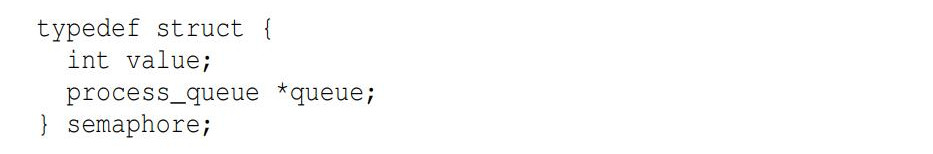
\includegraphics{10.6_1.jpg}}
    \scalebox{2}{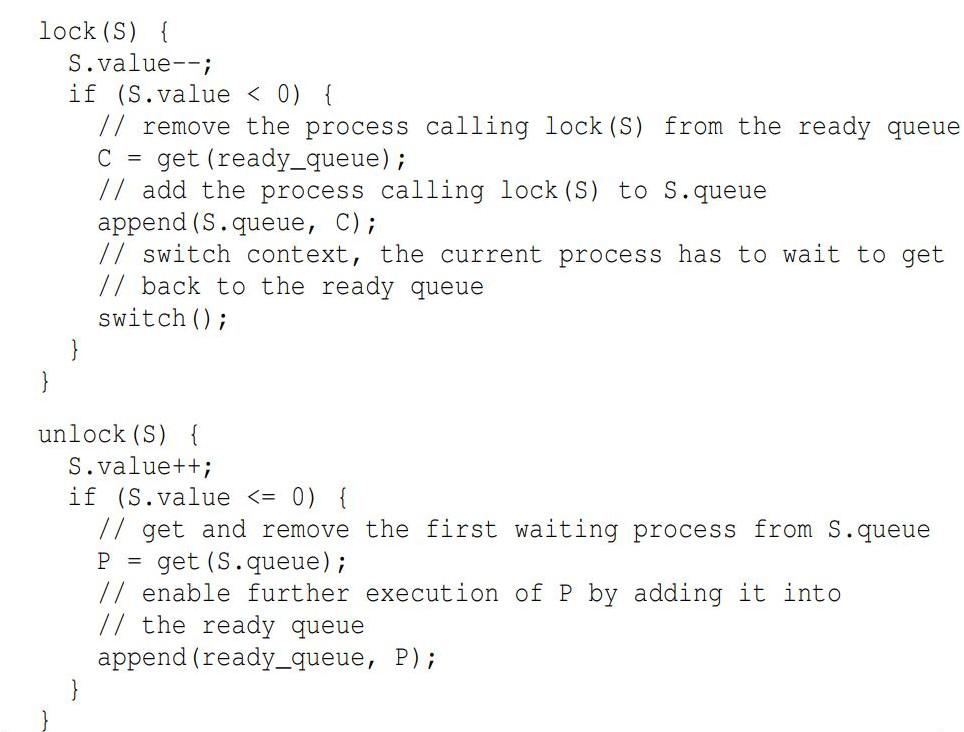
\includegraphics{10.6_2.jpg}}
    \caption{prevzat z prezentace IOS: Synchronizace procesu - kod implementace semaforu}
\end{figure}

\newpage
\section{}
\textbf{Jedenacta prednaska:} Pokracovani a dokonceni synchronizace procesu, monitory, deadlock

\subsection{Monitory}
Synchronizacni prostredky (jeste) vyssi urovne (nez semafory). Problem semaforu v realnem kodu je, ze \textbf{je zde spousta sdilenych dat, ktere se budou vzajemne vylucovat} - nechceme mit cely program zamkly - bude zde snaha zamknuti minimalizovat - muze se stat, ze se nekde v nejake vetvi \textbf{zapomene lock/unlock a nastane problem} (v realnem kodu tak semafory jednoduche nejsou).

Proto vznikl komfortnejsi synchronizacni mechanismus - monitory. V systakticke podobe vypadaji takto (jazyk Ada, bezne se takto nepouzivaji):

\begin{figure} [h]
    \centering
    \scalebox{2}{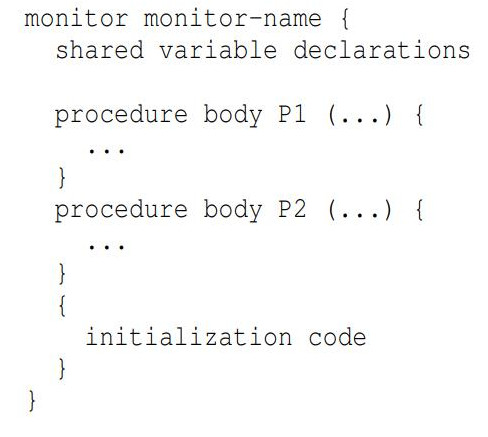
\includegraphics{11.1_1.jpg}}
    \caption{z prezentace IOS: Synchronizace procesu - kod monitoru}
\end{figure}

\textbf{Monitor:}
\begin{itemize}
    \item je mozne si predstavit jako datovou strukturu podobne tride se sdilenymi promennymi,
    \item ty jsou sdileny ruznymi procesy pracujici s monitorem,
    \item procesy se mohou k promennym dostat pres procedury (metody monitoru),
    \item automaticky monitor zajistuje, ze v danem okamziku pobezi na nem nejvyse 1 metoda,
    \item kdokoli chce pracovat se sdilenymi zdroji, musi pouzivat tyto metody a zde se automaticky zajisti zamek/odemknuti zdroju,
    \item pouziti - do monitoru se nadefinuji sdilene zdroje, dale mechanismy, jak se k nim ma pracovat (procedury), dale konstruktor (inicializacni kod) \\
\end{itemize}

\newpage

\textbf{Popis monitoru:}
\begin{itemize}
    \item slupka (okraje) predstavuji ochrannou barieru monitoru,
    \item do monitoru je mozne vstoupit definovanymi operacemi  (dvere),
    \item pokazde kdyz do monitoru nekdo vstoupi, tak se dvere uzamcou.
    \item dalsi "zajemci" o vstup jsou zarazeni do cekaci fronty vne monitoru (zarazovani tim, ze volaji dane operace v okamziku zamknuteho monitoru),
    \item pokud se chteji synchronizovat, pouziji bud preddefinovane podminky programatorem, s kazdou z tech podminek se poji dalsi cekaci fronta (chci se sync pomoci podminky x - wait\_x() - zarazeni do fronty x - soucasne bude vybran nekdo, kdo ceka na vstup monitoru a bude moznost v nem bezet - ja cekam ve fronte x na nekoho, kdo se do monitoru dostane a provede signal ci notify - muze me uvolnit z fronty x) \\
\end{itemize}

\begin{figure} [h]
    \centering
    \scalebox{2}{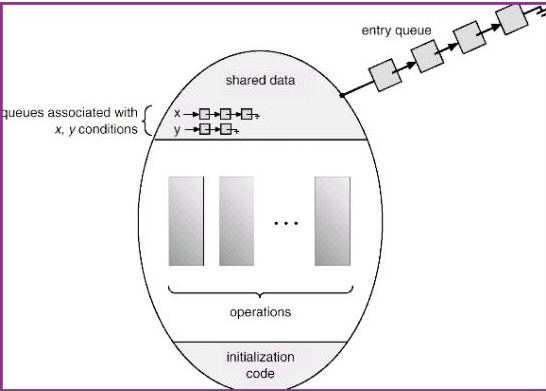
\includegraphics{11.1_2.jpg}}
    \caption{z prezentace IOS: Synchronizace procesu - graficke ztvarneni monitoru}
\end{figure}

\textbf{Co kdyz se procesy chteji synchronizovat uvnitr monitoru?}
\begin{itemize}
    \item pouzivaji se mechanismus podminek - conditions,
    \item specialni datova struktura, s definovanymi operacemi nad ni, pomoci nich se procesy synchronizuji,
    \item je mozne volat wait() - synchronizovat se s nekym na nejake podmince,
    \item je mozne nekomu kdo na podmince ceka poslat uvolnujici signal (operace signal() nebo notify())
\end{itemize}

\textbf{Rozliseni signal a notify:}
\begin{itemize}
    \item v monitoru muze bezet jen jeden proces,
    \item pokud v nem jsou dva (z toho jeden ve fronte dane podminky [napr. proces ve fronte x, druhy v monitoru a vola signal/notify]
    \item signal() - po zavolani pokracuje ten, kdo signal dostane (ten kdo je ve fronte [x]) a bezi v monitoru, druhy proces se zaradi bud do cekaci fronty ci se zaradi do dalsi fronty uvnitr monitoru, kde takoveto procesy cekaji (a maji prednost pred procesy ve fronte venku)
    \item notify() - po zavolani pokracuje volajici, resp ten kdo signal dostal (ten co byl ve fronte se presune bud do fronty mimo monitor ci do jine fronty uvolnenych procesu ale cekajicich)
    \item ceka se, az bude proces odejde z monitoru nebo zacne cekat (zaradi se do fronty podminky)
    \item pokud nikdo na podmince neceka a nekdo na ni pouzije signal ci notify, jedna se o prazdnou operaci (nic se neprovede) \\
\end{itemize}

Monitory je mozne implementovat \textbf{s vyuzitim semaforu} (vstupni semafory, semafory ke kazde podmince, pro prioritni procesy - pozastavene procesy ve fronte uvnitr monitoru). Monitory jsou dostupne v Jave ci C\#. V POSIXu (C, C++, ..), jsou k dispozici alespon podminky (kombinace semaforu a podminek) - pthread\_cont\_t a funkce pthread\_cond\_wait / signal / broadcast. \\

\newpage

\subsection{(Nektere) Klasicke synchronizacni problemy}
\subsubsection{Problem producenta a konzumenta}
\begin{itemize}
    \item mame smecku procesu, predem rozdeleny, ci se dynamicky deli na producenty a konzumenty, komunikuji spolu pres vyrovnavaci pamet (napr. pole s kruhovym bufferem),
    \item nutne procesy synchronizovat pro spravnou praci s pameti,
    \item resenim jsou tri semafory (full, empty, mutex),
    \item full - rika kolik polozek je aktualne v cache k dispozici, zamykanim si rezervuji polozku v pameti ke spotrebe,
    \item empty - rika kolik je volnych slotu v cache, zamykanim se rezervuje kapacita pro zapis do cache,
    \item mutex - pomocny semafor, ktery se zamkne pri praci s ukazovatky do cache,
    \item \textbf{semafory je nutne vhodne inicializovat} (full=0, empty=max. hodnota cache, mutex=1) \\
\end{itemize}

\begin{figure} [h]
    \centering
    \scalebox{2}{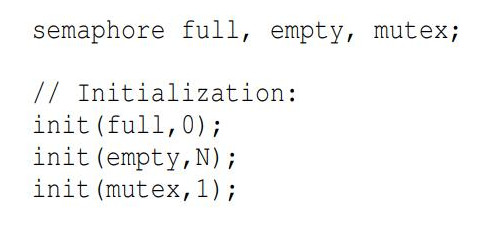
\includegraphics{11.2.1_1.jpg}}
    \caption{z prezentace IOS: Synchronizace procesu - sync prostredky producentu a konzumentu}
\end{figure}

\newpage

\textbf{Pseudokod producenta:}
\begin{itemize}
    \item pracuji tak, ze vyprodukuji polozku, kterou chteji zapsat do cache,
    \item nejprve zamknou empty (pokud se to podari - je tam volne misto a rezervuji si ho pro sebe),
    \item zamknou mutex,
    \item zacnou zapisovat do cache (posunou ukazovatko),
    \item odemkne se pristup do cache - odemknuti mutex a full (konzumentum se da najevo, ze je zde polozka ke konzumaci),
    \item pracuje v nekonecnem cyklu do while 1 \\
\end{itemize}

\textbf{Pseudokod konzumenta:}
\begin{itemize}
    \item nejprve zamknou full (pri uspechu - ve vyrovnavaci pameti je neco ke konzumaci, polozku si alokovali),
    \item zamknou si pristup k cache (zamkne se mutex),
    \item z vyrovnavaci pameti se odstrani 1 polozka,
    \item odemkne se pristup k cache (mutex) a nasledne se odemkne empty (da se najevo producentum, ze se v cache uvolnila polozka),
    \item zkonzumuje se polozka,
    \item pracuje v nekonecnem cykly do while 1 \\
\end{itemize}

\begin{figure} [h]
    \centering
    \scalebox{2}{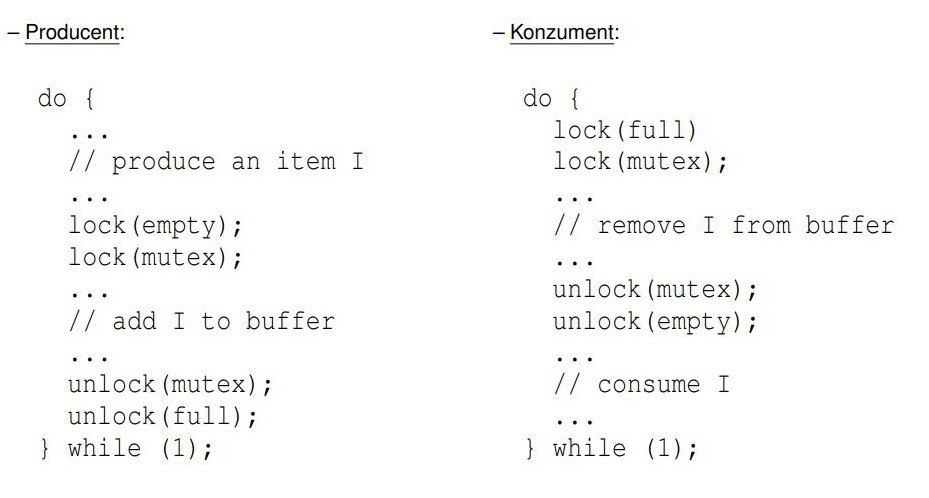
\includegraphics{11.2.1_2.jpg}}
    \caption{z prezentace IOS: Synchronizace procesu - pseudokod producenta a konzumenta}
\end{figure}

\newpage

\subsubsection{Problem ctenaru a pisaru}
\begin{itemize}
    \item dva typy procesu - ctenari a pisari,
    \item pracuji se sdilenou pameti - ctenari ji mohou pouze cist, pisari jen menit,
    \item muze soucasne cist libovolny pocet ctenaru (nemeni se obsah pameti),
    \item pokud nejaky pisar, nesmi nikdo ani cist, ani psat,
    \item pouzva se sdilena promenna readcount - pocet ctenaru,
    \item nutne pouzit semafor mutex (chranici pristup k readcout) a semafor wrt (semafor pisaru),
    \item opet je nutna inicializace (pocet ctenaru=0, oba semafory=1) \\
\end{itemize}

\begin{figure} [ht]
    \centering
    \scalebox{2}{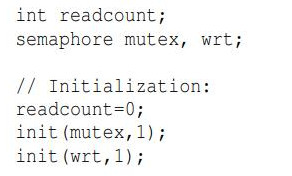
\includegraphics{11.2.2_1.jpg}}
    \caption{z prezentace IOS: Synchronizace procesu - sync prostredky ctenaru a pisaru}
\end{figure}

\textbf{Pseudokod pisare:}
\begin{itemize}
    \item pokud chce zapisovat zamkne semafor wrt,
    \item az se mu to poradi, zapisuje,
    \item po dopsani odemkne wrt,
    \item pracuje v do while 1 cyklu \\
\end{itemize}

\textbf{Pseudokod ctenare:}
\begin{itemize}
    \item v okamziku kdyz chce cist,
    \item je nutne zamknout pristup k promenne readcount (mutex), pote ji inkrementovat (zjisti tak, jestli je prvni),
    \item pokud readcout==1, tak se jedna o prvniho ctenare,
    \item potom se zamkne wrt a odemkne se mutex (readcount),
    \item zacne cist (pokud prijde dalsi ctenar, pouze readcount inkrementuje a cte),
    \item jakmile ctenar docte, zamkne mutex,
    \item dekrementuje se readcount, pokd je ==0, znamena to, ze je poslednim ctenarem a musi odemknout pristup pisarum (wrt),
    \item odemkne se pristup k readcount (mutex),
    \item pracuje v do while 1 cyklu \\
\end{itemize}

\begin{figure} [ht]
    \centering
    \scalebox{2}{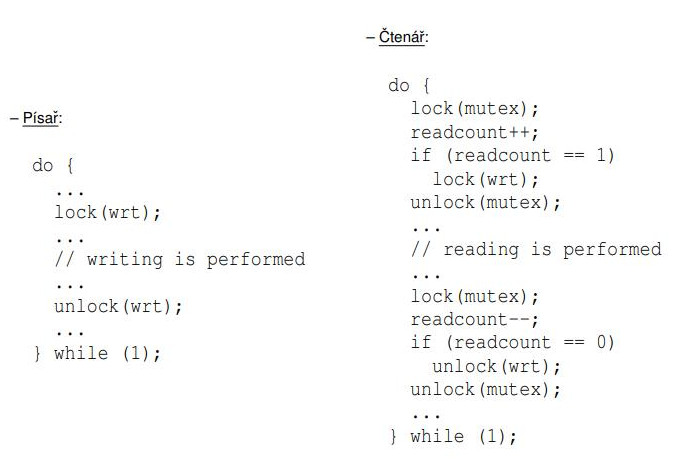
\includegraphics{11.2.2_2.jpg}}
    \caption{z prezentace IOS: Synchronizace procesu - pseudokod ctenaru a pisaru}
\end{figure}

Toto reseni ma nevyhodu - \textbf{hrozi vyhladoveni pisaru} - pokud do kriticke sekce vejde 1 ctenar, prijde pisar a zacne cekat, prijde dalsi ctenare, vejde do kriticke sekce, prvni odejde, druhy taky, ale opet vejde prvni ctenar - do nekonecna se tu stridaji a pisar nikdy nezapise. Vyhladoveni je nekdy tolerovano, ale je dobre se mu vyhnout (mala pravdepodobnost, ze ctenari se budou do nekonecna stridat).

\textbf{Reseni vyhladoveni:}
\begin{itemize}
    \item pouzije se dalsi semafor - wrt\_waiting - cekajici pisar,
    \item pisar nejprve zamkne wrt\_waiting, pote wrt, po zamknuti wrt odemkne wrt\_waiting,
    \item ctenari na zacatku provedou lock wrt\_waiting, unlock wrt\_waiting a pote pokracuji dal (zajisti, ze pokud nejaky pisar zacne cekat, tak vsichni ctenari doctou, a po navratu na zacatek nebudou schopni provest lock unlock) \\
\end{itemize}

\newpage

\subsubsection{Problem vecericich filozofu}
\begin{itemize}
    \item 5 filozofu, kteri reprezentuji procesy,
    \item sesednou se kolem kulateho stolu, kteri budou jist a debatovat, jedi pomoci asijskych hulek, ktere budou mit rozdeleny tak, ze mezi kazdymi filosofy je jedna hulka (ji se dvema..) - 5 hulek pro 5 filozoru,
    \item cyklus: ziska si svoji levou a pravou hulku, muze se najist, polozi hulky zpet, premysli, pote opet ji,
    \item reprezentuje situaci, kdy mezi synchronizovanymi procesy je cyklicka zavislost \\
\end{itemize}

\textbf{Moznost reseni:}
\begin{itemize}
    \item ne dokonale reseni, moznost uvaznuti (=spatne) a
    \item je mozne, ze dva filosofove budou jist soucasne 1 hulkou,
    \item zavede se 5 binarnich semaforu (pole semaforu),
    \item vsechny inicializovane tak, ze jsou odemknute \\
\end{itemize}

\textbf{Filozof I:}
\begin{itemize}
    \item i = ID, hodnota 0-4,
    \item zamkne hulku i, nasledne zamkne hulku i+1 modulo 5,
    \item pokud se podari zamek obou hulek, naji se,
    \item nasledne odemkne obe hulky,
    \item muze premyslet,
    \item do while 1 cyklus \\
\end{itemize}

\begin{figure} [htb]
    \centering
    \scalebox{1.6}{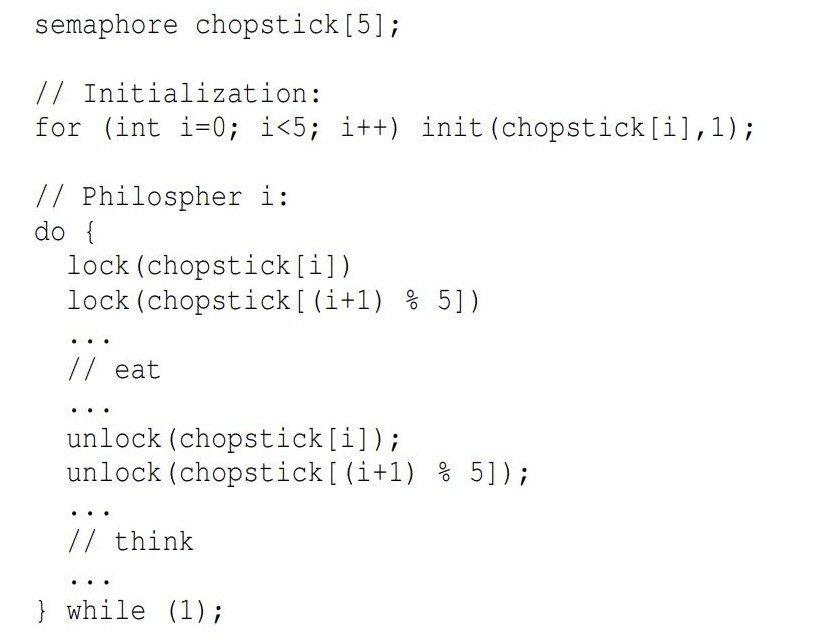
\includegraphics{11.2.3.jpg}}
    \caption{z prezentace IOS: Synchronizace procesu - pseudokod reseni tohoto problemu}
\end{figure}

\newpage

\textbf{Gde deadlock?}
\begin{itemize}
    \item procesy za planovani se mohou naskladat tak,
    \item ze kazdy si vezmne svoji svoji levou hulku (kazdy hulku se stejnym cislem jako jeho cislo 4-4, 0-0),
    \item nasledne si kazdy z nich bude chtit ziskat tu druhou,
    \item bude kazdy trvat na tom, ze si svoji necha a chce tu druhou,
    \item cely system se zastavi - deadlock \\
\end{itemize}

\textbf{Reseni deadlocku zde:}
\begin{itemize}
    \item jednou z moznosti je ziskavat obe hulky soucasne,
    \item napr. pomoci semaforu system 5, umoznuji zamknout pole semaforu,
    \item dalsi moznosti je ziskavat hulky asymetricky - alespon 1 z filozofu bude brat hulky v obracenem poradi (napr. kazdy lichy filozof bude brat hulky nejprve i a pote i+1 modulo 5 a sudi nejprve i+1 modulo 5 a potom i) \\
\end{itemize}

\newpage

\subsection{Deadlock (uvaznuti)}
\subsubsection{Definice}
\textbf{\textit{Uvaznutim (deadlockem) pri pristupu ke zdrojum s vylucnym (omezenym) pristupem rozumime situaci, kdy kazdy proces z nejake neprazdne mnoziny procesu je pozastaven a ceka na uvolneni nejakeho zdroje s vylucnym (omezenym) pristupem vlastneneho nejakym procesem z dane mnoziny, ktery jediny muze tento zdroj uvolnit, a to az po dokonceni jeho pouziti.}} \\

\textbf{Vysvetleni definice:}
\begin{itemize}
    \item je specialni pripad deadlocku,
    \item neprazdna mnozina procesu = 1, 2, 1000, ... ne 0! - pouzivame tuto definici, jine pouzivaji mnozinu procesu kde je jich alespon 2,
    \item vylucny pristup = zdroj, ktery pouziva v danem okamziku nanejvys 1 proces,
    \item omezeny pristup = zobecnene kriticke sekce, kde zdroj muze pouzivat urcity pocet procesu, ale ne neomezeny pocet,
    \item pozastaven = neni tam aktivni cekani, nebezi (pokud to tam nebude, nebylo by mozne rozlisit deadlock a livelock),
    \item zdroj vlastneny nejakym procesem z dane mnoziny = obvykle jiny, muze to byt i stejny proces,
    \item jediny ... po dokonceni jeho pouziti = pracujeme s tim, ze se pouziva zamek, ktery se pouziva neomezene (zadny casovy zamek), nikdo nemuze zdroj vzit, odemknout, nikde neni zadny casovac,
    \item kardinalita-pocet procesu mnoziny procesu=1 - tzv. self deadlock - proces zamkne zdroj a pak ho pokusi zamknout jeste jednou (doublelocking) \\
\end{itemize}

\textbf{Obecnejsi definice:} (s moznosti uvaznuti i bez prostredku s vylucnym pristupem - napr. zasilani zprav): \\
Uvaznutim rozumime situaci, kdy kazdy proces z nejake neprazdne mnoziny procesu je pozastaven a ceka na nejakou udalost, ktera by mohla nastat pouze tehdy, pokud by mohl pokracovat nektery z procesu z dane mnoziny. (je to napr. situace kdy proces 1 ceka na zpravu od procesu 2, ten ceka na zpravu od 3, 3 ceka na 4, ... proces 5 ceka na zpravu od 1 - obecnejsi uvaznuti)


\subsubsection{Typicky priklad deadlocku}
\begin{itemize}
    \item pri pristupu ke zdrojum s vylucnym omezenym pristupem,
    \item v praxi mohou byt jednotliva volani ve zdrojaku velmi daleko od sebe a zamykany mohou byt jen za urcitych podminek,
    \item uvaznuti se tak projevi jen zridka a spatne se odaluje \\
\end{itemize}

\newpage

\begin{figure} [htb]
    \centering
    \scalebox{2}{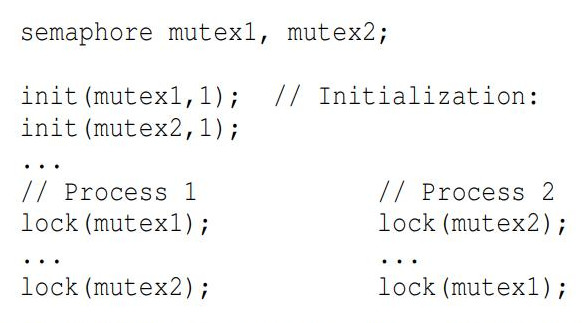
\includegraphics{11.3.jpg}}
    \caption{z prezentace IOS: Synchronizace procesu - priklad uvaznuti}
\end{figure}

\textbf{Popis (kodu):}
\begin{itemize}
    \item dva semafory, oba na zacatku odemknute,
    \item za predpokladu pouziti standardnich semaforu se standardni semantikou, neni zde jadro, ktere napr. hlida situaci a jeden z procesu by zabilo, ..
    \item jeden proces zamkne prvni mutex, neco provede, pokusi se zamknout druhy,
    \item druhy proces zamkne druhy mutex, neco provede a zamkne prvni,
    \item nastane deadlock \\
\end{itemize}

\subsubsection{Coffmanovy podminky}
Rozvadi to, co je obsahem uvaznuti do 4 nutnych a postacujicich podminek, ktere jsou zapotrebi pro uvaznuti. 

\textbf{K tomu aby uvaznuti mohlo nastat je nutne ci postacuji nasledujici podminky:}
\begin{itemize}
    \item vzajemne vylouceni pri pouzivani prostredku,
    \item vlastnictvi alespon 1 zdroje, pozastaveni a cekani na dalsi,
    \item prostredky vraci (pouze) ten proces, ktery jej vlastni a to po dokonceni jejich vyuziti (zdroj je vlastnen procesem, pouze ten proces ho muze vratit a to po dokonceni vyuziti toho zdroje),
    \item cyklicka zavislost na sebe (navzajem) cekajicich procesu (rozumi se tim to, ze jeden proces ceka na druheho - zadne aktivni cekani v cyklu) \\
\end{itemize}

\subsubsection{Reseni uvaznuti}
\begin{itemize}
    \item prevence uvaznuti,
    \item vyhybani se uvaznuti,
    \item detekce a zotaveni \\
\end{itemize}

Zakladni spolecna myslenka vsech reseni je \textbf{princip, kterym se snazi zrusit platnost alespon jedne z nutnych podminek k uvaznuti} (Coffmanovych podminek - kdyz se jedna zneplatni - nemuze dojit k uvaznuti). \\

\subsubsection{Prevence uvaznuti}
\textbf{Resi, jak tyto podminky zneplatnit:}
\begin{itemize}
    \item prvni (vylouceni)
    \begin{itemize}
        \item nepouzivat zadne sdilene prostredky nebo uzivat sdilene prostredky,
        \item ale pouze takove, ktere umoznuji skutecne soucasny sdileny pristup
        \item a u kterych neni nutne vzajemne vylouceni procesu (ne vzdy problem pujde vyresit timto zpusobem),
    \end{itemize}
    \item druha (vlastnictvi)
    \begin{itemize}
        \item proces muze zadat o prostredky pouze tehdy, pokud zadne nevlastni,
        \item (kdyz chce proces pouzivat soucasne 5 zdroju v jednom okamziku, musi zamknout vsechny soucasne - ziska nebo ceka - systematicky v kodu zamkykam vsechny nebo zadny zdroj - kontrola zamku: pokud proces jiz neco zamkl, nemuze znovu zamykat - musi vse uvolnit a pote muze zamknout),
        \item nevyhodou je nutnost zamknuti vsech zdroju, ktere se pouzivaji soucasne (napr. 30 min se pouziva 1 zdroj, pote 1 min se pouziva dalsi zdroj soucasne s prvnim - musi se zamknout na 30 min oba zdroje),
    \end{itemize}
    \item treti (navrat)
    \begin{itemize}
        \item nebudu vyzadovat, aby proces vzdy ziskal vsechny zdroje, ktere chce pouzivat soucasne v 1 okamzik,
        \item ale umoznim mu ziskavat postupne dalsi a dalsi zdroje, postupne prizamykat tyto zdoje,
        \item ale jen v situaci, kdy je opravdu mozne tyto zdroje ziskat,
        \item pokud se proces pokusi neco prizamknout a ono se to nepovede, bude to reseno specialnim zpusobem
        \item (napr. tak, ze proces bude zabit a vsechny zdroje mu budou odebrany),
        \item nevyhodou je situace, kdy v okamziku kdy se proces zabije, uz mohl s nekterymi zdroji neco delat, zdroje mohou byt v nekonzistentnim stavu (idealne se pokust vratit zdroje do konzistentniho stavu),
    \end{itemize}
    \item ctvrta (cyklicka zavislost)
    \begin{itemize}
        \item zavedenim usporadanim nad zdroji (ocislovani),
        \item je mozne tyto zdroje ziskavat pouze od urciteho poradi (napr. od nejmensiho k nejvetsimu - zacnu 1, pak 2, pak 3, .. - pokud zamknu 5, muzu zamknout 5+, ale 3 uz ne), 
        \item bud se konstrukci programu zajisti, aby se vzdy zamykalo v tomto poradi, a pote analyzou, auditem se overi, zda opravdu ma program takovou zamykaci disciplinu,
        \item anebo budu mit system zamykani, ktery toto bude kontrolovat \\
    \end{itemize}
\end{itemize}

Ke vsem bodum se da rict, ze bud bude program navrhovan tak, aby byl konformni s pouzitou strategii nebo se vynuceni stragie kontrolovat az pri behu. \\

\subsubsection{Vyhybani se uvaznuti}
Dalo by se to se chapat jako prevence 4. Coffmanovy podminky. \textbf{Obecny princip:}
\begin{itemize}
    \item procesy musi predem deklarovat (jadru, systemu zpravy zdroju) informace o tom, jake zdroje a jak budou pouzivat, resp. ktere zdroje se budou pouzivat a kolik jednotek zdroje se bude pouzivat - nejjedoduseji musi kazdy proces rict, kolik jednotek ktereho zdroje bude pouzivat (dalsi informace napr. budu pouzivat zdroje 1 2 3 4, nikdy nebudu pouzivat soucasne 1 a 2, apod.),
    \item nasledne system pridelovani zdroju si vede informace co ty procesy deklarovaly,
    \item o jejich moznych pozadavcich,
    \item soucasne si vede o aktualnim stavu pridelovani (vi kdo co vlastni a kdo o co pozadal),
    \item v okamziku kdy system ma neuspokojene zadosti, ty uspokoji tehdy, pokud nemuze vzniknout zadna cyklicka zavislost na sebe cekajicich procesu, ani v tom nejhorsim moznem pripadu, ktery by mohl nastat s ohledem na to, co procesy deklarovaly \\
\end{itemize}

\textbf{Priklad:}
\begin{itemize}
    \item situace v bance,
    \item od klientu mam sverene penize na terminovane vklady, vim kdy si klienti mohou sve vklady vybrat,
    \item prijde nekdo a bude chtit pujcku,
    \item je nutne se zamyslet kolik zdroju mam a kdy si to klienti mohou vybrat,
    \item pujcu mohu dat jen tehdy, kdyz v nejhorsim moznem pripade (vsichni klienti si pujdou vybrat co mohou) se nedostanu do dluhu,
    \item mohu penize pujcit \\
\end{itemize}

\textbf{Algoritmus zalozeny na grafu alokace zdroju:}
\begin{itemize}
    \item resi problem vyhybani se uvaznuti,
    \item pro pripad binarnich zdroju,
    \item je veden systemem, ktery zdroje prideluje, ten si prubezne udrzuje graf vztahu mezi procesy a zdroji - dva typy uzlu (procesy a zdroje) a tri typy hran - hrany od zdroje k procesu (ktery zdroj je kym vlastnen, zvyraznena, "tucna" hrana), hrany Pi a Ri od procesu ke zdroji (kdo o ktery proces zada), Pi a Ri od procesu ke zdroji (kdo o ktery zdroj muze pozadat - zvyraznena hrana, "tucna")
    \item zdroj system pridely pouze tehdy, pokud posoudi, ze v budoucnu nemuze nastat cyklicka zavislost procesu, jednoduse tim, ze "cvicne" provede otoceni zadosti na hranu vlastnictvi (z P2 do R2 udela R2 do P2), pokud v te situaci vznikne v grafu cyklus, znamena to, ze v budoucnu by mohl vzniknout deadlock,
    \item v takovem okamziku system nepovoli prideleni zdroje (proces bude muset dal cekal na uvolneni zdroje, i kdyz je volny) \\
\end{itemize}

Pokud by se pouzivaly obecne zdroje se zobecnenou kapacitou, pouzil by se tzv. bankeruv algoritmus. \\

\subsubsection{Detecke uvaznuti a zotaveni}
System pridelovani zdroji \textbf{umozni pripadny vznik uvaznuti} (pokud pomineme to, ze externe k mnozine uvaznutych procesu mame "strazneho andela", ktery uvaznuti vyresi), \textbf{ale periodicky} (bezi specialni proces, zajistujici ze nebude prebit prioritami jinych procesu) \textbf{se detekuje, jestli k uvaznuti nedoslo}, a pokud ano, provede se zotaveni.

\textbf{Detekce uvaznuti:}
\begin{itemize}
    \item vedeni grafu vlastnictvi zdroju a cekani na zdroje (obdobny jak u vyhybani se uvaznuti) - stejny pocet uzlu, 2 typy hran (nekdo zada o zdroj, nekdo vlastni zdroj),
    \item pokud vznikne v grafu cyklus, vim, ze uvaznuti nastalo \\
\end{itemize}

\textbf{Zotaveni z uvaznuti:}
\begin{itemize}
    \item alespon nekterym procesum, ktere uvazly, odeberu zdroje,
    \item proces se bud zrusi pozastavi se s tim, ze muze pokracovat, az bude moci ziskat vsechny zdroje, ktere potrebuje,
    \item muze nastat problem - procesy zabiju, mohou mit ve zdrojich rozpracovane nejake operace - zdroje mohou byt v nekonzistentnim stavu - nutnost but nechat system uvaznuty, nebo se spokojit s nekonzistencemi, nebo system navrhnout tak, ze pri zabiti procesu se nezabije ihned, ale prvne provede zotaveni (rollback - anuluje sve operace a dostane zdroje do konzistentniho stavu) \\
\end{itemize}

\newpage

\subsection{Formalni verifikace, verifikace s formalnimi koreny}
Moznosti odhalovani nezadouciho chovani ystemu (uvaznuti, starnuti):
\begin{itemize}
    \item inspekce systemu - nez se kod nasadi, krome vyvojare kod musi projit i nekdo dalsi (ci skupina), kteri schvali, ze kod pochopili a je podle nich bezchybny,
    \item simulace, testovani - vestavene systemy -  vytvori si model systemu a z nej se generuje kod, na modelu overuji chovani systemu - nevyhodou testovani na jedne jednotce (modelu) je to, ze se chyba nemusi projevit (nedeterminismus se nemusi projevit) - paralelni programy - vkladani sumu do planovani (na kriticka mista pred ne se vlozi nahodne zpozdeni, prepnuti kontextu), zvysi se tim mnozstvi prolozenych aktivit a sance ze se najde chyba,
    \item dynamicka analyza - sleduje se co se deje v systemu, pote je snaha extrapolovat (="vestit"), co by se mohlo stat,
    \item formalni verifikace ci verifikace s formalnimi koreny - pokud se rekne, ze program nema chybu ci urcitou vlastnost, tak ji ma s platnosti matematickeho dukazu,
    \item nebo kombinace vyse uvedenych pristupu \\
\end{itemize}

Experimentuje se i s automatickymi opravami - je zde \textbf{behovy system, ktery monitoruje, co se deje}, pokud uvidi, ze nastala chyba, \textbf{pokusi se ji opravit automaticky} (napr. sledovani date race conditions - pri poruseni vzajemneho vylouceni pri pristupu ke sdilene promenne se automaticky prida zamek - mohu ale tzv. pacienta zabit - zpusobit uvaznuti, proto se napriklad misto toho pred praci s danou promennou misto vkladani zamku vynuti prepnuti kontextu - zvysi se sance, ze se projde kritickou sekci bez prepnuti kontextu)

\textbf{Proces formalni verifikace:}
\begin{itemize}
    \item vytvoreni modelu - vytvori se zdrojovy kod, ci model, ktery se bude verifikovat (ci kombinaci, napr. cast jadra OS a model OS, odlehcenou implementaci),
    \item specifikace vlastnosti, ktere maji byt overeny - mohou to byt genericke vlastnosti napr. v systemu nesmi byt deadlock nebo slozitejsi vlastnosti napr. v cache neni nikdy vice nez 10 polozek,
    \item kontrola (automaticka), zda model splnuje specifikaci \\
\end{itemize}

\textbf{Overovani se provadi metodami:}
\begin{itemize}
    \item model checking (kontrola modelu),
    \item theorem proving (dokazovani teoremu),
    \item static analysis (staticka analyza) \\
\end{itemize}

Nad ramec verifikace se take provadi automaticka analyza dle dane specifikace - doda se specifikace, jake vlastnosti system ma byt, pro urcite tridy systemu je mozne automaticky vysyntetizovat korektni implemetaci.

\newpage

\subsubsection{Theorem proving}
\begin{itemize}
    \item teoremem je zde veta, ktera rika 'Muj program XXX spluje XXX specifikaci',
    \item pouzivaji se poloautomaticke dokazovaci prostrek (eviduji, co uz jste dokazali, maji db standardne platnych skutecnosti z logiky, znaji pravidla spravneho odvozovani),
    \item vyzaduje se expert, ktery urcuje, jak se dukaz ma vest (presto se to pouziva, napr. Mikrojadra ProvenCore ci seL4),
    \item existuji i plne automaticke dokazovace (rozhodovaci procedury, umi automaticky rict zda plati ci ne) - obvykle pro omezene fragmenty logik, spise se pouzivaji jako pomocne \\
\end{itemize}

\subsubsection{Model checking}
\begin{itemize}
    \item obvykle plne automatizovany pristup, prostredek,
    \item zalozen na systematickem generovani stavu systemu a stavoveho prostoru (systematicky se hleda, zda nekde neni chyba),
    \item nevyhodou je obrovsky pocet stavu - napr. pri N dvoustavovych procesech (procesy zacnou a skonci), muze se vygenerovat $2^N$ stavu - problem stavove exploze \\
\end{itemize}

\subsubsection{Static analysis}
\begin{itemize}
    \item snaha analyzy a verifikace systemu na zaklade jeho zdrojoveho kodu, aniz by se tento kod provadel (nebo alespon ne v puvodni semantice - napr. celociselne promenne 0 - 1235, pamatuji si jen jestli je hodnota zaporna, 0 ci kladna),
    \item nejjednodusi staticky analyzator je grep (naji se syntakticke vzory chyb a grepem se vyhledavaji),
    \item ma ruzne podoby: data flow analysis, constraint analysis, type analysis, abstract interpretation, symbolic execution, ..
    \item nastroje: Facebook Infer, Frama-C, Microsoft SDV, SpotBugs, cppcheck, ... \\
\end{itemize}

\newpage

\section{}
\textbf{Dvanacta prednaska:} Zacatek spravy pameti.
\subsection{Sprava pameti}
Aby program mohl byt proveden, musi byt spusten - musi byt nad nim vytvoren proces, msui mu byt pridelen procesor a take pamet (a dalsi zdroje - soubory, ..) \\

\textbf{Rozlisujeme:}
\begin{itemize}
    \item logicky adresovy prostor - LAP - je virtualne adresovy prostor, se kterym pracuje CPU pri provadeni kodu (uzivatelskeho ci jadra - kazdy proces i jadro maji sve logicke adresove prostory),
    \item fyzicky adresovy prostor - FAP - adresovy prostor fyzickych adres pameti (obsahuje adresy, ktere se umistuji na adresove sbernici, chcemeli z pameti nacist nebo do ni zapsat - je spolecny pro vsechny procesy i jadro) \\
\end{itemize}

Casto logicky adresovy prostor \textbf{jadra byva podprostorem logickeho adresoveho prostoru jednotlivych procesu}. Vsechny logicke adresove prostory procesu (v Linuxu) se prekryvaji ve stejne casti - \textbf{v casti, kde je LAP jadra}. LAP jadra \textbf{neni} ale procesum pristupny. Vyhodou je, ze pri prechodu rezimu procesu na rezim jadra se \textbf{pouze zpristupni tento LAP} nebo pri prepinani procesu (krome zmen mapovani casti LAP procesu) se \textbf{nemusi menit mapovani pro cast LAP jadra}.

\textbf{Proces pracuje s logickymi adresami, ale na adresovou sbernici se umistuji fyzicke adresy}. Toto mapovani provadi \textbf{MMU (Memory Management Unit):}
\begin{itemize}
    \item HW jednotka specializovana na predklad logickych adres na fyzicke, 
    \item dnes bezne soucasti cipu CPU,
    \item provadi preklad na zaklade datovych struktur,
    \item obsah struktur je castecne ulozen ve specialnich registrech, castecne v hlavni pameti systemu,
    \item soucasti MMU je cache, obvykle TLB, pro urychleni prekladu \\
\end{itemize}

\textbf{Komunikace CPU a pameti:}
\begin{itemize}
    \item na CPU bezi programy (CPU pracuje s logickymi adresami),
    \item pri cteni/zapisu logicke adresy,
    \item adresa se preda do MMU,
    \item MMU provede preklad logicke adresy na fyzickou,
    \item MMU umisti fyzickou adresu sbernici a po ni se prenesou data/kod mezi pameti a CPU \\
\end{itemize}

\newpage

\subsection{Pridelovani pameti}
Existuje vice urovni pridelovani pameti. V \textbf{nejnizsich (z hlediska blizkosti hw) se prideluje FAP pro zamapovani do LAP}, pote jsou napr. pridelovani pameti pres knihovni funkce (malloc - mimo rezim jadra ci kmalloc, vmalloc - jadro), az po vyseurovnove pridelovani v ramci aplikaci. 

Nejnizsi uroven pridelovani je \textbf{implementovana v jadre a jedna se o pridelovani FAP pro zamapovani LAP}. Bezne zpusoby pridelovani pameti (a mapovani LAP na FAP):
\begin{itemize}
    \item pridelovani po spojitych blocich (contiguous memory allocation),
    \item segmentech,
    \item strankach,
    \item kombinace vyse uvedeneho (intel - segmenty a stranky) \\
\end{itemize}

\textbf{Funkce malloc:}
\begin{itemize}
    \item pri zadosti o alokaci nejakeho kusu pameti (poctu bajtu),
    \item musi malloc pozadat jadro o prideleni FAP,
    \item pozaduje od jadra vetsi blok pameti (segment, stranka),
    \item z bloku pameti se vykousne pozadovany pocet bajtu,
    \item ty dostane k dispozici uzivatel,
    \item pri volani dalsich mallocu, dokud pozadovany pocet bajtu nebude vetsi nez prideleny blok, nepujdou pozadavky do jadra, ale bude se cerpat jiz prideleny prostor \\
\end{itemize}

\subsection{Contiguous Memory Allocation}
Mechanismus mapovani logickych adres na fyzicke a pridelovani pameti po spojitych blocich. Jedna se o \textbf{nejjednodusi mechanimus z hlediska hw, tak obsluhy OS}. V beznych vypocetnich systemech se prilis \textbf{nepouziva}, nicmene je vhodny pro jednoduche a vestavene aplikace, ktere maji bezet na jednoduchem hw.

\textbf{Popis:}
\begin{itemize}
    \item je to po spojitych blocich (neco jako ukladani dat spojite),
    \item k popisu takoveho mapovani je treba znat, ve kterem FAP je zamapovan pocatek LAP,
    \item je nutne vedet, jak je usek pameti velky (pro odchyceni pristupu mimo meze tohoto prostoru) \\
\end{itemize}

\textbf{Preklad adresy:}
\begin{itemize}
    \item MMU si pro aktualne bezici proces pamatuje 2 udaje,
    \item v limitnim registru si pamatuje, kolik proces pameti dostal,
    \item v relokacnim registru si pamatuje, na jakou fyzickou adresu byl zamapovan LAP procesu,
    \item pokud dostanu logickou adresu napr. 10, 
    \item zjisti, zda je adresa v ramci naalokovaneho prostoru,
    \item pokud ne - chyba pri pristupu do pameti, posle se preruseni typu trap, obvykle je proces predcasne ukoncen,
    \item pokud ano - mapovani se provede tak, ze se pouzije bazova adresa, na kterou je zamapovan FAP procesu, secte se s logickou adresou prostoru = mam adresu ve FAP (fyzickou adresu) \\
\end{itemize}

\textbf{Priklad prekladu LA na FA:}
\begin{itemize}
    \item proces 1 ma zacatek LAP na zacatku FAP (konec na FAP 100 000), proces 2 nekde uprostred (LA 0 = PA 1 mil.),
    \item preklad LA 10 procesu 1,
    \item zkontroluje se, zda 10 je mensi nez 100 000 (= konec LAP p1),
    \item bazova adresa 0 se pricte s LA, tedy 0 + 10 = 10,
    \item preklad LA 10 procesu 2,
    \item zkontroluje se, zda 10 je v ramci rozmezi (ano),
    \item bazova adresa 1 000 000 se pricte k 10, tedy 1 000 010 \\
\end{itemize}

\textbf{Tento mechanismus ma radu nevyhod:}
\begin{itemize}
    \item vyrazne se zde projevuje externi fragmentace pameti (FAP),
    \item pridelovanim a uvolnovanim useku pameti vznika poslouppnost obsazenych a neobsazenych useku pametu, useky mohou byt obsazeny ruznymi procesy,
    \item nejhorsim dopadem je, ze pri scitani volnych useku pameti muze byt prostor pro prideleni pameti procesu dostatecny, ale tyto volne useky nejsou-nemusi byt spojite, takze zde zdanlive neni dostatek pameti pro dany proces (neni mozne provest alokaci),
    \item problemy se zvetsovani prostoru daneho procesu,
    \item snaha o minimalizace dopadu externi fragmentace pomoci ruznych strategii (first fit se nepouziva, namisto toho napriklad best fit, worst fit ci binary buddy, ..),
    \item provadi se dynamicka reorganizace pameti (nakladne)
    \item neni mozne rozumne ridit pristupova prava v ramci pridelene pameti (nelze: cast pameti pro cteni, cast pro zapis, ..),
    \item neni mozne take sdilest cast adresoveho prostoru (vse nebo nic),
    \item pri virtualizaci pameti (swapovani) je nutne odlozit veskerou pamet na disk a pote ho vratit zpet - pomale, muze byt zbytecne. \\
\end{itemize}

\textbf{definice:} \\[0.5em]
\textit{bazova adresa} - pocatek LAP (tj. adresa 0 v LAP) ve FAP (nebo: pocatecni adresa LAP procesu ve FAP) \\[0.2em]
\textit{first fit} - prochazi se volnymi useky a pouzije se prvni volny usek \\[0.2em]
\textit{best fit} - podivam se na seznam volnych useku a vybere se ten, ktery je dostatecne velky, ale vyberu ten nejmensi z dostatecne velkych, \\[0.2em]
\textit{worst fit} - paradoxne lepsi jak best fit, opak best fit, hleda se usek dostatecne velky a pouzije se ten nejvetsi (zbyde nepouzity velky kus, ktery se vyuzije pozdeji, napr. pri dalsim zvetsovani) \\[0.2em]
\textit{binary buddy} - udrzuje se seznam volnych useku pameti, najdu si usek pameti, ktery odpovida nejlepe, a pokud presahuje, resp. je 2x vetsi nez pozaduji, rozdelim ho na polovinu a opet zjistim, zda je usek 2x vetsi, pokud ano, delim useky tak dlouho, az dojdu k useku pameti, ktery nelze rozdelit na poloviny, tak aby byl uspokojen dany pozadavek a pamet se prideli \\[0.2em]

\subsection{Segmentace pameti}
\begin{itemize}
    \item LAP je rozdelen na kolekci segmentu,
    \item segmenty mohou byt prideleny prekladacem, programatorem, jednotlivym castem procesu (castem dat, proceduram, zasobniku, ..),
    \item kazdy segment ma cislo a velikost,
    \item LA je cislo segmentu a posun v nem,
    \item jednotlive segmenty patrici jednomu procesu nemusi byt zamapovany spojite (jeden segment ano, spojite, ale ruzne segmenty nemusi) \\
\end{itemize}

\textbf{Preklad adresy LA na FA:}
\begin{itemize}
    \item MMU potrebuje pracovat s tabulkou udaji - tabulkou segmentu, ulozena v RAM, v MMU je odkaz na zacatek tabulky (=pole),
    \item logicka je adresa je delena na cislo segmentu (s) a posuv v ramci segmentu (d),
    \item pri prekladu se vezme cislo segmentu (s), napr. pri praci s s=10 se podiva do radku tabulky 10,
    \item na prislusnem radku se najde jakou ma segment velikost, jakou ma bazovou adresu,
    \item pokud bude napr. d=1000, podiva se jestli je d v ramci pametoveho prostoru, ktery je pridelen,
    \item pokud ne - vyjimka, chyba,
    \item pokud ano - vezme se bazova adresa segmentu, secte se to s posuvem a mam FA \\
\end{itemize}

\textbf{Priklad prekladu:}
\begin{itemize}
    \item mam LA se segmentem s=10 a posuvem d=1000,
    \item s 10 pristoupim na 10. radkek tabulky segmentu,
    \item zde budu mit limit (velikost segmentu, zde napr. 100 000) a jeho bazi,
    \item pokud d je v limitu (1000 < 100 000?),
    \item vezmu bazi (napr. 1 000 000), sectu ji s d,
    \item tzn. 1 000 000 + 1000 a dostanu fyzickou adresu (1 001 000) \\
\end{itemize}

\textbf{Vyhody:}
\begin{itemize}
    \item mohou byt pouziti jako jemnejsi jednotka ochrany pri pristupu do pameti (nektere mohou oznaceny jako pro cteni, nektere zapis, nektere v rezimu jadra, ..),
    \item jemnejsi jednotka pro odkladani pameti na disk (odlozit se mohou segmenty, ne cela pameti procesu),
    \item jemnejsi jednotka pro sdileni,
    \item implementace je jednoducha,
    \item pamet je pridelovana nespojita, zmirnuji se dopad externi fragmentace \\
\end{itemize}

\textbf{Nevyhody:}
\begin{itemize}
    \item pri zvetsovani opet dopad externi fragmentace,
    \item mozny zdroj chyb, segmentace je viditelna procesu \\
\end{itemize}

\subsection{Strankovani}
Je aktualne nejpouzivanejsim mechanismem mapovani LAP na FAP. LAP je rozdelen \textbf{jednotky pevne velikosti - stranky}, FAP je rozdelen na odpovidajici \textbf{jednotky stejne velikosti - ramce}. (nejcasteji velikost stranky je 4 KiB)

\subsubsection{Vlastnosti}
\textbf{Vyhody:}
\begin{itemize}
    \item pamet je pridelovana po ramcich (ty se zapamuji do stranek),
    \item neviditelne pro uzivatelske procesu,
    \item minimaluzuji se problemy s externi fragmentaci (podobne jako clustery u disku):
    \begin{itemize}
        \item porad vznikaji useky volnych a vyuzitych, nicmene nejmensi nevyuzita "dira" v pameti je 1 ramec, ten se vzdy da vyuzit (nespojite),
        \item mozne snizeni rychlosti pristupu do pameti (nespojita alokace), proveji se vetsi pocet kolizi v caches,
        \item zpomalovani alokace a dealokace pameti (delsi prace se strukturami co popisuji aktualni obsah pameti),
        \item je snaha pridelovat pameti po spojitych posloupnostech ramcu (pokud je to mozne), napr. pomoci algoritmu binary buddy
    \end{itemize}
    \item jemna jednotka ochrany pristupu do pameti (kazda jednotliva stranka muze byt r, rw, uziv. rezim ci rezim jadra, je mozne provadet NX bit),
    \item jemna jednotka sdileni (pamet sdilena mezi procesy lze sdilet pro strankach),
    \item pri nedostatku pameti se odklada po jednotlivych strankach, \\
\end{itemize}

\textbf{Nevyhody:}
\begin{itemize}
    \item slozitejsi implementace,
    \item vetsi rezie,
    \item interni fragmentace (podobne jako u disku),
    \item jsou vnimany jako vyrazne mensi nez vyhody systemu - proto jsou pouzivany nejvice \\
\end{itemize}

\textbf{definice:} \\[0.5em]
\textit{NX bit} - na nekterych architekturach specifikace, jestli obsah dane stranky lze interpretovat jako kod a provadet

\subsubsection{Mapovani logickych adres na fyzicke}
V nejjednodusim pripade se pouzivaji \textbf{jednoduche - jednourovnove tabulky stranek}. OS udrzuje \textbf{informaci o volnych ramcich} (zalezi na OS, hw nezajima), pro kazdy \textbf{proces si udrzuje tabulku stranek} (musi byt struktrovana tak, aby tomu dana architektora rozumela) \\

\subsubsection{Tabulky stranek}
\begin{itemize}
    \item logicka adresa je rozdelena na cislo stranky (p-place) a na posuv stranky (d-displacement),
    \item cislo stranky se pouzije jako index do tabulky stranek (=pole v pameti),
    \item v MMU je registr, ktery bude ukazovat na to, kde ma dany proces ulozenou tabulku stranek,
    \item cislo stranky se vezme jako index do tabulky stranek (p=10, pristoupim na 10. polozku),
    \item pokud byla stranka alokovana (=ma pridelen ramec), na danem radku najdu cislo ramce,
    \item cislo ramce se spoji s posuvem a dostanu FA \\
\end{itemize}

Na radku tabulky stranek, ktery odpovida dane strance, kde je ulozeno odpovidajici cislo ramce, \textbf{jsou ulozene ridici priznaky mapovani - platnosti mapovani, pristupu, modifikace, pristupova prava} (r, rw, user rezim, jadro rezim, moznost provadeni), \textbf{globality}.

Tabulky stranek jsou udrzovany v \textbf{hlavni pameti (RAM)}, \textbf{zvlast} pro kazdy proces, MMU maji ve specialnim registru \textbf{pouze ukazatel na zacatek tabulky stranek}, pri prepinani kontextu se \textbf{meni pouze ukazatel} na zacatek tabulky stranek. (konkretne u intelu se ten registr jmenuje CR3)

Neprovedeme-li zadnou dalsi optimalizaci, tak kazdy jednotlivy pristup do pameti (pro data ci instrukce) se zmeni \textbf{z jednoho pristupu na 2} (pri nacteni dat z RAM - nejprve musim jit do tabulky stranek, pote nacist vlastni data - oboji jsou v RAM) - zpomaleni o 100 procent. Pouziva se tak \textbf{vyrovnavaci pamet TLB - Translation Look-aside Buffer} pro urychleni prace s pameti.

\textbf{Priklad prekladu LA na FA:}
\begin{itemize}
    \item LA, tvorena cislem stranky p=10, posuvem d=1000,
    \item MMU bude mit v pameti umistenou tabulku stranek, v registru bude odkaz na adresu, kde se nachazi tabulka stranek,
    \item MMU pouzije p=10 jako index do tabulky stranek, pristoupi na radek 10 tabulky stranek,
    \item soucasti obsahu radku je odpovidajici cislo ramce (napr. 500),
    \item dostaneme fyzickou adresu, tvorena ramcem f=500 a posuvem d=1000 \\
\end{itemize}

\textbf{definice:} \\[0.5em]
\textit{priznak platnosti mapovani} - zda je dany adresovy blok nebo neni pouzit (ne vsechny tabulky strankem v danem okamziku musi byt vyuzity) \\[0.2em]
\textit{priznak pristupu} - byla stranka od okamziku zavedeni pameti zpristupnena? (dale slouzi jako informace, zda je stranka vhoda na odlozeni do pameti - jadro cas od casu prochazi bity a pristupove bity nuluje, pri hledani kandidata na odlozeni se zjistuje, zda v nekolika periodach bylo ke strance pristoupeno nebo ne - pokud delsi dobu ne - bude odlozena) \\[0.2em]
\textit{priznak modifikace} - byla, nebyla modifikovana stranka? (pri odlozeni stranky a pote znovu zavedeni do pameti - aby se nemodifikovana stranka neodlozila znovu) \\[0.2em]
\textit{priznak globality} - kdyz je stranka globalni, je sdilena za behu ruznych procesu, typicky se pouziva pro stranky jadra \\

\subsubsection{TLB}
\begin{itemize}
    \item obsahuje dvojice cislo stranky a cislo ramce + jsou tam nektere ridici priznaky spojene s mapovanim (opravneni, modifikace),
    \item v TLB nejsou cele stranky ci ramce (je to cache pro mapovani cisla stranky na cislo ramce),
    \item typicky implementovana jako (castecne) asociativni pamet,
    \item do pameti se pristupuje tak, ze TLB vsechny cisla dvojici cislo stranek a cislo ramce a HW se podiva, zda jestli tam je alespon 1, ktery ma mapovani pro dane cislo stranky a pokud ano, vybavi se odpovidajici ramec \\
\end{itemize}

\textbf{Nekdy je operace castecne asociativni:}
\begin{itemize}
    \item nekolik bytu z LA je pouzito klasickym zpusobem adresovani,
    \item zbytek je pouzit pro asociativni vyhledavani,
    \item napr. pokud se vymezi pro klasicke adresovani 2 byty, TLB se rozdeli na 4 casti (00,01,10,11) - bloky a v ramci bloku se bude hledat asociativne \\
\end{itemize}

\textbf{Preklad:}
\begin{itemize}
    \item obdobne jako bez TLB,
    \item misto pristupu do pameti na urcity radek tabulky hw bude hledat, zda nekde v tabulce je polozka s cislem 10 a pokud ano, vezme k tomu odpovidajici cislo ramce,
    \item pokud takove vyhledani nastane, rika se tomu TLB hit, pouzije se okamzity preklad - cislo ramce a posuv a jsem v FAP,
    \item pokud se nepodari uspesne vyhledat polozku, pouzije se stejny postup jako bez TLB (pres pamet) - TLB miss \\
\end{itemize}

\textbf{Priklad prekladu s TLB:}
\begin{itemize}
    \item architektura s 1-urovnovou tabulkou stranek, k dispozici TBL, ktera je castecne asociativni, 2 byty se pouziji pro rozliseni casti TBL a zbytek se prohledava asociativne,
    \item LA, rozdelena na cislo stranky p - to na rozdeleno na horni 2 byty (adresovani v ramci TLB), zbytek bude cislo stranky (p=01 a zbytek 10), posuv d=1000,
    \item TLB rozdeleno na 4 bloky, jeden z nich adresovan bity 00, dalsi 01, dalsi 10, a posledni 11,
    \item p=01 10 mi rika, ze mam jist do 2. casti,
    \item v bloku budou cisla stranek, odpovidajici ramce,
    \item vsechny radky se prohledaji paralelne - je v nekterem z tech radku cislo 10 ?,
    \item ano - vezmu odpovidajici ramec (napr. 1 000 000) - TLB hit,
    \item FA bude f=1 000 000 a posuv d=1 000,
    \item ne - nastane TLB miss, je nutne jit do klasicke tabulky stranek a tam hledat \\
\end{itemize}

K neuspesnemu vyhledani muze dojit \textbf{pri pristupu k instrukcnimu kodu} (cteni instrukce, operandu) \textbf{u kazdeho cteni muze dojit k neuspesnemu vyhledani opakovane} (napr. 32b architektura - 4b instrukce, nespravne zarovnana instrukce, 2b na zacatku 1. stranky, 2b na zacatku 2. stranky - je nutne provest preklad cisel odpovidajici ramec u obou stranek - muze dojit 2x k TLB miss) - pro instrukci (velka 4b) ktera nacita 4b z pameti jsou nutne 4 preklady a 4x muze nastat TLB miss.

\textbf{Pokud dojde k TLB miss:}
\begin{itemize}
    \item hw bude hledat automaticky v tabulce stranek - plati u architektur, kde je TLB hw rizene (vetsina architektur),
    \item jsou i SW rizene TLB, pokud nastane TLB miss, nastane preruseni od MMU k CPU, jadro si tento preklad provede, specializovanymi instrukcemi se naplni preklad do TLB a preklad adresy se opakuje (CPU jako MIPS, SPARC)) \\
\end{itemize}

Nekdy muze byt pouzito vice TLB, napr. 64b architektury obvykle maji \textbf{preklad narocnejsi - je potreba vice TLB} (typicky 2-urovnova TLB - jedna pro preklad kodovych adres, druha pro kodovych adres).

\textbf{Pri prepnuti kontextu} (se meni hodnota ukazatele tabulky stranek v MMU registru) \textbf{je nutne invalidovat obsah TLB a znovu naplnit jeho obsah - pouzivaji se optimalizace:}
\begin{itemize}
    \item pouzivaji se globalni stranky (stranky pouzivane jadrem - jsou na stejnem miste),
    \item na nekterych CPU se jeste do radku TLB doplnuje identifikator procesu, pro ktery je mapovani platne (vyhledava se na zaklade cisla procesu a cisla stranky),
    \item pri zmenu obsahu tabulek stranek je nutna take invalidizace obsahu TLB (neprojevily by se zmeny v tabulce stranek) \\
\end{itemize}

Udaje se do TLB dostavaji (v pripade hw rizenych) tak, ze \textbf{se preklad nahrava do TLB pri prvnim pristupu na stranku}, (pri nedostatku prekladu se nejaky preklad odstrani) \textbf{v pripade sw rizenych TLB muze byt obsah nahravan specialnimi instrukcemi jadrem}. HW take \textbf{pocita s tim, ze budeme s pameti pracovat spojite}, tak si muze nekdy nahrat do TLB preklady nasledujicich adres \textbf{dopredu}.

\textbf{definice:} \\[0.5em]
\textit{asociativni pamet} - pamet neni adresovana adresou, ale vybavuje si obsah na zaklade casti jeho obsahu \\

\newpage

\subsubsection{Efektivnost strankovani s TLB}
Efektivni pristupova doba je:

$$(\tau + \epsilon) \alpha + (2 \tau + \epsilon)(1 - \alpha)$$

\begin{itemize}
    \item kde $\tau$ je vybavovaci doba RAM,
    \item $\epsilon$ je vybavovaci doba TLB,
    \item $\alpha$ je pravdepodobnost uspesnych vyhledani v TLB (TLB hit ratio, $1 - \alpha$ je tedy pravdepodobnost neuspesnych vyhledani),
    \item jedna se o vazeny prumer, kde se spocita doba pristupu do pameti pokud se zadari vyhledani $(\tau + \epsilon) \alpha$,
    \item pokud se nezadari vyhledani $2\tau + \epsilon$ (2x pristup do pameti)
    \item napr. pro $\tau = 100ns, \epsilon = 20ns, \alpha = 0.98$, pote dojde ke zpomaleni o 22 procent \\
\end{itemize}

Tento vztah je sestaven za predpokladu, ze pote co se neuspesne vyhleda v TLB, pujdu do RAM, najdu preklad v RAM, a pote pujdu do RAM pro data - v praxi to funguje tak, ze pokud \textbf{MMU nalezne preklad v RAM, automaticky ho ihned doplni do TLB, provede opakovany preklad pro TLB, a az pote jde pro data/kod do pameti}. (vztah v praxi by pristupova doba mela $2\tau + 2\epsilon + \delta$, delta - provede se uprava TLB)

Je \textbf{dulezite aby bylo TLB uspesne, jinak se pristupova doba do pameti bude rychle zpomalovat}, uspesnost TLB ovlivnuje:
\begin{itemize}
    \item velikost TLB (to ovlivni vyroci cipu),
    \item dobra lokalita odkazu programu (muze ovlivnit programator) \\
\end{itemize}

\textbf{Priklad:}
\begin{itemize}
    \item inicializace matice, MAX x MAX prvku,
    \item v pameti linearizovana, ukladaji se typicky po radcich,
    \item inicializace 2 zpusoby,
    \item prvni zpusob incializuje matici po sloupcich, druhy po radcich,
    \item v pripade pristupu po radcich je v souladu s ulozenim pameti po radcich - bude vyrazne efektivnejsi z hlediska mozneho poctu neuspesneho vyhledani TLB, zatimco pristup po sloupcich bude mene efektivni,
    \item v pripade 2x2 matice po radcich nastane 2x TLB miss (pri TLB kapacite o jedne polozce), po sloupcich nastane 4x TLB miss \\
\end{itemize}

\textbf{definice:} \\[0.5em]
\textit{lokalita odkazu programu} udava s kolika ruzymi shluky adres (adresy blizko sebe, shluk = 1 stranka) pracuje v danem procesu za kratky casovy okamzik program (pokud shluku adres neni mnoho - program ma dobrou lokalitu adres) \\

\subsubsection{Implementace tabulek stranek}
Kdyby se tabulky stranek implementovali jako jednourovnove, zabraly by prilis moc pameti. 

Pro 32b systemy (intel) se strankami o velikosti  4 KiB (12 bitu se odkousne na posuv stranky), zbyva 20 bitu LA, udavaji cislo stranky a pocet radku v tabulce stranek (odpovida poctu stranek), odpovida to pres 1 milionu polozek. Ma li mit 1 polozka tabulky stranek 4B (je tam cislo stranky, ramce - 20 bitove, k tomu ridici priznaky - celkem potreba 27 bitu + zarovnani na bajty - 32 bitu), dostavame tak 4 MiB pro jednu tabulku stranek pro kazdy procesu (bezne muze bezet 100 procesu - jen na tabulky stranek je potreba 400 MiB)

Pro 64b systemy je problem jeste horsi - take se pouzivaji 4 KiB stranky, teoreticky by slo pouzit az 52 bitu na adresu stranky - pro polozku bude potreba 8B.

\subsubsection{Hierarchicke tabulky stranek}
Nebude zde 1 tabulka stranek pro 1 proces, ale pro \textbf{1 proces bude vice tabulek v hierarchicke strukture}, ne vsechny dilci tabulky musi byt v danem okamziku alokovane (vznikaji \textit{tabulky tabulek stranek}).

\textbf{Princip fungovani} hierarchicke tabulky na prikladu \textbf{dvouurovnove tabulky stranek (pouzivane u i386)}:
\begin{itemize}
    \item 32b logicka adresa, 12 dolnich bytu jsou vymezeny na posuv v ramci stranky ($2^12 = 4 KiB$ velikost stranky),
    \item zbyvajicich 20 bytu je pro cislo stranky (rozdeleno na horni a dolni cast po 10b), pouzivaji se jako indexy do dilci tabulky stranek 2. urovne a nasledne dilci tabulky stranek 1. urovne,
    \item dilci tabulka 2. urovne je pro dany proces prave 1 - jedna se o adresar stranek,
    \item v registru CR3 (v MMU na Intelu) je ulozen odkaz na zacatek adresare stranek (=pole) (pro aktualne bezici proces),
    \item prvni uroven tabulek stranek nemusi byt pouzita prislusnym priznakem v adresari stranek (je mozne rict, ze prislusna polozka adresare stranek nepouziva 1. uroven - pracujeme s velkymi strankami - tedy pracujeme s posuvem 22 bytu - 4 MiB stranky) \\
\end{itemize}

\textbf{Preklad LA na FA (na prikladu vyse):}
\begin{itemize}
    \item vezme se obsah tech hornich 10 bytu (31-22), je to 10b cislo, ktere se pouzije jako index do tabulky stranek 2. urovne,
    \item index = cislo radku,
    \item na teto polozce najdu odkaz na zacatek dilci tabulky stranek 1. urovne (tech muze byt vic),
    \item vezmu cislo ulozene v dalsich 10 bytech (21-12), pouziju ho opet jako index do teto tabulky,
    \item zde bude odpovidajici cislo ramce,
    \item za predpokladu ze v casti, kde jsou ridici priznaky je uvedeno, ze mapovani je platne,
    \item cislo ramce se vezme, prida se k tomu posuv a mam pristup do pameti \\
\end{itemize}

\textbf{Efektivita pristupu do pameti (2-urovnove tabulky stranek, viz vyse):}
\begin{itemize}
    \item z jednoho pristupu se stanou 3 pristupy,
    \item nejprve musim do adresare stranek (1x),
    \item pote do dilci tabulky stranek (2x),
    \item az pote mohu do pameti (3x),
    \item pokud nebude pracovat TLB, zpomaleni bude o 200 procent \\
\end{itemize}

\textbf{Tabulky stranek na x86-64 systemech (4-urovnove tabulky):}
\begin{itemize}
    \item 64 bitove adresy, 2 urovnove tablky stranek nestaci,
    \item dolnich 12 bitu je pouzit jako offset stranky (v pripade 4 KiB stranek),
    \item cislo stranky ma (47-12) 36 bitu,
    \item tedy mame 48 bitu logicke adresy, s tim ze mame jeste znamenkove rozsireni (47. bit se ma zopakovat az po bit 63),
    \item cislo stranky je rozdeleno na 4 indexu (od spodu po 9 bitech index do 1. urovne, 2. urovne, 3., 4.),
    \item prvni urovni se rika dilci tabulka stranke,
    \item 2. urovni se rika adresar stranek,
    \item 3. uroven je tabulka ukazatelu, \\
\end{itemize}

\textbf{Preklad LA na FA (na prikladu vyse, tj. 4-urovnove tabulky na 64bit systemech):}
\begin{itemize}
    \item opet se pouziva registr CR3, ve kterem je ulozen odkaz na zacatek tabulky 4. urovne (adresa je ulozena mezi bity 51-12 - fyzicke adresy se nepouzivaji 64bitove, ale pouziva se maximalne 52 bytu - architekturalni limit - dolnich 12 bytu je posuv v ramci stranky),
    \item mezi bity 47-39 se vezme index do tabulky 4. urovne, tam se najde odkaz na zacatek tabulky 3.urovne, 
    \item pouzije se dalsi index (byty 38-30), dostaneme odkaz na zacatek tabulky 2. urovne, ...,
    \item pouzije se posledni index (20-12), dostaneme odkaz na dilci tabulku stranek, tam dostaneme cislo ramce, k nemu se pricte posuv,
    \item dostavame fyzickou adresu,
    \item jeden radek v tabulce zabira zde 8 bajtu, pri velikosti 4 KiB tabulky na adresaci jednoho radku staci 9 bytu (proto tady 9, ne 10 jak u 32b) \\
\end{itemize}

V x86-64 dojde \textbf{bez TLB zpomaleni o 400 procent - 5 pristupu} do pameti. Takze zde zavisi (velikost stranek), jake se pouzije adresovani:
\begin{itemize}
    \item ctyrurovnove - stranky o velikosti 4 KiB,
    \item triurovnove - stranky velke 2 MiB,
    \item dvouurovnove - stranky velke 1 GiB \\
\end{itemize}

\newpage

\subsubsection{Hierarchicke stranky - TLB}
Roste zde vyrazne \textbf{vyznam TLB}:
\begin{itemize}
    \item na 64 bitovych CPU jsou vetsi, maji slozitejsi organizaci,
    \item maji viceurovnove TLB, byva oddelena zvlast pro datove stranky a instrukcni stranky (i7 - dve urovne TLB, zvlast je uroven datova a instrukcni, pote je spolecna TLB urovne 2) \\
\end{itemize}

Dalsi moznosti \textbf{optimalizace prace s TLB:}
\begin{itemize}
    \item globalni stranky - stranky jadra, ktere jsou sdilene mezi jednotlivymi procesy jsou oznacene jako globalni a nemusi se vyhazovat pri prepnuti kontextu,
    \item vstupy TLB spojene s identifikatory procesu - krome cisla stranky, ramce bude na jednotlivych radcich TLB bude zde proces,
    \item pouziva se spekulativni dopredne nahravani prekladu TLB,
    \item pouzivaji se specializovane cache (krome TLB) pro ukladani polozek (urovni) tabulek stranek \\
\end{itemize}

\textbf{Zanorene hierarichicke tabulky stranek (Intel/AMD):}
\begin{itemize}
    \item pri virtualizaci vznikaji zanorene tabulky stranek (tabulky stranek host OS, tabulky stranek virtualniho OS),
    \item v pripade 64 bit procesoru se bude pouzivat 8 urovni tabulek stranek (4 pro virtualni pc, dalsi 4 pro hosta),
    \item pouziva se tak odliseni polozek v TLB pouzivane na fyzickem stroji pro ruzne virtualni strome - je zde identifikator pro virtualni pc (VPID na Intelu nebo ASID na AMD) \\
\end{itemize}

\subsubsection{Priklad na 4-urovnove tabulce stranek}
Chci provest 8 bajtovou instrukci, ktera bude nacitat 8 bajtu z pameti. \textbf{Kolik pristupu do pameti se v nejhorsim pripade provede?}:
\begin{itemize}
    \item instrukce a data mohou byt na jinych strankach, oboje samostatne mohou byt na rozmezi 2 stranek (4b 1. stranka, 4b 2.), navic kazdou stranku nemusim mit fyzicky v prostoru za sebou (nelze to nacist jednim ctenim - ctu ze 2 ramcu),
    \item jen pro nacteni instrukce a dat budou potreba 4 pristupy do pameti (pouze jde o samotne cteni instrukce a dat! - nutny jeste preklad),
    \item preklad se provadi pro kazdou stranku zvlast pres 4-urovnovou tabulku stranek,
    \item provadet se budou 4x4 pristupy (4 stranky, 4 urovne) pro preklad adres, tzn. dalsich 16 pristupu,
    \item celkem tak 16 + 4 = 20 pristupu do pameti \\
\end{itemize}

\newpage

\subsubsection{Hashovane tabulky stranek}
\begin{itemize}
    \item logicka adresa clenena na cislo stranky p, posuv stranky d,
    \item MMU si vede prekladovou tabulku, ktera ma charakter hash tabulky, ve specialnim registru bude odkaz na zacatek hash tabulky,
    \item vezme se cislo stranky, prozene se hashovaci funkci (ta je implementovana v HW, MMU) - vypadne odkaz do hashovaci tabulky (cislo radku hash tabulky),
    \item problem - vice ruznych stranek se muze namapovat na stejnou polozku v hashovaci tabulce,
    \item neni zde tak primo umisteny preklad, ale odkaz na zretezeny senzam prekladovych polozek (cislo stranky, ramce), 
    \item tento seznam MMU musi projit a dohledat pripadny preklad,
    \item az najdeme odpovidajici polozku, najdeme ramec, ten umistime do adresy misto cisla stranky, prida se posuv - yaay fyzicka adresa,
    \item efektivita zavisi na delce zretezenych seznamu - pokud bude hash funkce spatna - efektivita bude spatna, \\
\end{itemize}

\textbf{Da se modifikovat napr.:}
\begin{itemize}
    \item nemusi se pouzivat cele cislo stranky pro hashovani,
    \item je mozne pouzit jen nekolik bytu stranek pro rozliseni ruznyh hash tabulek \\
\end{itemize}

\subsubsection{Dalsi modifikace hashovanych tabulek stranek}
\textbf{Fixni pocet prekladovych polozek:}
\begin{itemize}
    \item zretezeny seznam prekladovych polozek byva nahrazen fixnim poctem prekladovych polozek, ktere se ukladaji do hashovaci tabulky na dany radek (namisto aby v tabule byl odkaz na seznam, tabulka bude "sirsi" a na 1 radku bude 4-8 predkladovych polozek a hleda se v ramci radku),
    \item pokud preklad nebude nelazen, neznamena to, ze stranka neni mapovana, pouze se posle preruseni, jadro zjisti ze se nepodarilo dohledat na danem radku, proto musi jit do tabulek stranek, ktere si vede ve vlastni rezii (SW tabulek stranek),
    \item zde si dohleda, jestli preklad existuje (pokud ne = nastane vypadek stranky),
    \item pokud existuje - upravi se tabulka stranek tak, aby tam dane cislo bylo,
    \item pouziva se napr u CPU PowerPC (superpc) nebo na CPU Itanium (polozky mohou byt zretezeny, ale hw zretezeny seznam nepouziva - pokud je prvni polozka preklad, pouzije se, pokud ne - preruseni, jadro se podiva jestli ma nejaky dalsi seznam prekladovy polozek a ciste sw se dohleda preklad, pokud ho najde, provede se uprava tabulky stranek a novy preklad) \\
\end{itemize}

\textbf{Hashovana tabula stranek muze byt sdilena vsemi procesy:}
\begin{itemize}
    \item je nutne do prekladovych polozek umistovat cislo stranky ale i odpovidaji cislo procesu,
    \item hashovaci funcki se prozene cislo stranky i cislo procesu,
    \item dohledava se dle cisla stranky i procesy,
    \item namisto cislo procesu se muze jeste pracovat s cisly pametoveho regionu, kazdy proces ma sva cisla regionu, lokalni cisla regionu se mapuji na cisla globalni - umozuje sdileni regionu (lokalni regiony procesu se muzou namapovat na 1 fyzicky region - sdileny), adresa je dana cislem regionu a cislem stranky,
    \item krome cisla stranky mam jeste lokalni region v LA, region se prevede na globalni cislo regionu, cislo stranky se prozene hash funkci a bude se vyhledavat - pouziva se u PowerPC a Itanium \\
\end{itemize}

\textbf{definice:} \\[0.5em]
\textit{pametove regiony} - LAP je delen na stranky a na vyssi urovni je delen na regiony - skupiny stranek, ktere nasleduji za sebou, jsou promenne velikosti (neco jako extenty), jsou pouzity za urcitym ucelem (datovy, kodovy,..) \\

\subsubsection{Priklad na sdilene hasovaci tabulce stranek s regiony}
LAP je rozdelen na stranky, ty jsou \textbf{deleny na regiony} (napr. 6 stranek - region 1 ma prvni 3 stranky, region 2 ostatni),
\begin{itemize}
    \item LA = lok. cislo regionu, cislo stranky, posuv v ramci stranky,
    \item lokalni cislo regionu se prelozi pres tabulku na globalni cislo regionu, to se spoji s cislem stranky,
    \item posuv se nemeni,
    \item glob. cislo regionu a cislo stranky se prozene hashovaci funkci,
    \item dostanu odkaz do hash tabulky, na urcity radek,
    \item rozdelena na urcity (pevny) pocet zaznamu, 
    \item vzdy je tam cislo regionu, cislo stranky, odpovidajici ramec, potom dalsi cislo regionu, stranky, ramec, atd.,
    \item prohledavam, jestli se nekde v prislusne polozce nachazi dvojice globalni cislo regionu a cislo stranky,
    \item k tomu najdu odpovidajici ramec \\
\end{itemize}

\subsubsection{Invertovana tabulka stranek}
\begin{itemize}
    \item nepreklada cislo stranek na cislo ramce, ale obracene - cislo ramce na cislo stranky,
    \item mapuje ramce na stranky,
    \item jeji radky odpovidaji ramcum, je zde tolik polozek, kolik mam ramcu,
    \item tabulka je nutne sdilena - pro vsechny procesy,
    \item je to pole,
    \item hashovani je resene hardwarove \\
\end{itemize}

\textbf{Preklad:}
\begin{itemize}
    \item v polozkach tabulky se krome cisla stranky uklada i PID procesu,
    \item vezmu PID, cislo stranky,
    \item prohledavam od zacatku do konce,
    \item zjistuji, jestli nektery radek odpovida PID ktere me zaijma,
    \item a odpovida strance kterou hledam,
    \item nalezl jsem preklad,
    \item odpovidajici ramec ma hodnotu i, kde i je radek tabulky, na kterem jsem odpovidajici preklad nasel, \\
\end{itemize}

\textbf{Vyhody:}
\begin{itemize}
    \item uspora pameti (1 tabulka pro vsechny) \\
\end{itemize}

\textbf{Nevyhody:}
\begin{itemize}
    \item prohledavani od zacatku do konce je neakceptovatelne - prilis pomale - resi se kombinaci s hashovanim,
    \item neni nejpouzivanejsi,
    \item komplikace s tim, jak implementovat sdileni stranek - pokud vice procesu bude sdilet nejaky ramec, stejne polozce bude odpovidat vice dvojic PID a cislo stranky, jenze muze zde byt jen jedna dvojice - neustale bude dochazet k vypadkum,
    \item jadro si musi (paralelne) tak vest klasicke tabulky stranek, temi projde, zjisti ze preklad je mozny, opravi ho, bude chtit prvni preklad a jedna polozka se bude vyhazovat,
    \item jeste krome stranek jsou zde regiony, indexovat se pomoci cisla regionu a cisla stranky \\
\end{itemize}

\textbf{Kombinace s hashovanim:}
\begin{itemize}
    \item misto hledani od zacatku do konce,
    \item se vezme PID a cislo stranky - prozenu hashovaci funkci,
    \item dostanu odkaz do tabulky,
    \item prohledavam od tohoto mista,
    \item typicky zretezeni je uvnitr tabulky \\
\end{itemize}

\subsubsection{Priklad na invertovane tabulce stranek s hashovanim}
\begin{itemize}
    \item mam PID procesu, jeho LA = cislo stranky a posuv v ramci stranky,
    \item vezmu PID a cislo stranky, prozenu hash funkci,
    \item dostanu odkaz na nejaky radek invertovane tabulky stranek (v MMU je odkaz na zacatek),
    \item na danem radku bude ulozeno, pro jaky proces je mapovani, pro jakou stranku je mapovani, a odkaz na dalsi stranku procesu
    \item pokud PID a cislo stranky nesouhlasi s danym radkem, je zde odkaz na jiny radek, kde ma dany proces jinou stranku,
    \item pokud najdu odpovidajici PID a cislo stranky,
    \item nalezli jsme odpovidajici ramec,
    \item je umisteny - nikde, cislo ramce je cislo polozky - radek v tabulke \\
\end{itemize}

\newpage

\section{}
\textbf{Posledni prednaska:} Dokonceni spravy pameti.
\subsection{Strankovani a segmentace na zadost}
\textbf{PAE - page adress extension} - intel, rozsireni na $2^36$ bitu fyzicke adresy, kde 4 horni bity nastavoval OS. To umoznilo \textbf{vyuzit az 64 GiB pameti na 32b} systemech (z hlediska procesu ale bylo mozne pouzit maximalne 4 GiB / proces).

Virtualizace pameti umoznuje procesu a jadru pracovat \textbf{s oddelenymi linearnimi logickymi adresovymi prostory}. (kazdy proces vidi svuj prostor, mezi sebo nekoliduji) Pro jednotlive procesy jsou pristupy \textbf{transparentni - nevi o tom, ze v jeden okamzik, cast pouzivane FAP pouziva napr. jiny proces}.

Vyhodou je \textbf{mensi spotreba pameti, rychlejsi odkladani na disk, zavadeni do pameti} (neni nutne odlozit ci zavest cely adresovy prostor procesu).

Cast pameti \textbf{lze odlozit na disk a v pripade potreby opet nahrat do PC}. (z disku se casti LAP zavadi do FAP pouze tehdy, pokud je to nutne).

Hovorime pak o:
\begin{itemize}
    \item strankovani na zadost,
    \item segmentovani na zadost. \\
\end{itemize}

\subsection{Strankovani na zadost}
Stranky \textbf{jsou zavadeny do pameti, jen pokud k nim pristupujeme}. OS se stara o to, ze uchovava \textbf{informace} o tom, ktere stranky jsou vyuzite a ktere ne (resp. v tabulce stranek - flag - bit, urcuje jestli je stranka v pameti nebo na disku).

Pokud po vyhledani cisla stranky (a prislusneho ramce) \textbf{je stranka ulozena v pameti}, postupuje se normalne (prelozi se na FA). Pokud ne, \textbf{posle se preruseni OS (trap) - jedna se o vypadek stranky} (page fault).

U jinych tabulek stranek (hash, invertovanych) \textbf{hw se podiva do seznamu stranek}, pokud tam stranka nebude, OS se podiva jeste \textbf{do svych sw tabulek stranek}. Pokud vsak zjisti, ze se pristupuje na LA, ktera neni namapovana v pameti - dojde k \textbf{vypadku stranky}.

Vypadek stranky \textbf{je preruseni od MMU, udava ze nelze prevest adresu} == neni definovano mapovani v tabulce stranek.

\subsection{Obsluha vypadku stranky}
\begin{itemize}
    \item kontrola, zda proces neodkazuje mimo prideleny adresovy prostor (pokud ano - segfault, jadro proces ukonci),
alokace ramce,
\begin{itemize}
    \item proces pristupuje tedy do pameti, ktera neni v FA namapovana,
    \item pouzije se volny ramec, pokud nejaky volny je,
    \item pokud neni - vybereme si stranku v pameti, ktera ma jiz prideleny ramec (victim page - obet), odlozime obet na disk, pokud byla stranka zmenena, pokud zmenena nebyla (uz je na disku), uvolnime ramec a pouzijeme uvolneny ramec 
\end{itemize}
    \item inicializace stranky (po alokaci zavisla na predchozim stavu stranky),
    \begin{itemize}
        \item pokud jde o prvni odkaz na stranku - pokud je to kod ci inicializovana data - nacte se z programu, vse ostatni - data se nevynuluji (kvuli bezpecnosti),
        \item pokud to nebyl prvni pristup - stranka uz byla v minulosti uvolena z FAP - pokud to je kod ci konstantni data - nactou se z programu, ostatni - pokud byla modifikovana, ze swapu se stranka vrati zpet do FAP, jinak se obsah opet vynuluje
    \end{itemize}
    \item uprava tabulky stranek - upravit odkaz, kam vede LA (ramec se zmeni),
    \item proces je pripraven na opakoveni instrukce, ktera vypadek zpusobila (je ve stavu pripraveny) \\
\end{itemize}

\subsection{Vykonnost strankovani na zadost}
Efektivni doba pristupu do pameti:
$$(1 - p)T + pD$$

\begin{itemize}
    \item kde $p$ je page fault rate = pravdepodobnost vypadku stranky ($(1 - p)$ je pravdepodobnost ze k vypadku nedojde),
    \item $T$ doba pristupu bez vypadku,
    \item $D$ doba pristupu s vypadkem \\
\end{itemize}

Doba pristupu bez vypadku je mnohem mensi nez doba pristupu s vypadkem. - zavisi na tom \textbf{lokality odkazu v procesech, vhodny vyber zavadenych ci odkladanych stranek} (algoritmus vyberu "obeti"), \textbf{dostatek pameti, jemu prideleny pocet procesu, ..} - snaha mit $p$ co nejmensi.

\newpage

\subsection{Pocet vypadku stranek}
Mame 1 instrukci, kolik vypadku pri jejim zpracovani muze nastat ? Muze dojit pri \textbf{cteni instrukce, pri praci s kazdym z jejich operandu}, u obou muze dojit k vypadku \textbf{vicenasone}.

Vicenasobne vypadky mohou byt zpusobeny:
\begin{itemize}
    \item nezarovnanim instrukce (instrukce se nachazi pulka v 1 strance a druha pulka ve 2. strance),
    \item nezarovnanim dat (jako instrukce vyse),
    \item data jsou delsi nez 1 stranka (instrukce pracujici s mnoho daty, napr. na Intelu MOVSB),
    \item vypadky tabulek stranek na ruznych urovich - napr. hiearachicka tabulka stranek, kdy tabulky mohou byt velke, proto se odkladaji do pameti a muze opet dochazet k vypadkum - obvykle alespon cast tabulek stranek je chranena pred vypadkem stranek (zejmena tabulka stranek nejvyssi urovne) \\
\end{itemize}

\textbf{Priklad (podobny u zkousky):}
\begin{itemize}
    \item Jaky je maximalni procet vypadku stranek v systemu se strankami o velikosti 4 KiB, 4-urovnovou tabulkou stranek, u ktere pouze dilci tabulka nejvyssi urovne je chranena proti vypadku, pri provadeni nenactene instrukce o delce 4 B, ktera presouva 8 KiB z jedne adresy pameti na jinou?
    \item instrukce bude na rozmezi dvou stranek
    \begin{itemize}
    \item pri pristupu na 1 stranku je nutne projit celou hierarchickou tabulku stranek (mame 4 urovne, 1 chranena),
    \item v tab 1. urovne je odkaz na tab. 2. urovne, zde k vypadku muze dojit (+1), tu je odkaz na tab 3. urovne, stejny case (+1), stejne u 4. urovne (+1), to, kam ukazuje tab. 4. urovne (na FAP) opet nemusi byt v pameti (+1)
    \item pro zpracovani 1 casti instrukce muze dojit ke 4 vypadkum stranek,
    \item zpracovani 2. casti - 1. stranka bude uplne na konci vsech tabulek stranek - pri inkrementaci se musi tak     \item nacistuplne nove 4 urovne tabulek stranek - opet muze dojit k 4 vypadkum jako predtim
    \item celkem 4 + 4 = 8 vypadku po nacteni instrukce
    \end{itemize}
    \item instrukce se musi spustit, presouva 8 KiB dat (pri 4 KiB strankach), 
    \begin{itemize}
        \item nejhorsi pripad - src data o velikosti 8 KiB jsou rozlozena na 3 strankach (2 KiB 1 stranka, 4 KiB druha, 2 KiB treti),
    \item dst data budou obdobne,
    \item abych dostal prvni stranku src, muze opet dojit ke 4 vypadkum,
    \item pri praci s druhou strankou - opet prvni je na konci seznamu, tedy +1 bude uplne v jinych tabulkach - dalsi +4 vypadky,
    \item posledni stranka - protoze LA nasleduji za sebou, prvni dve stranky byly na rozmezi (konec - zacatek tabulek), potom +1 nyni bude ve stejnych tabulkach stranek jako predchozi - tedy +1 vypadku stranek (je mozny pouze vypadek na urovni ramce)
    \item celkem +9 vypadku
    \item u dst uplne stejny pripad jako u src - tedy +9 vypadku
    \item provadeni instrukce zabere tak 9+9 vypadku = 18 vypadku, \\
    \end{itemize}
    \item tedy dohromady pri vykonani jedne teto instrukce muze dojit celkem 8 + 18 = 26 vypadku stranek (maximalni mozny pocet, nejhorsi pripad) \\
\end{itemize}

\subsection{Odkladani stranek}
K tomuto muze dojit pri vypadku stranky. Muze byt odlozeni:
\begin{itemize}
    \item lokalni - v ramci procesu (u ktereho doslo k vypadku),
    \item globalni - bez ohledu na to, kteremu procesu patri ktera stranka \\
\end{itemize}

Typicky je neustale udrzovan \textbf{urcity pocet volnych ramcu}:
\begin{itemize}
    \item pokud pocet volnych ramcu klesne pod urcitou mez, aktivuje se page daemon (zlodej stranek), ktery bezi tak dlouho, dokud neuvolni dostatecny pocet stranek,
    \item pri vypadku stranky se pozuje ramec z mnoziny volnych ramcu,
    \item lze doplnit heuristikou, ktera uvolene stranky okamzite neprideluje, ale zjistuje, jestli nebyla vybrana obet, ktera neni spravna \\
\end{itemize}

\subsection{Algoritmy vyberu odkladanych stranek (obeti)}

\subsubsection{FIFO}
\begin{itemize}
    \item first in first out,
    \item odstranuje stranku, ktera byla zavedena do pameti pred nejdelsi dobou (a nebyla dosud odstranena),
    \item napr. proces pracujes se 4 strankami (1,2,3,4), chce patou, neni dost pameti - uvolni se stranka 1, ramec kde byla 1 se pouzije pro 5,
    \item vyhody - jednoducha implementace,
    \item problemy:
    \begin{itemize}
        \item muze odstranit starou stranku, ktera se ale casto pouziva,
        \item trpi Beladyho anomalii - ocekavame, ze v systemu, ve kterem casto dochazi k odkladani a zvetsi se pamet systemu, tak k odkladani bude dochazet mene casto - to zde pravda byt nemusi - pocet vypadku vzroste pri zvetseni pameti,
    \end{itemize}
    \item da se trochu zmenit - omezit problem s odstranovanim starych ale pouzivanych ramcu - umistime takovy ramec do mnoziny volnych ramcu, pridelime jiny volny ramec, pokud bychom chteli ramec pouzit, ihned se ziska tento uvolneny ramec (signal - spatna obet, vybere se jina), pokud ne - odlozi se \\
\end{itemize}

\subsubsection{LRU}
\begin{itemize}
    \item least recently used,
    \item snazi se okladat nejdele nepouzitou stranku,
    \item dobra aproximace hypotetickeho idealniho algoritmu (znal by budoucnost a podle pozadavku z budoucnsti by rozhodoval, co aktualne odlozit tak, aby byl pocet vypadku minimalni - zatim to nejde)
    \item problemy:
    \begin{itemize}
        \item pri cyklickych pruchodech poli se algoritmus muze chovat velmi pomalu - napr. system se 4 ramci, delam bubble sort na 5 pametovych blocich (prvni 4 bloky budou na vsech ramcich, zpracuji posledni - prvni vyhodim a dam na prvni ramec, pote potrebuji neco pro prvni blok - vyhodim druhy ramec, ... porad dokola ..)
    \item resi se to napriklad strategii odstraneni naposledy pouzite stranky (MRU - most recently used)
    \item dalsi problem je problematicka implementace - je nutne umet detekovat pouzitou stranku (nutna HW podpora, napr. casove razitko)
    \end{itemize}
    \item pouzivaji se aproximace LRU \\
\end{itemize}

Aproximace LRU \textbf{pomoci omezene historie referencniho bitu stranek} (page againg):
\begin{itemize}
    \item pouzije se jeden bit - referencni bit,
    \item tento bit hw nastavi pri kazdem pristupu na 1,
    \item jadro si vede omezenou historii tohoto bitu (pro jednotlive stranky),
    \item periodicky se posouva obsah historie doprava (aka: shiftuje se referencni bit doprava),
    \item pote se referencni bit v tabulce stranek vynuluje,
    \item pote pri vyberu obeti jadro projde vsechny historie a vybere z nich nejmensi hodnotu (zn. pouzivala se stranka pred nejdelsi dobou) \\
\end{itemize}

Aproximace LRU \textbf{algoritmem druhe sance}:
\begin{itemize}
    \item stranky jsou ulozeny v kruhovem seznamu,
    \item mame jeden ukazatel, ten seznam prochzaime,
    \item vynulujeme referencni bit dane stranky,
    \item pokud uz bude 0, pouzijeme danou stranku jako obet,
    \item take se tomu rika clock algorithm \\
\end{itemize}

\textbf{Modifikace algoritmu druhe sance:}
\begin{itemize}
    \item uprednostnuji se jako obeti nemodifikovane strane (usetri se 1 zapis na disk) - modifikovane se zapisi na disk a dostanou dalsi sanci,
    \item dva ukazatele, ktere prostupuji frontou - jeden nuluje referencni bit, druhy odstranuje obeti (double-handed clock algorithm),
    \item linux:
    \begin{itemize}
        \item fronty aktivnich a neaktivnich stranek - pokud nejaka stranka je behem 1 periody zpristupnena 2x, tak se presune do fronty aktivnich stranek, pokud ne, prehodi se do fronty neaktivnich stranek (z te se vybiraji obeti),
    \item system se snazi odkladat stranky, ktere jsou pouzite pro ruzne cache, pokud maji procesy namapovany urcity pocet \item stranek, OS se snazi odstranovat jeho neaktivni stranky,
    \item odkladani se provadi po urcitych poctech (najednou), cim vice je pamet zaplnena, tim vice se ramcu uvolni,
    \item je mozne nastavit procesu priznak, aby se jeho stranky neodkladaly (nebyly obeti),
    \item pri kritickem nedostatku pameti jadro ukoncuje nektere procesy (vetsinou: pokud dojde RAM i swap zaroven) - pro \item spoustu pripadu to byva ale az pozde,
    \item v linuxu je zde sluzba EarlyOOM (neni sluzba jadra!) - zacne tyto procesy ukoncovat driv pri nedostatku pameti \\
    \end{itemize}
\end{itemize}

\subsection{Alokace ramcu procesum (resp. jadru)}
\begin{itemize}
    \item dulezite hlavne u lokalniho vyberu,
    \item u globalniho vyberu lze pouzit pro rizeni vyberu obeti,
    \item je treba mit vzdy pridelen minimalni pocet ramcu pro provedeni 1 instrukce - jinak dojde k nekonecnemu vymenovani stranek potrebnych k provedeni instrukce,
    \item dale se pouzivaji ruzne heuristiky pro urceni poctu ramcu pro procesy:
    \begin{itemize}
        \item podle velikost programu, priority, objemu fyzicke pameti, ..,
        \item na zaklade pracovni mnoziny stranek - mnozina stranek, ktere pouziva proces za nejakou urcitou dobu (aproximace s pomoci referencnciho bit),
        \item sledovani frekvence vypadku procesu (vice vypadku, casteji - proces dostane vice fyzicke pameti) \\
    \end{itemize}
\end{itemize}

Pridelovani ramcu \textbf{s vyuzitim pracovni mnoziny, kombinace lokalni a globalni vymeny vyuzivaji nektere systemy Windows}:
\begin{itemize}
    \item procesy a jadro maji jisty minimalni a maximalni porcet ramcu
    \item pokud je dost pameti, ramce se jim dodavaji az do dosaseni maxima (muze se i zvetsit),
    \item pokud se dosahne maxima a neni dost pameti, provede se lokalni vymena,
    \item pokud je volnych ramcu vyrazny nedostatek, OS zacne prochazet bezici procesy a zacne jim odebirat urcity pocet stranek na zaklade omezene historie pristupu
    \item pri vyberu obeti se dava prednost procesum bezicim mene casto,
    \item snazi se vyhybat tem procesum, ktere bezi na popredi ci tem procesum, ktere mely v posledni dobe mnoho vypadku,
    \item pocatecni meze pracovnich meze se zjisti pri startu systemu dle velikosti fyzicke pameti,
    \item pri odkladani na disk vybrane obeti ji da jeste 2. sanci - necha si ji jeste chvili v pameti, pridaji ji jiny ramec, aby bylo mozne korigovat chyby pri volbach obeti,
    \item umi swapovat vsechna data procesu na disk (typicky dlouho neaktivni proces) \\
\end{itemize}

\subsection{Trashing}
Problem, ktery muze nastat pri odkladani stranek na disk. Vznikne pokud mame \textbf{system s vysokou mirou paralelismu} (resp. mnoho spustenych procesu) - procesy potrebuji nejaky \textbf{minimalni pocet ramcu, se kterymi musi pracovat}. Pokud je pocet procesu velky, pameti \textbf{je malo a casto muze dochazet k odkladani na disk}. Potom muze dojit k tomu, ze \textbf{proces stravi vice casu nahradou stranek nez uzitecnym vypoctem}.

Obcas v nejakych OS je \textbf{swapper} (sluzba OS), ten pozastavi nektere procesy a odlozi veskerou pamet na disk. Nebo je moznosti ukoncit nektere procesy.

\subsection{Poznamky}
\textbf{Prepaging} - do fyzicke pameti zavadi vice stranek zaroven (start procesu, po odswapovani, .. - zrychleni).

\textbf{Zamkykani stranek:}
\begin{itemize}
    \item zabranuje se odlozeni,
    \item uziva se napr. u stranek, do nichz probiha I/O (stranky se mohou mapovat do zarizeni - nechceme tyto stranky ukladat na disk), u (casti) tabulek stranek (napr. nejvyssi uroven), u (nekterych) stranek jadra, na prani uzivatele (napr. v pameti pracujeme s citlivymi daty)
\end{itemize}

\textbf{Sdileni stranek}
Da se sdilet:
\begin{itemize}
    \item kod programu (proces vicekrat spusteny, neni treba mit stejny kod v pameti nekolikrat nebo sdilene knihovny),
    \item konstantni data ci doposud nemodifikovana data u kopii procesy (copy-on-write technologie),
    \item mechanismus IPC (2 procesy mohou sdilet stejnou pamet, pouzivaji ji treba pro synchronizaci),
    \item sdileni pametove mapovanych souboru \\
\end{itemize}

\textbf{Sdilene knihovny}
\begin{itemize}
    \item ulozene ve FAP pouze jednou,
    \item .dll ci .so,
    \item vyhody - mensi programy (neni nutne do programu dat vsechny funkce, cast muze byt v knihovne), lepsi vyuziti prostoru na disku, moznost aktualizovat knihovny,
    \item nevyhody - zavislost programu na dalsich souborech a verzich knihoven, mozny pomalejsi start programu (knihovna zas muze byt jiz v pameti), mozne pomalejsi volani funkci (kompilator zde nemuze provadet optimalizace - v knihovne, navic volani musi jit pres sestavovaci tabulky) \\
\end{itemize}

\textbf{Copy-on-write}
\begin{itemize}
    \item pri spusteni fork se nevytvori kopie veskere pameti procesu,
    \item tedy mam dve LA, ale
    \item oba procesy sdileji stejne ramce v FAP, ty jsou oznaceny jako copy-on-write,
    \item znamena, ze stranky se sdili mezi procesy, dokud jeden z procesu do nich nezapise \\
\end{itemize}

\textbf{Sdilena pamet}
\begin{itemize}
    \item shared memory,
    \item forma IPC, vice procesu ma mapovany stejne fyzicke stranky do LAP \\
\end{itemize}

\textbf{Pametove mapovane soubory}
\begin{itemize}
    \item cely soubor se namapuje do LAP,
    \item procesy si soubor namapuji do sveho LAP, pracuji s nim jakoby pristupovali do pameti,
    \item vyuziti strankovani na zadost pro praci se soubory,
    \item pouziti napr. pri praci s databazemi,
    \item dostupne napr. prostrednictvim mmap(); \\
\end{itemize}


\textbf{Pametove regiony}
\begin{itemize}
    \item jednotka vyssiho strukturovani pameti v UNIXu,
    \item v ramci pametoveho reginu je kazda adresa (region pro kod, haldu, zasobnik, data, ..),
    \item pouzivaji segmentove registry, neukazuji na pocatky segmentu, ale o jaky region jde (pro zasobnik, kod, ..),
    \item umoznuje jisty druh prace s danou pameti,
    \item napr. region s kodem - je mozne zakazat zapis \\
\end{itemize}

\textbf{Standardni rozlozeni adresoveho prostoru procesu v Linuxu (i386):}
\begin{itemize}
    \item region na adrese 0 - nepouzity,
    \item nad nim je text segment - kod programu (provadeni kodu, zadny zapis),
    \item segment se statickymi inicializovanymi daty (modifikace, ale nespoustet),
    \item prostor pro neinicializovane staticke promenne (zaplneno nulami),
    \item halda (heap) - prace pres volani malloc pres C napr., roste od nejake adresy nahoru,
    \item pamet pouzita na mapovani LAP na sdilene ramce pameti ci sdilena pametova mista,
    \item zasobnik (stack),
    \item nejvyse je prostor namapovany pro funkce kernelu - kernel space \\
\end{itemize}

\newpage

\vspace{\stretch{0.382}}
{\Huge THE END}
\vspace{\stretch{0.618}}

\end{document}